\documentclass[12pt,oneside]{sigmasthesis}

% The goal is to update Ross's template and make it helpful for all SIGMAS members.
% This template uses an updated version of Ross's uvicthesis document class, now called sigmasthesis.
% Place the class file in the same folder as the document file.

% Original template by Ross Churchley, circa 2011 or so
% Updated by Joseph Horan, Spring 2020

% Use 12pt font (people will thank you for not using a smaller font).
% The oneside option is passed to the underlying book class; it horizontally centers the pages, instead of forcing a book-style page turn. Page-numbering is adjusted to be symmetric in the class.

%--------------------------------------------------------------------------------------%
%								YOUR INFORMATION										
%--------------------------------------------------------------------------------------%

\title{Tight Bounds on 3-Neighbor Bootstrap Percolation}			% Title of your thesis/dissertation
\type{Thesis}				% "Thesis" (MSc) or "Dissertation" (PhD)
\author{Abel Emanuel Romer}			% Your (full) name!
\authordetails{B.A.Sc., Quest University Canada, 2017}	% Past degrees in reverse order, eg. "MSc, University of Victoria, 2015 \\ BMath, University of Waterloo, 2013"
\degree{Master of Science}			% Title of your degree: "Master of Science", "Doctor of Philosophy"; be sure to spell it correctly!
\department{Department of Mathematics and Statistics}	% This is your home department, unless you are dual-department, in which case you should write "Departments of Mathematics and Statistics and Geography" or similar. If you are Interdisciplinary, you must change the class file: in the maketitlepage command, you must change "in the" to "in", then back here you write "Interdisciplinary Studies".
\date{2022}				% The year!

%--------------------------------------------------------------------------------------%
%								YOUR SUPERVISORY COMMITTEE										
%--------------------------------------------------------------------------------------%
\panel{% This list should include everyone on your supervisory committee; do NOT include your external examiner (they are not a member of your supervisory committee). For non-UVic committee members, list external affiliation.
\panelist{Dr. Peter Dukes}{Co-Supervisor}{Department of Mathematics and Statistics} % {Dr. First Last}{(Co-)Supervisor}{Department of ...}
\panelist{Dr. Jonathan Noel}{Co-Supervisor}{Department of Mathematics and Statistics} % {Dr. First2 Last2}{Co-Supervisor or Departmental Member}{Department of ...}
%\panelist{ }{ }{ } % {Dr. First3 Last3}{Outside Member}{Department of ...}
%\panelist{ }{ }{ } % {Dr. First4 Last4}{Additional Member}{Department of ..., University of ...}
% and so on.
}

%--------------------------------------------------------------------------------------%
%								YOUR OWN PACKAGES AND CUSTOMIZATIONS
%--------------------------------------------------------------------------------------%
% Here's some useful packages to start out with, but feel free to delete them and replace
% them with your own!
\usepackage{amsmath, amsthm, amssymb}
\usepackage{graphicx}
\usepackage{tikz}
\usepackage{float}
\usepackage{mathtools}
\usepackage{verbatim} % For block comments
\usepackage{wrapfig}
\usepackage[export]{adjustbox}
\usepackage{booktabs} % See the package documentation for guidelines on formal tables: https://ctan.org/pkg/booktabs
\usepackage{verbatim} % Used to typeset, for example, code snippets or pseudo-code for algorithms.
\usepackage{dsfont} % Extra fontset for helpful mathematics symbols, e.g. \mathds{1}
\usepackage{etoolbox} % Used to allow boolean variables for use in the title page
\usepackage{subcaption} % For subfigures
\usepackage[inline]{enumitem} % For in-line lists
\usepackage{cite}

% The underlying document class ------ loads the following packages: setspace, titlesec, fancyhdr, textcase, tocloft.

% Put your custom macros for commands. These are just some suggested ones.

\newcommand{\R}{\mathbb{R}}
\newcommand{\Q}{\mathbb{Q}}
\newcommand{\C}{\mathbb{C}}
\newcommand{\N}{\mathbb{N}}
\newcommand{\Z}{\mathbb{Z}}
\newcommand{\T}{\mathbb{T}}

\newcommand{\cA}{\mathcal{A}}
\newcommand{\cB}{\mathcal{B}}
\newcommand{\cD}{\mathcal{D}}
\newcommand{\cP}{\mathcal{P}}
\newcommand{\cM}{\mathcal{M}}

\newcommand{\abs}[1]{\left\lvert #1 \right\rvert}
\newcommand{\norm}[1]{\left\lVert #1 \right\rVert}
\newcommand{\set}[2]{\left\{#1 \ : \ #2\right\}}
\newcommand{\conv}[1]{\underset{#1}\longrightarrow}

% A custom restriction command, indicate that a function is being restricted to a subset of its domain.

\newcommand\restr[2]{{% we make the whole thing an ordinary symbol
  \left.\kern-\nulldelimiterspace % automatically resize the bar with \right
  #1 % the function
  \vphantom{\big|} % pretend it's a little taller at normal size
  \right|_{#2} % this is the delimiter
  }}

% Custom math operators (analogous to \lim, \sup, etc).

\DeclareMathOperator{\id}{id}
\DeclareMathOperator{\subspan}{span}
\DeclareMathOperator{\sgn}{sgn}
\DeclarePairedDelimiter\ceil{\lceil}{\rceil}
\DeclarePairedDelimiter\floor{\lfloor}{\rfloor}

\newcommand\Osq{\mathbin{\text{\scalebox{.84}{$\square$}}}}

% Custom List of ... commands. See the tocloft package documentation for more details.

% Any new lists of --- (for example, a List of Abbreviations, a List of Terms, etc) can be defined using the functionality in the package tocloft. This allows all lists in the preliminary pages to share the same formatting (as per UVic guidelines). 
% The following is a sample that you could use to include a list of abbreviations in the document.
% You could also create a glossary in a similar way.

%\newlistof[section]{abbrevs}{abr}{List of Abbreviations}
%\newcommand{\abbrevs}[2]{%   The command takes in two parameters: a phrase and its abbreviation.
%	\refstepcounter{abbrevs}#1 (#2)% This line associates a number with the entry and typesets something there.
%	\addcontentsline{abr}{abbrevs}{\numberline{}#2 - #1}}	% This line adds a line to the List of Abbreviations.

%--------------------------------------------------------------------------------------%
%								THEOREM ENVIRONMENTS
%--------------------------------------------------------------------------------------%

% Again, feel free to replace these with whatever is best for you! Look at the amsthm package documentation for more info.

% Tips for theorem numbering: While it's up to you, you might wish to try a system that makes it easiest to find results, and if two systems are equally easy to use, then use the simpler of the two. Generally you will have chapters or sections in your document, so numbering at least 1.1, 1.2, 2.1, 2.2, 2.3, ... might be good; if you also have subsections, maybe you could do 1.1.1, 1.1.2, 1.2.1, 1.2,2, etc, together with numbered subsections. You might also do unnumbered subsections and use only section numbering, if the subsections tend to be short.

% These environments are theorem-like; they have bold labels and italicized text. 

\newtheorem{thm}{Theorem}[chapter] % Numbering is impacted by [chapter]; could do [section] or [subsection] also.
\newtheorem{lem}[thm]{Lemma} % The [thm] argument says to number Lemma in sequence with Theorem.
\newtheorem{prop}[thm]{Proposition}
\newtheorem{cor}[thm]{Corollary}
\newtheorem{con}[thm]{Construction}
\newtheorem{conj}[thm]{Conjecture}
\newtheorem{prob}[thm]{Problem}

% These environments are unnumbered and will not count toward the numbering.

\newtheorem*{question}{Question}
\newtheorem*{answer}{Answer}
\newtheorem*{conjecture}{Conjecture}

% These environments are definitions; they have a different style (bold label, standard font).

\theoremstyle{definition}
\newtheorem{defn}[thm]{Definition} % These definitions are also numbered in sequence with Theorem.
\newtheorem{eg}[thm]{Example}
\newtheorem{rem}[thm]{Remark}


%--------------------------------------------------------------------------------------%
%								FRONTMATTER										
%--------------------------------------------------------------------------------------%
\begin{document}
\frontmatter 	% From the class file, sets small spacing and roman numeral page numbering

\newbool{terr-ack}
\booltrue{terr-ack} % Uncomment to include the standard UVic Territory Acknowledgement in your title page at the bottom; leave commented to leave it out.
\maketitle{terr-ack}	% Typesets the title page (as redefined by the class file). 

\makecommittee	% Typesets the committee page (as defined by the class file).

\begin{abstract}
% Here is where the abstract goes; it gets typeset on its own page. No required length, but recommended ~250 words.
Consider infecting a subset $A_0 \subseteq V(G)$ of the vertices of a graph $G$. Let an uninfected vertex $v \in V(G)$ become infected if $|N_G(v) \cap A_0| \geq r$, for some integer $r$. Define $A_t = A_{t-1} \cup \{v \in V(G) : |N_G(v) \cap A_{t-1}| \geq r \},$ and say that the set $A_0$ is \emph{lethal} under $r$-neighbor percolation if there exists a $t$ such that $A_t = V(G)$. For a graph $G$, let $m(G,r)$ be the size of the smallest lethal set in $G$ under $r$-neighbor percolation. 

The problem of determining $m(G,r)$ has been extensively studied for grids $G$ of various dimensions. We define 
$$m\left (\prod_{i=1}^d [a_i], r\right ) = m(a_1, \dots, a_d, r)$$
for ease of notation. Famously, a lower bound of $m(a_1, \dots, a_d, d) \geq \frac{\sum_{j=1}^d \prod_{i \neq j} a_i}{d}$ is given by a beautiful argument regarding the high-dimensional ``surface area" of $G = [a_1] \times \dots \times [a_d]$. While exact values of $m(G,r)$ are known in some specific cases, general results are difficult to come by.

In this thesis, we introduce a novel technique for viewing $d$-neighbor lethal sets on $d$-dimensional grids in terms of lethal sets in $(d-1)$ dimensions. We also provide a strategy for recursively building up large lethal sets from existing small constructions. Using these techniques, we determine the exact size of all lethal sets under 3-neighbor percolation in three-dimensional grids $[a_1] \times [a_2] \times [a_3]$, for $a_1,a_2,a_3 \geq 11$. 

The problem of determining $m([n] \times [n],3)$ is discussed by Benevides, Bermond, Lesfari and Nisse in \cite{benevides:2021}. The authors determine the exact value of $m([n] \times [n],3)$ for even $n$, and show that, for odd $n$,
$$\ceil*{\frac{n^2+2n}{3}} \leq m([n] \times [n],3) \leq \ceil*{\frac{n^2+2n}{3}} + 1.$$
We prove that $m([n] \times [n],3) = \ceil*{\frac{n^2+2n}{3}}$ if and only if $n = 2^k-1$, for some $k >0$.

Finally, we prove that for $a_1,a_2,a_3 \geq 12$, bounds on the minimum lethal set on the the torus $G = C_{a_1} \square C_{a_2} \square C_{a_3}$ are given by
$$m(G,3) \ge \frac{a_1a_2 + a_2a_3 + a_3a_1 -2(a_1+a_2+a_3)}{3} +2$$
and
$$m(G,3) \le \frac{a_1a_2 + a_2a_3 + a_3a_1 -2(a_1+a_2+a_3)}{3} +3.$$
\end{abstract}

\newpage\addtoToC{Table of Contents}\tableofcontents % Typesets the Table of Contents; LaTeX handles this. Here, because I wrote ``Table of Contents'' as the name of the entry, then I should go into the class file and change \contentsname to whatever I just put, so that the name and the header match. Default for \contentsname is ``Contents''.
\newpage\addtoToC{List of Tables}\listoftables % Uncomment to add a list of Tables to the Table of Contents; required if you have any tables.
\newpage\addtoToC{List of Figures}\listoffigures % Uncomment to add a list of Figures to the Table of Contents; required if you have any figures.
%\newpage\addtoToC{...}\listof... % Any other custom lists, defined as above.

\begin{acknowledgements} 
	\vskip 2\baselineskip
	 % If you have acknowledgements, place them here. If you do not, comment out the whole begin-end block. These need to go before the Dedication. Depending on your choice, you may wish to indent or not indent the whole thing.
I would like to thank Dr. Peter Dukes and Dr. Jonathan Noel for their help and support with, and ongoing interest in, the research that has gone into producing this thesis. It has been both fun and exciting to explore the intricacies of this problem, and toy around with different methods for communicating our results. Furthermore, I would like to acknowledge your flexibility regarding the difficulties brought on by COVID-19, and my frequent departures from Victoria throughout the duration of my master's. 

Of course, I would like to thank my parents, Sallie and Chip, for their ongoing encouragement and support, even when it means entertaining some arcane question about a particular configuration of dots on a grid. (Dots-and-boxes in undergrad, bootstrap percolation in grad school; it always comes back to dots, huh? Weird.) 

I'd like to thank my partner, Athena, for tolerating my frequent departures to Victoria, joining me on some pretty sweet road trips, and making me dinner when I'm desperately cramming to meet a deadline.

I'd like to thank my van, for achieving 90\% of the things a normal car can, and 60\% of what a house can. (And, I'd like to thank the David Turpin Building for filling in where the van missed.) 

Finally, I'd like to thank my friends for their generosity, their kindness, and for being fun.
\end{acknowledgements}

%\begin{dedication} 
%	\vskip 2\baselineskip
%	\noindent % If you have dedications, place them here. If you do not, comment out the whole begin-end block.
%\end{dedication}
%--------------------------------------------------------------------------------------%
%								MAIN CONTENT										
%--------------------------------------------------------------------------------------%
\mainmatter % Switches spacing back to default and arabic page numbers (and implements a page break).

% Start writing here! This is the main body of the document. Some folks like to type everything here, in one document; you could also use an \input (verbatim inclusion of a file into this one) or \include (adds page breaks, etc; you would \include a chapter file, for example, which would allow you to \includeonly some of your chapters when compiling) to fill in your content.

\chapter{Introduction}

Consider the lattice depicted in the leftmost diagram of Figure \ref{fig:simple_puzzle}. We refer to the elements of this lattice as \emph{cells}. Suppose we have the capacity to infect some cells (colored red) with a disease, and that this disease will, over a period of time, propagate through uninfected cells of the lattice. Let uninfected cells become infected if they are exposed to at least two infected neighboring cells in the vertical and/or horizontal directions. We say that the initial infection is \emph{lethal} if the entire lattice ultimately becomes infected. Here is a puzzle:

\begin{question}
\label{que:simple_puzzle}
What is the fewest number of infected cells necessary to spawn a lethal infection?
\end{question}

\begin{figure}[]
\centering
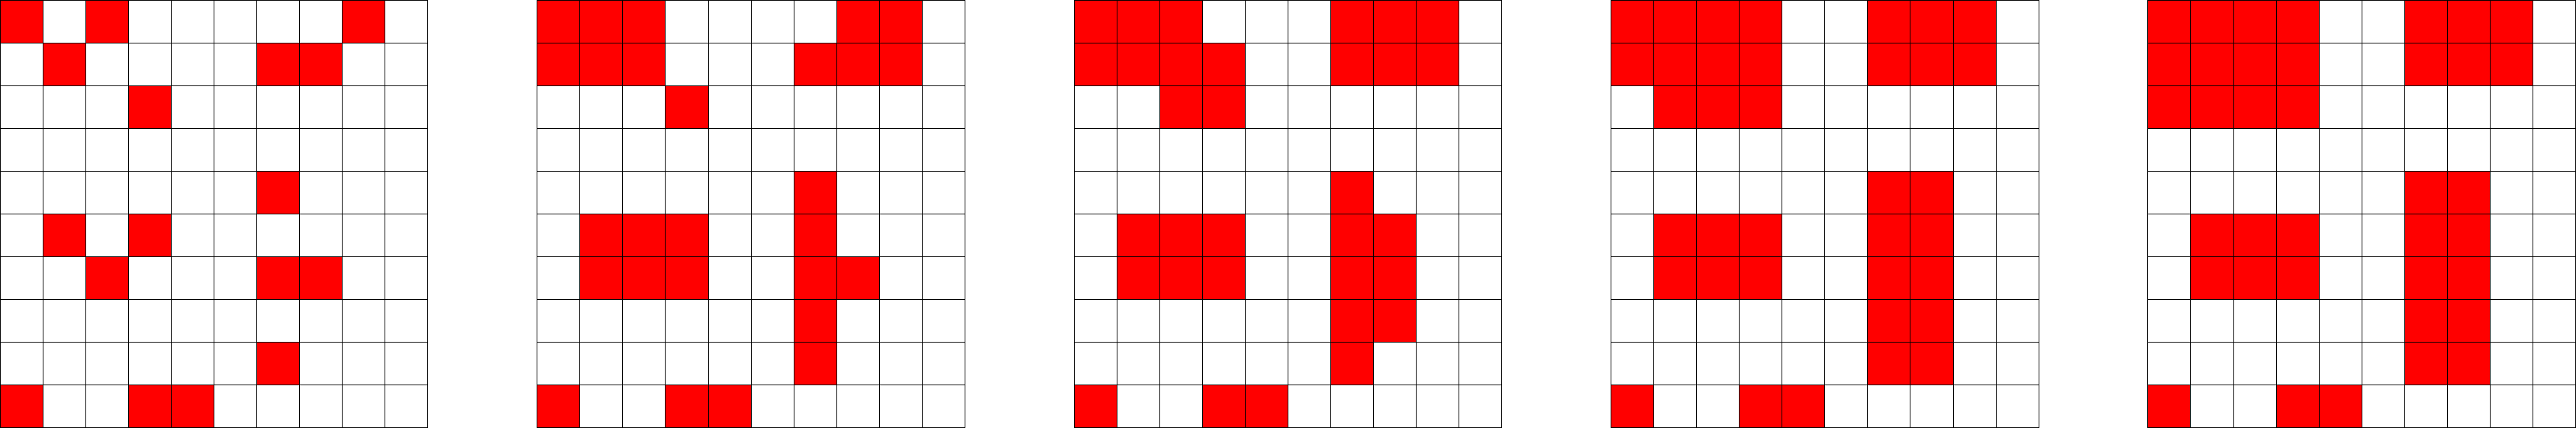
\includegraphics[width=\textwidth]{figures/1/simple_puzzle.pdf}
\caption{An arbitrary set of initially infected cells in the $10 \times 10$ lattice, and the stages of infection.}
\label{fig:simple_puzzle}
\end{figure} 

Before we present the solution,
%(which is particularly elegant and satisfying, and the reader is encouraged to play around with this problem on their own and get a feel for the behavior), 
let us take a moment to examine some properties of infectious sets and attempt to characterize what attributes might correspond to lethality. It should not take too long to observe that if an initial infection is in some way ``spread too thinly," then it will be unable to jump between infected areas, leading to gaps in infection, which we refer to as \emph{immune regions}. The perimeter of the lattice is particularly susceptible to this, as vertices there have fewer neighbors from whom they might be exposed. Heuristically, then, a lethal set must have the ability to effectively span the entire lattice, and must be particularly virulent along the perimeter. 

With this criteria in mind, we are able to make some educated guesses regarding the specific structure of sets that are likely to be lethal. In particular, we would like to consider the two starting infections illustrated in Figure \ref{fig:two_infections}. Notice that while Figure \ref{fig:two_infections} (\subref{fig:two_infections_b}) has far fewer perimeter infections, both (\subref{fig:two_infections_a}) and (\subref{fig:two_infections_b}) manage to form continuous bands of infected cells that appear to span the entire lattice after one step. Indeed, this fits with our notion of immune regions (or lack thereof), and we see that both infections will continue to propagate outwards from these bands until all cells become infected.

\begin{figure}[]
\centering
\begin{subfigure}{0.45\textwidth}
	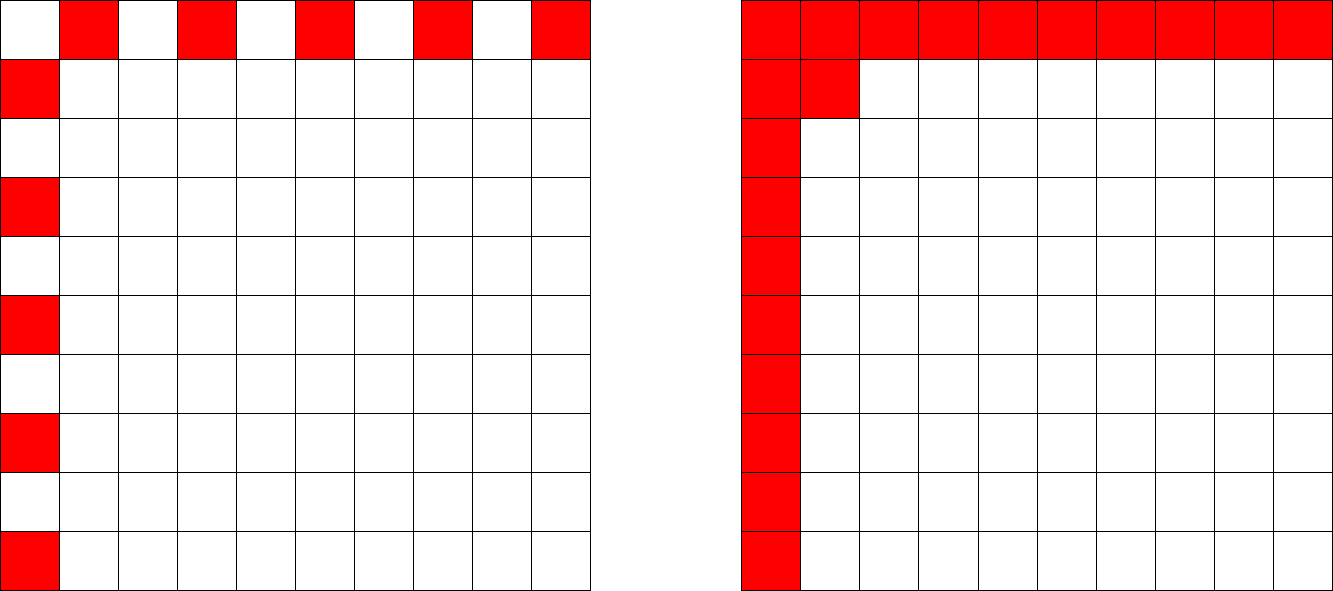
\includegraphics[width=\textwidth]{figures/1/two_infections_a.pdf}
	\caption{Perimeter construction.}
	\label{fig:two_infections_a}
\end{subfigure} \hfill%
\begin{subfigure}{0.45\textwidth}
	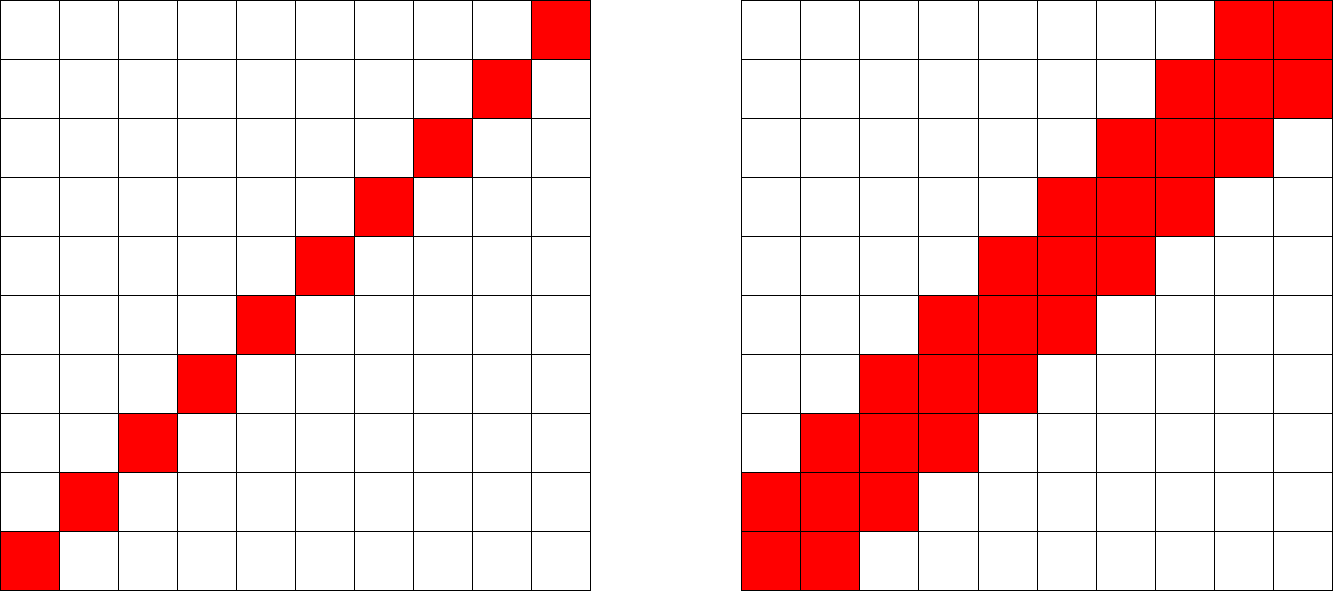
\includegraphics[width=\textwidth]{figures/1/two_infections_b.pdf}
	\caption{Diagonal construction.}
	\label{fig:two_infections_b}
\end{subfigure}
\caption{Two lethal sets and their resulting infections after one time-step.}
\label{fig:two_infections}
\end{figure} 

It is clear from Figure \ref{fig:two_infections} that we may obtain lethal sets on the $n \times n$ lattice of size $n$ by simply infecting the diagonal. What is less obvious is whether it is possible to improve upon this result. Perhaps the most natural first attempt at this is to remove an infection from one of the cells along the diagonal. However, this seems to form an immune region containing the removed cell. After some experimentation, one begins to believe it impossible to simultaneously satisfy the heuristic that a starting infection must span the lattice, while also using fewer than $n$ initial infections. The question therefore becomes: how do we prove it?

Consider the cumulative perimeter of infected regions. For a given infectious set $A$, let $P(A)$ be the total perimeter of the infected regions of $A$. Let $A_0$ be an initial infection, and observe that $P(A_0) \leq 4 |A_0|$. (This bound is only tight if no two infected cells are adjacent. Otherwise, the edge between such cells lies within the infected region, and cannot contribute to the infection's perimeter.) Observe that for any uninfected cell to become infected, it must abut at least two infected cells. Upon infection, the edges adjacent to these cells no longer lie on the infection's perimeter; additionally, the remaining edges of this newly infected cell contribute at most $2$ to this perimeter. All told, after infection, $P(A_1) \leq P(A_0)$. 

If we suppose that $A_0$ is a lethal set, then at some point in time, the entire grid will become infected. This infection will have a perimeter $4n$. Since this perimeter did not increase, $A_0$ must have originally had a perimeter of at least $4n$. Since each cell in $A_0$ can contribute at most $4$ to this perimeter, it must be the case that $|A_0| \geq n$. Our diagonal construction shows that $|A_0| \leq n$, and so we are able to conclude that $n$ is best possible.

This proof is an instance of the famous \emph{perimeter argument}, which has belonged to bootstrap percolation folklore since at least the work of Pete \cite{pete:1997}. In the following section, we present generalizations of this argument to higher dimensional rectangular grids.

\section{Bootstrap Percolation}

%Before presenting a proof, let us take a moment to formally define the process described above and develop some useful notation. 
The study of such cellular infection spread in grids (and, more generally, in graphs) is known in the literature as \emph{bootstrap percolation}, and was introduced in the 1970s by Chalupa et al. \cite{chalupa:1979} as a simplified model for the behavior of ferromagnetic fields. In their original 1979 paper, the authors research the stable structure of probabilistically selected initial infections. While this differs from the problem posed in Question \ref{que:simple_puzzle}, the rules for the spread of infection and its broad behavior remain the same. It is worth noting that a large portion of contemporary research on bootstrap problems is focused on questions of probabilistic nature; while these problems are certainly interesting and of merit, they do not fall within the scope of this thesis. Rather, we shall focus on those problems where we have specific control over the structure of the initial infections; in particular, we aim to determine the smallest lethal set on the Cartesian product of paths and cycles. 

Let us now define the problem in concrete terms. Let $G$ be a graph, let $r \geq 0$ and let $A_0 \subseteq V(G)$ be a set of initially infected vertices. Iteratively, infect those vertices of $G$ with at least $r$ infected neighbors. For all $t > 0$, let $A_t$ be the set of infected vertices at time step $t$. We then have
$$A_t = A_{t-1} \cup \{v \in V(G) : |N_G(v) \cap A_{t-1}| \geq r\},$$
where $N_G(v)$ is the set of vertices adjacent to $v$ in $G$. We define the \emph{closure} of $A_0$ under $r$-neighbor bootstrap percolation to be $[A_0] = \bigcup_{t=0}^{\infty} A_t$. We say that $A_0$ \emph{percolates} or is \emph{lethal} if $[A_0] = V(G)$. We define the smallest lethal set in a graph $G$ under $r$-neighbor bootstrap percolation by the quantity $m(G,r)$. We note that under these rules, it is not possible for vertices to become uninfected.

While it is possible to study bootstrap percolation on any graph $G$, much of the contemporary research focuses on multidimensional grids \cite{something}. We therefore introduce the following notation. For all $n \in \mathbb{N}$, let $[n] = \{1, 2, \dots, n\}$. Let the grid graph with vertex set $\prod_i^d [a_i]$ be denoted by $\prod_i^d [a_i]$. Note that $\prod_i^d [a_i] = P_{a_1} \square \cdots \square P_{a_d}$. Furthermore, define:
$$m(a_1, \dots, a_d, r) = m(\prod_i^d [a_i], r).$$

There are a number of natural generalizations of the problem posed in Question \ref{que:simple_puzzle}. In this thesis, we discuss those obtained by varying the structure of $G$ and the value of $r$. Below, we outline some of the existing results for graphs that are the Cartesian product of paths and cycles, and $r \in \{0, 1, 2, 3\}$. These results are summarized in Table \ref{tab:known_bounds}.

\begin{table}[]
\centering
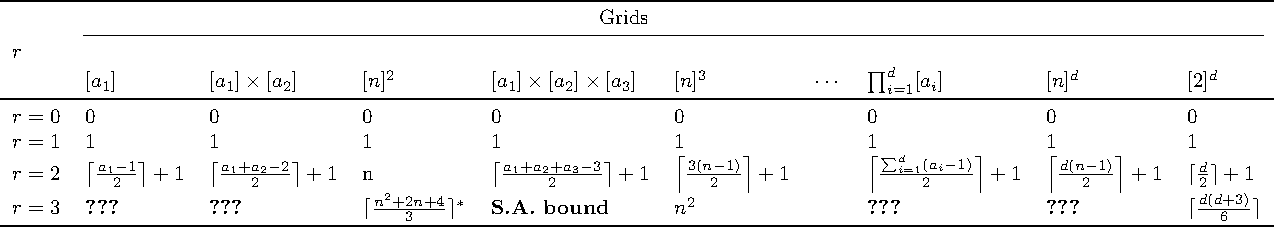
\includegraphics[width=\textwidth,origin=c]{tables/1/known_bounds.pdf}
\caption{A summary of known bootstrap percolation results for grids and the torus, $r \in \{0,1,2,3,d\}$.}
\label{tab:known_bounds}
\end{table} 

\subsection{Results on grids and tori}
\label{sec:result_summary}

In this section, we highlight major bootstrap percolation results on grids and tori. Some of the following bounds are not tight and require supplemental constructions, which are often difficult to obtain. We further sub-divide this discussion into results on the grid (of which there are many), and results on the torus (of which there are few).

\subsubsection{Grids}

From the puzzle posed in Question \ref{que:simple_puzzle}, we readily obtain variant problems by altering three parameters: the size and shape of the grid $G$, the grid's dimension $d$, and the threshold number of neighbors $r$. We examine each of these problems in turn.

In the prior discussion of the perimeter argument, we showed that for square grids $[n]^2$, $m([n]^2, 2) \geq n$, and verified this to be tight with a diagonal construction. The following result (attributed to Pete) generalizes this result to all rectangular grids $[a_1] \times [a_2]$. A proof is included for completeness. 

\begin{thm}
\label{thm:perimeter_rects}
For $a_1, a_2 \geq 1$,
$$m(a_1,a_2,2) = \ceil*{\frac{a_1+a_2-2}{2}}+1.$$
\end{thm}

\begin{proof}
We obtain a lower bound on $m(a_1,a_2,2)$ by applying the perimeter argument. Note that the perimeter of the $a_1 \times a_2$ grid is $2(a_1+a_2)$, and so the $m(a_1,a_2,2) \geq \ceil*{\frac{a_1+a_2}{2}}$. (We take the ceiling because the size of infected sets must be integral. See Figure \ref{fig:sa_construction_2d}.) For the upper bound, we proceed by induction on $a_1+a_2$. For $a_1+a_2 \leq 4$, the lethal sets in Figure \ref{fig:base_cases} match the lower bounds given by the perimeter argument (1, 2, 2, and 2, respectively). For $a_1+a_2 > 4$, suppose without loss of generality that $a_1 \leq a_2$, and so $a_2 \geq 3$. By hypothesis, $[a_1] \times [a_2-2]$ admits a lethal set $A_0$ at the perimeter bound. We show that $A_0$, plus the addition of any infection in the final column of $[a_1] \times [a_2]$, is lethal and matches the perimeter bound. 

Observe that $A_0$ infects all vertices of $[a_1] \times [a_2]$, apart from the final two columns. The additional vertex in the final column is then sufficient to infect all remaining healthy vertices. Finally, by incrementing $a_2$ by two, the perimeter bound is incremented by exactly one. This completes the proof.
\end{proof}

\begin{figure}[]
\centering
\begin{subfigure}{0.03\textwidth}
	
\includegraphics[width=\textwidth]{figures/1/1x1x1.pdf}
\end{subfigure} \hfill%
\begin{subfigure}{0.064\textwidth}
	
\includegraphics[width=\textwidth]{figures/1/1x2x1.pdf}
\end{subfigure} \hfill%
\begin{subfigure}{0.1\textwidth}
	
\includegraphics[width=\textwidth]{figures/1/1x3x1.pdf}
\end{subfigure} \hfill%
\begin{subfigure}{0.06\textwidth}
	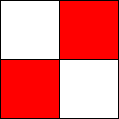
\includegraphics[width=\textwidth]{figures/1/2x2x1.pdf}
\end{subfigure}
\caption{Tight constructions for lethal sets where $a_1+a_2 \leq 4$.}
\label{fig:base_cases}
\end{figure} 

Let us take a moment to examine the issue of integrality in the perimeter bound. Non-integrality occurs either when adjacent vertices are infected in the same generation, or when a vertex is infected by more than $r$ neighbors. Note that in both cases, this decreases the perimeter of infection. One way to think about this is to consider each vertex as having ``infectious potential": vertices $v \in A_0$ can infect up to $d(v)$ healthy vertices, whereas vertices $v \in A_i$ for $i > 0$ can infect at most $d(v) - r$. An integral perimeter bound mandates that each vertex realize its potential, whereas a non-integral bound leaves a small margin for error. Figure \ref{fig:sa_construction_2d_a} illustrates the integral case, where each cell is infected by exactly two neighboring cells; this condition ensures that $P(A_i) = P([A_0])$ for all $i$. Conversely, in Figure \ref{fig:sa_construction_2d_b}, the cell demarcated with an ``X" experiences infection on three sides, thereby reducing its infectious potential. The existence of such a cell is guaranteed by the fact the perimeter bound in this case is non-integral. 

\begin{figure}[]
\centering
\begin{subfigure}{0.4\textwidth}
	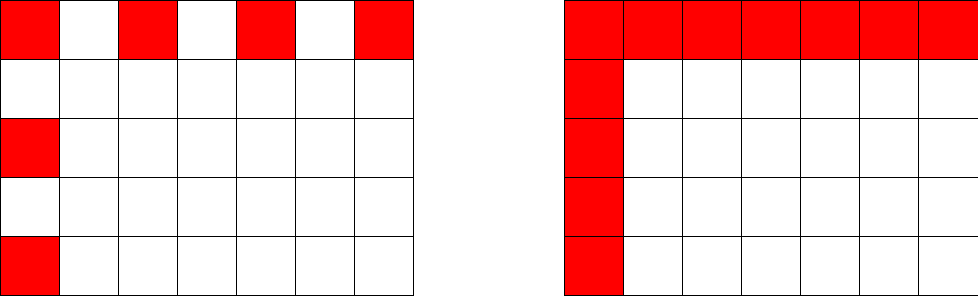
\includegraphics[width=\textwidth]{figures/1/5x7x1.pdf}
	\caption{$a+b \equiv 0 \pmod 2$}
	\label{fig:sa_construction_2d_a}
\end{subfigure} \hfill%
\begin{subfigure}{0.45\textwidth}
	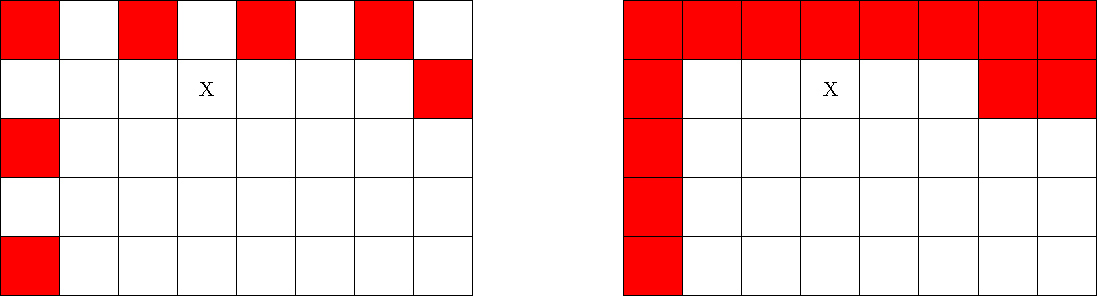
\includegraphics[width=\textwidth]{figures/1/5x8x1.pdf}
	\caption{$a+b \equiv 1 \pmod 2$}
	\label{fig:sa_construction_2d_b}
\end{subfigure}
\caption{Tight constructions for lethal sets on the $[a] \times [b]$ grid.}
\label{fig:sa_construction_2d}
\end{figure} 

We can further generalize for the case of $r=2$. In 2006, Balogh and Bollobas \cite{balogh:2006} proved the following general form of Theorem \ref{thm:perimeter_rects} for all $d$-dimensional hypercubes $(a_1, \dots, a_d)$, $a_i \geq 1$:

\begin{thm}[Balogh]
\label{thm:complete_r_2}
For $d \geq 1$ and $a_1, \dots, a_d \geq 1$, 
$$m(a_1, \dots, a_d, 2) = \ceil*{\frac{\sum_{i=1}^d (a_i-1)}{2}}+1.$$
\end{thm}

Theorem \ref{thm:complete_r_2} completes the picture for infections with a threshold of two on grids. The next question is whether similar results exist for larger $r$. Unfortunately, while generalizing to $d$-dimensional grids yields nice results for $r=2$, attempts to obtain a holistic understanding of $m(a_1, \dots, a_d, r)$ for arbitrary $r$ have been largely fruitless. Even the case of $r=3$ remains stubbornly inaccessible for nearly all large $d$. However, certain breakthroughs have been made in the following circumstances: $d=2$, $d=3$, and $G=[2]^d$.

We first consider 3-neighbor percolation on two-dimensional square grids. In 2021, Benevides et al. proved that 
$$m(n,n,3) = \ceil*{\frac{n^2+2n+4}{3}}$$
for even $n$, and 
$$\ceil*{\frac{n^2+2n}{3}} \leq m(n,n,3) \leq \ceil*{\frac{n^2+2n}{3}} + 1$$
for odd $n$. Additionally, they showed that these bounds are tight for odd $n$: if $n = 5 \pmod 6$, or $n = 2^k - 1$ for some $k \in \mathbb{N}$, then $m(n,n,3) = \ceil{\frac{n^2+2n}{3}}$; and if $n \in \{9,13\}$, then $m(n,n,3) = \ceil{\frac{n^2+2n}{3}} + 1$. Constructions that achieve this bound are illustrated in Chapter 7. We add to this picture with the following theorem, proven in Chapter 6, and corollary:

\begin{thm}
\label{thm:2d_rectangle}
Suppose that $a, b \geq 1$ such that
$$m(a,b,3) = \frac{2ab+a+b}{3}.$$
Then there exists $k \geq 1$ such that $a=b=2^k-1$.
\end{thm}

\begin{cor}
For all $n \geq 1$,
$$ m(n,n,3) =
\begin{cases} 
      \ceil*{\frac{n^2+2n+4}{3}} & n \equiv 0 \pmod 2 \\
      \frac{n^2+2n}{3} & n = 2^k-1, \; k \in \mathbb{N} \\
      \frac{n^2+2n+1}{3} & n \equiv 5 \pmod 6 \\
      \frac{n^2+2n+3}{3} & \text{otherwise.}
   \end{cases}
$$
\end{cor}

\begin{proof}
The first three cases follow from Theorem 1 of \cite{benevides:2021} and the observation that if $n \equiv 5 \pmod 6$, then $\ceil{\frac{n^2+2n}{3}} = \frac{n^2+2n+1}{3}$. In the final case, $n$ is congruent to either 1 or 3 modulo 6. This implies that $n^2 + 2n$ is divisible by three. From Theorem 1 of \cite{benevides:2021}, we have that $m(n,n,3) \leq \frac{n^2+2n+3}{3}$. Furthermore, since $n$ is not of the form $2^k-1$, it follows from Theorem \ref{thm:2d_rectangle} that $m(n,n,3) > \frac{n^2+2n}{3}$. Therefore, $m(n,n,3) = \frac{n^2+2n+3}{3}$.
\end{proof}

This result resolves the question of the minimum lethal set for two dimensional square grids. For the more general case of rectangular grids, the problem remains unsolved. However, we are able to achieve an upper bound of $m(a,b,3) \leq \ceil{\frac{ab+a+b+6}{3}}$ and a lower bound (described below) of $m(a,b,3) \geq \ceil{\frac{ab+a+b}{3}}$, for all $a,b > 1$. Further discussion of these results can be found in Chapter 6.

One significant and well-known result for 3-neighbor percolation on two- and three-dimensional grids is the following lower bound, taken as a three-dimensional analogue of the perimeter bound. This result is referenced frequently throughout this document, and referred to interchangeably as the \emph{surface area} or \emph{SA bound}. We prove the statement in full generality, while noting that we only make use of the case where $d=3$. We also note that, like the perimeter bound, the following proof belongs to bootstrap percolation folklore, and appears to have been first published in 1997 by Balogh and Pete \cite{balogh_and_pete}.

\begin{thm}
\label{thm:sa_bound}
For any $d \geq 1$ and $a_1, a_2, \dots, a_d \geq 1$, 
$$m(a_1,a_2, \dots, a_d,d) \geq \frac{\sum_{j=1}^d \prod_{i \neq j} a_i}{d}.$$
\end{thm}

\begin{proof}
We apply the same invariant strategy presented in the perimeter argument. For simplicity, consider $\prod_{i=1}^d[a_i]$ to be embedded within the larger graph $\prod_{i=1}^d \{0, \dots, a_i + 1\}$. Note that in $\prod_{i=1}^d \{0, \dots, a_i + 1\}$, each vertex $v \in \prod_{i=1}^d[a_i]$ has degree $2d$. Let $A_0$ be a lethal set in $\prod_{i=1}^d[a_i]$ under the $d$-neighbor bootstrap process. Let $A_t$ be the set of infected vertices in $\prod_{i=1}^d[a_i]$ at generation $t$. Denote by $m_t$ the number of edges between vertices $u \in A_t$ and $v \in \prod_{i=1}^d[a_i] \setminus A_t$. %We show that the sequence $m_0, m_1, m_2, \dots$ is monotonically decreasing. 
We show that $m_{t-1} \geq m_t$ for all $t> 0$. 

%Let $N = |A_t - A_{t-1}|$, and let $v_1, \dots, v_N$ be an arbitrary ordering on the vertices of $A_t \setminus A_{t-1}$. 
By definition, each vertex $v \in A_t \setminus A_{t-1}$ has at least $d$ neighbors in $A_{t-1}$. Therefore, since $d(v) = 2d$, $v$ has no more than $d$ neighbors outside of $A_t$. This implies that the number of edges from $A_{t-1} \cup \{v\}$ to $\prod_{i=1}^d[a_i] \setminus A_{t-1} \cup \{v\}$ cannot exceed $m_{t-1}$. Furthermore, this holds for every vertex $v \in A_{t-1}$, and so $m_{t-1} \geq m_t$. 

Since $A_0$ is lethal, we have that 
$$2d|A_0| \geq m_0 \geq m_1 \geq \dots \geq 2 \sum_{j=1}^d \prod_{i \neq j} a_i,$$ 
where the final expression gives the total number of edges between the fully infected grid and the surrounding larger grid. Dividing through by $2d$ gives the result.
\end{proof}

We note that the prior argument is precisely the same as the so-called perimeter argument outlined on Page 2. Here, the quantity $m_t$ is a $d$-dimensional analogue of the perimeter of infection $P(A_t)$ at time-step $t$, and the lower bound
$$2\sum_{j=1}^d \prod_{i \neq j} a_i$$
is the $d$-dimensional ``perimeter" of the grid. Again, observe that equality can only be obtained when no vertices of $A_0$ are adjacent, and all vertices $v \in A_{t>0}$ are infected by exactly $d$ neighbors. Any imprecision causes a reduction in ``perimeter" of two units, corresponding to a $1/d$ increase in the bound. 

The primary aim of this thesis is to prove that the surface area bound is tight for sufficiently large grids when $r=3$. This process employs a number of general constructions (discussed in Chapter 7), as well as a recursive strategy (Chapter 3). In Chapter 5, we prove the following result:

\begin{thm}
\label{thm:main_result}
For all $a_1, a_2, a_3 \geq 11$, 
$$m(a_1,a_2,a_3,3) = \ceil*{\frac{a_1a_2+a_2a_3+a_1a_3}{3}}.$$
\end{thm}

Unfortunately, the complete resolution of the $r=3$ case on grids remains elusive. Tight constructions exist for cubes $[n]^3$ and hypercubes $[2]^d$, but in general bounds are difficult to obtain. Worse, for $r>3$, the only additional result beyond the surface area bound addresses the very specific case of $r$-dimensional cubes. Open problems abound.

\subsubsection{Tori}

In addition to varying the parameters $r$ and $d$, we might also change the very structure of $G$. It is natural to shift from grids (the Cartesian product of paths) to tori (the Cartesian product of cycles). In fact, it could be argued that bootstrap percolation on the torus is \emph{more} natural than the grid, since tori are regular and grids are not. This problem has been studied by Benevides et al. In 2021, they obtained the following lower bound for the Cartesian product of two cycles \cite{benevides:2021}. Their proof is included here for completeness.

\begin{thm}
\label{thm:torus_lb}
For $a, b \geq 1$,
$$m(C_a \square C_b,3) \geq \ceil*{\frac{ab +1}{3}}.$$
\end{thm}

\begin{proof}
Let $G = C_a \square C_b$, and let $I$ be a lethal set on $G$. Let $H = V(G) \setminus I$, and note that $|H| = ab - |I|$. Let $m_{H}$ be the number of edges in the subgraph of $G$ induced by $H$, and $m_{IH}$ be the number of edges between vertices in $I$ and vertices in $H$. Note that $m_{IH}$ is similar to the notion of perimeter on a grid.

Observe that $G[H]$ must be cycle-free: cycles in $G[H]$ constitute immune regions, and contradict the lethality of $I$. Therefore, $G[H]$ is a forest, and so $m_H = |H| - c$, where $c$ is the number of components in $G[H]$. Additionally, note that $m_{IH} \leq 4|I|$, since $G$ is $4$-regular. Finally, observe that the total degree of $G[H]$ is $2m_H = 4|H| - m_{IH}$.

Chaining together these inequalities, we obtain:
\begin{align*}
4|I| \geq m_{IH} &= 4|H| - 2m_H \\
&= 4|H| - 2(|H| -c) = 2|H| + 2c \\
&= 2(ab-|I|) + 2c
\end{align*}
Combining like terms and simplifying, we have
$$|I| \geq \frac{ab +c}{3} \geq \frac{ab +1}{3}.$$
\end{proof}

Observe that the conditions $c \geq 1$ and $m_{IH} \leq 4|I|$ prevent us from obtaining strict equality. Specifically, if $I$ is lethal, $G[H]$ has one component, and no vertices in $I$ are adjacent, then $|I|$ is minimized. Note that these conditions are quite similar to those on grids; the specific difference is that equality in the bound on grids mandates that no vertex be infected by more than $r$ neighbors, whereas equality on three-dimensional tori requires this inefficiency be centered on one particular vertex. 

% other semi-related problems in bootstrap percolation
\section{Other Problems}

In this section, we provide a cursory overview of some other related areas of study in bootstrap percolation. We highlight problems regarding the number of iterations necessary to infect all vertices on a graph.

\section{Structure of this Thesis}

As stated by Theorem \ref{thm:main_result}, the primary goal of this thesis is to prove a tight bound for 3-neighbor bootstrap percolation on three-dimensional grids of sufficiently large size. This task requires the use of two major lemmas, as well as both original and previously published ideas and constructions. In an effort to present this material in a coherent manner, the paper is structured as follows. 

Chapters 2 and 3 are dedicated to building a conceptual and intuitive framework upon which to prove Theorem \ref{thm:main_result}. In Chapter 2, we categorize and present percolating sets on both divisible and non-divisible grids, and discuss the differences between these cases. In Chapter 3, we prove two lemmas allowing us to develop large families of lethal sets that match the surface area bound. 

Chapters 4 and 5 leverage the results of Chapter 3 to prove Theorem \ref{thm:main_result}. In Chapter 4, we show that all divisible grids $(a_1,a_2,a_3)$, $a_1 \leq a_2 \leq a_3$ admit lethal sets matching the SA bound, and in Chapter 5, we extend this result to all grids of size 11. Chapter 6 further builds on this, highlighting some new results for 3-neighbor percolation on grids of the form $(a_1,a_2,1)$.

Chapter 7 proves the constructions presented in Chapter 2.

Finally, Chapters 8, 9 and 10 wrap up the discussion with a summary of the programmatic techniques used to discover lethal sets, helpful software resources for future research, how the results of this thesis may be helpful in pursuit of results on the torus, and recommendations for future research in similar and related problems. 

% proof of perimeter bound and generalization to surface area bound
% "So we have a goal, and now the question becomes whether or not it is possible to obtain this goal in all cases through constructions."

% "We shall see that generally (and especially for large grids), it is possible to find constructions that percolate at the lower bound. However, some smaller cases seem to contain unavoidable regions of immunity."
% For this reason, it will be helpful to expand on our observations about immune regions and perimeter infections."
% discussion about the notion of immune regions

% Possible discussion of existing results, where our results fit into the literature and presentation of the table??

% Lay out the structure of this paper. 
% "We show that through a clever recursive construction we are able to obtain percolating sets at the lower bound for all grids of size at least 11, and at least 5 for divisibility cases."
% "We establish a set of cases for which the lower bound cannot be met, and present a best upper bound for these cases."
% 1. Introduction
% 2. Recursion
% 3. Divisibility cases
% 4. All cases
% 5. Thickness 1
% 6. Constructions
% 7. Visualization tool??
% 8. The torus?

% vvv ONE GIANT COMMENT vvv
% COMMENT
% COMMENT
% COMMENT
% COMMENT
% COMMENT
% COMMENT
% COMMENT
% COMMENT
\begin{comment}
In the following chapter, we lay out in formal terms those lemmas necessary to understand and prove Theorem \ref{thm:main_result}. In particular, we discuss the recursive technique that permits the construction of lethal sets on grids of arbitrary large size, as well as a number of characteristics of lethal sets. We distinguish between two types of grids--those with integral \emph{SA bound}, and those without--and show that it is possible obtain tight constructions on non-integral grids from integral grids. 

In Chapter 3, we prove that there exist lethal sets at the S.A. bound for all integral grids of size at least 5. This chapter makes significant use of a number of existing constructions, described in Chapter 6, as well as the recursive strategy introduced in Chapter 2. 

Chapter 4 extends the results of Chapter 3 to all grids of size at least 11 with non-integral surface area bound. 

Chapter 5 considers the specific case of grids of the form $(a,b,1)$, and answers a question posed in Benevides et al. \cite{benevides:2022} regarding the existence of tight lethal sets on non-square grids. 

Chapter 6 is dedicated to presenting and proving the lethality of sets on a number of grids, and families of grids. 

Chapter 7 discusses some of the programmatic techniques used to evaluate, examine and explore the behavior of percolating sets. 

Chapter 8 examines the problem of bootstrap percolation on the 3- and 4-torus, and presents a class of constructions within constant size of the lower bound. 

Chapter 9 presents open questions related to the results presented in this thesis, and provides some suggestions for future research.

% COMMENT

% r=0 and r=1
\subsection{$m(G,0)$ and $m(G,1)$} 

In the case where $r \in \{0,1\}$, the specific structure of $G$ is unimportant. We have the following results:

\begin{thm}
For all undirected, simple graphs $G$, $m(G,0) = 0$.
\end{thm}

\begin{proof}
As cells need not be adjacent to infections to become infected, $A_1 = V(G)$, and so $A_0 = \emptyset$ is lethal.
\end{proof}

\begin{thm}
Let $G$ be an undirected, simple graph with $c$ components. Then $m(G, 1) = c$.
\end{thm}

\begin{proof}
Let $A_0$ be lethal. As infections spread along all edges, it is both necessary and sufficient for each connected component of $G$ to contain exactly one vertex of $A_0$. Therefore, $|A_0| = m(G,1) = c$.
\end{proof}

% r=2
\subsection{$m(G,2)$} 

We consider three classes of generalizations: the Cartesian product of paths, the Cartesian product of cycles, and the Cartesian product of both. 

\subsubsection{Grid: $P_a \square P_b$}

Recall from the discussion of Question \ref{que:simple_puzzle} that $m(n, n,2) = n$, where the tight construction for the lower bound is given by a diagonal infection expanding laterally outwards. We generalize this result to all rectangular grids.

\begin{thm}
For $a, b \geq 1$,
$$m(a,b,2) = \ceil*{\frac{a+b-2}{2}}+1.$$
\end{thm}

\begin{proof}
We obtain a lower bound on $m(a,b,2)$ by applying the perimeter argument. Note that the perimeter of the $a \times b$ grid is $2(a+b)$, and so the $m(a,b,2) \geq \ceil*{\frac{a+b}{2}} = \ceil*{\frac{a+b-2}{2}}+1$. (We take the ceiling because the size of infected sets must be integral.) For the upper bound, we generalize the construction illustrated in Figure \ref{fig:two_infections_a} to rectangular grids. Consider two cases: $a+b \equiv 0 \pmod 2$ and $a+b \equiv 1 \pmod 2$ (see Figure \ref{fig:sa_construction_2d}). Note that in both cases, the initial infectious set $A_0$ is lethal. Furthermore, note that in Figure \ref{fig:sa_construction_2d_a}, $|A_0| = \frac{a+b}{2}$, and in Figure \ref{fig:sa_construction_2d_b}, $|A_0| = \ceil*{\frac{a+b}{2}}$. In both cases, this agrees with the perimeter bound.
\end{proof}

It is worth noting that the integrality condition on the perimeter bound corresponds exactly to the non-existence of cells that are infected by more than two neighbors. In Figure \ref{fig:sa_construction_2d_a}, each cell is infected by exactly two neighboring cells; this condition ensures that $P(A_i) = P([A_0])$ for all $i$. Conversely, in Figure \ref{fig:sa_construction_2d_b}, the cell demarcated with an ``X" experiences infection on three sides. The existence of such a cell is guaranteed by the fact the perimeter bound in this case is non-integral. 

\begin{figure}[]
\centering
\begin{subfigure}{0.4\textwidth}
	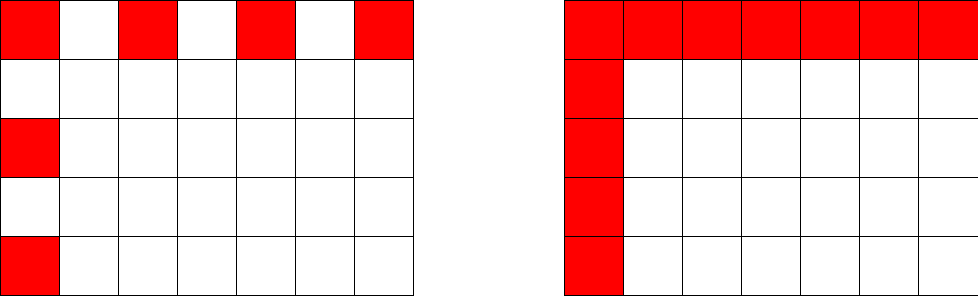
\includegraphics[width=\textwidth]{figures/1/5x7x1.pdf}
	\caption{$a+b \equiv 0 \pmod 2$}
	\label{fig:sa_construction_2d_a}
\end{subfigure} \hfill%
\begin{subfigure}{0.45\textwidth}
	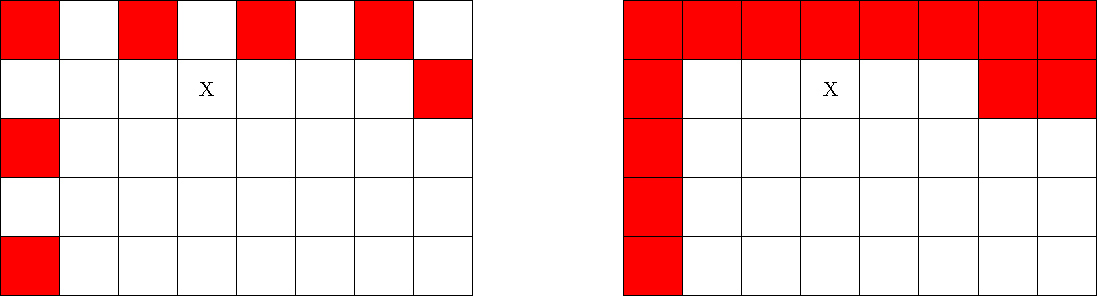
\includegraphics[width=\textwidth]{figures/1/5x8x1.pdf}
	\caption{$a+b \equiv 1 \pmod 2$}
	\label{fig:sa_construction_2d_b}
\end{subfigure}
\caption{Tight constructions for lethal sets on the $[a] \times [b]$ grid.}
\label{fig:sa_construction_2d}
\end{figure} 

\subsubsection{Grid: $P_a \square P_b \square \dots \square P_d$}

In a paper by Balogh and Bollobas \cite{balogh:2006}, the above result is generalized to all $d$-dimensional hypercubes $(a_1, \dots, a_d)$, $a_i \geq 1$. 

\begin{thm}
For $d \geq 1$ and $a_1, \dots, a_d \geq 1$, 
$$m(a_1, \dots, a_d, 2) = \ceil*{\frac{\sum_{i=1}^d (a_i-1)}{2}}+1.$$
\end{thm}

% r=3
\subsection{$m(G,3)$} 

We discuss a further generalization of the perimeter argument to higher dimensions. We show that this argument allows us to obtain nice bounds on 3-neighbor percolation in two and three-dimensional grids. We give a lower bound on the size of lethal sets in the 3-torus and 4-torus. We highlight the main theorem of this thesis.

\subsubsection{Grid: $P_n \square P_n$}

In 2021, Benevides et al. proved that 
$$m(n,n,3) = \ceil*{\frac{n^2+2n+4}{3}}$$
for even $n$, and 
$$\ceil*{\frac{n^2+2n}{3}} \leq m(n,n,3) \leq \ceil*{\frac{n^2+2n}{3}} + 1$$
for odd $n$. Additionally, they showed that these bounds are tight for odd $n$: if $n = 5 \pmod 6$, or $n = 2^k - 1$ for some $k \in \mathbb{N}$, then $m(n,n,3) = \ceil{\frac{n^2+2n}{3}}$; and if $n \in \{9,13\}$, then $m(n,n,3) = \ceil{\frac{n^2+2n}{3}} + 1$. Constructions that achieve this bound are illustrated in Chapter 5. We add to this picture with the following theorem, proven in Chapter X, and corollary:

\begin{thm}
\label{thm:2d_rectangle}
Suppose that $a, b \geq 1$ such that
$$m(a,b,3) = \frac{2ab+a+b}{3}.$$
Then there exists $k \geq 1$ such that $a=b=2^k-1$.
\end{thm}

\begin{cor}
For all $n \geq 1$,
$$ m(n,n,3) =
\begin{cases} 
      \ceil*{\frac{n^2+2n+4}{3}} & n \equiv 0 \pmod 2 \\
      \frac{n^2+2n}{3} & n = 2^k-1, \; k \in \mathbb{N} \\
      \frac{n^2+2n+1}{3} & n \equiv 5 \pmod 6 \\
      \frac{n^2+2n+3}{3} & \text{otherwise.}
   \end{cases}
$$
\end{cor}

\begin{proof}
The first three cases follow from Theorem 1 of \cite{benevides:2021} and the observation that if $n \equiv 5 \pmod 6$, then $\ceil{\frac{n^2+2n}{3}} = \frac{n^2+2n+1}{3}$. In the final case, $n$ is congruent to either 1 or 3 modulo 6. This implies that $n^2 + 2n$ is divisible by three. From Theorem 1 of \cite{benevides:2021}, we have that $m(n,n,3) \leq \frac{n^2+2n+3}{3}$. Furthermore, since $n$ is not of the form $2^k-1$, it follows from Theorem \ref{thm:2d_rectangle} that $m(n,n,3) > \frac{n^2+2n}{3}$. Therefore, $m(n,n,3) = \frac{n^2+2n+3}{3}$.
\end{proof}

This result resolves the question of the minimum lethal set for two dimensional square grids. For the more general case of rectangular grids, the problem remains unsolved. However, we are able to achieve an upper bound of $m(a,b,3) \leq \ceil{\frac{ab+a+b+6}{3}}$ for all $a,b > 1$. Further discussion of these results can be found in Chapter X.

\subsubsection{Grid: $P_a \square P_b \square P_c$}

%Observe that the surface area bound presented above applies directly to 3-dimensional grids. State the main theorem of this thesis. 
Surprisingly, it is possible to extend the perimeter argument to higher dimensions \cite{przykucki:2019}. This provides a lower bound on $m(a_1,a_2,a_3,3)$ of $\ceil{\frac{a_1a_2+a_2a_3+a_1a_3}{3}}$. We refer to this quantity as the \emph{surface area bound}. In Chapters 2 and 3, we use a recursive strategy to prove that the surface area bound is met for all sufficiently large grids. 

\begin{thm}
\label{thm:main_result}
For all $a_1, a_2, a_3 \geq 11$, 
$$m(a_1,a_2,a_3,3) = \ceil*{\frac{a_1a_2+a_2a_3+a_1a_3}{3}}.$$
\end{thm}

\subsubsection{Grid: $P_a \square P_b \square \dots \square P_d$}

Do we have a bound here?

\subsubsection{Torus: $C_a \square C_b$}

A lower bound for the Cartesian product of two cycles is given in Benevides \cite{benevides:2021}. Their proof is included here for completeness.

\begin{thm}
\label{thm:torus_lb}
For $a, b \geq 1$,
$$m(C_a \square C_b,3) \geq \ceil*{\frac{ab +1}{3}}.$$
\end{thm}

\begin{proof}
Let $G = C_a \square C_b$, and let $I$ be a lethal set on $G$. Let $H = V(G) \setminus I$, and note that $|H| = ab - |I|$. Let $m_{H}$ be the number of edges in the subgraph of $G$ induced by $H$, and $m_{IH}$ be the number of edges between vertices in $I$ and vertices in $H$. Note that $m_{IH}$ is similar to the notion of perimeter on a grid.

Observe that $G[H]$ must be cycle-free: cycles in $G[H]$ constitute immune regions, and contradict the lethality of $I$. Therefore, $G[H]$ is a forest, and so $m_H = |H| - c$, where $c$ is the number of components in $G[H]$. Additionally, note that $m_{IH} \leq 4|I|$, since $G$ is $4$-regular. Finally, observe that the total degree of $G[H]$ is $2m_H = 4|H| - m_{IH}$.

Chaining together these inequalities, we obtain:
\begin{align*}
4|I| \geq m_{IH} &= 4|H| - 2m_H \\
&= 4|H| - 2(|H| -c) = 2|H| + 2c \\
&= 2(ab-|I|) + 2c
\end{align*}
Combining like terms and simplifying, we have
$$|I| \geq \frac{ab +c}{3} \geq \frac{ab +1}{3}.$$
\end{proof}

Observe that the conditions $c \geq 1$ and $m_{IH} \leq 4|I|$ prevent us from obtaining strict equality. Specifically, if $I$ is lethal, $G[H]$ has one component, and no vertices in $I$ are adjacent, then $|I|$ is minimized. 

\subsubsection{Torus: $C_a \square C_b \square C_c$}

Present the lower bound and note that we are able to obtain constructions within constant distance of this bound for arbitrarily large grids.

%In the context of question \ref{que:simple_puzzle}, $G = P_{10} \Osq P_{10}$, and our diagonal construction shows us that $m(2,G) \leq 10$. In general, we have observed that for $G = P_n \Osq P_n$, $m(2, G) \leq n$. Now, let us prove that the bound is, in fact, tight. 

\begin{prop}
\label{prop:tight_perimeter}
For all $n \geq 1$, 
$$m([n]^2, 2) = n.$$
\end{prop}

\begin{proof}
The upper bound follows from our diagonal construction in figure \ref{fig:two_infections} (\subref{fig:two_infections_b}). The lower bound is given by the famous ``perimeter argument". Consider the $n\times n$ grid $G$, given by $G = P_n \Osq P_n$. Let $A_0 \subseteq V(G)$ be a set of initially infected cells. We claim that the total perimeter of all infected regions in $G$ is monotonically decreasing as a function of the time-step $t$. Consider an arbitrary healthy cell $c$. In order for $c$ to become infected, at least two of its edges must abut infected cells. However, this implies that (upon infection of $c$) these edges are absorbed within the newly expanded infected region, thereby reducing the perimeter of infection by two. As $c$ contains at most two un-absorbed edges, the perimeter of infection cannot increase. 

Since a lethal set will infect the entire grid, and therefore have a final perimeter of infection of $4n$, it follows that the perimeter of infection of $A_0$ must be at least $4n$, and so $m([n]^2, 2) \geq n.$
\end{proof}

This proof appears in \cite{przykucki:2019}, although it has been an established result in bootstrap percolation ``folklore" for considerably longer. We should like to make a few additional observations. 

First, note that we have used the following three expressions to describe the same graph $G$:

\begin{center}
\begin{enumerate*}[label=\roman*),itemjoin={\qquad}]
\item $n \times n$
\item $P_n \Osq P_n$
\item $[n]^2.$
\end{enumerate*}
\end{center}
\vspace{0.2in}

\noindent The notation in (i) is useful when discussing the shape of low dimensional, asymmetric grids. We use the notation in (ii) to remind readers that the fundamental structure in bootstrap percolation problems is a graph, and to suggest possible extensions of the problem discussed in this thesis to other similar objects. The notation in (iii) is the standard way to describe the vertex set of a grid graph, and can readily be generalized to any dimension $d$ by writing $[n]^d$. In a slight abuse of notation, we use $[n]^d$ to represent the entire graph $G$, and draw edges between vertices that differ by exactly one in exactly one coordinate. 

Second, the fact that we have used the notation $[n]^2$ in Proposition \ref{prop:tight_perimeter} suggests that we can generalize to higher dimensional grids $[n]^d$. Indeed, simply observe that for a given hypercube cell to become infected, it must donate at least $d$ of its $2d$ hyperplane faces to the infected region, thereby at most maintaining the current $(d-1)$-perimeter of infection. The following theorem summarizes this result.  

\begin{thm}
\label{thm:square_sa_bound}
For all $n,d \geq 1$, 
$$m([n]^d, d) \geq n^{d-1}.$$
\end{thm}

More generally, denote by $(a_1, \dots, a_n)$ the grid graph with vertex set $V = \{(i_1,\dots,i_n) \mid i_1 \in [a_1], \dots, i_n \in [a_n]\}$, and edge set $E = \{uv \mid u,v \text{ differ by one in exactly one coordinate}\}$. The following theorem provides a general lower bound on the size of lethal sets for all such graphs. 

\begin{thm}
\label{thm:general_sa_bound}
Let $G = (a_1, \dots, a_d)$, for $a_1, \dots, a_d, d \geq 1$. Then:
$$m(G, d) \geq \text{ sum of products of all subsets of size d-1, divided by d}.$$
\end{thm}

\begin{proof}
The proof follows the same high-dimensional surface area argument outlined above. 
\end{proof}

We highlight the three-dimensional instance of Theorem \ref{thm:general_sa_bound} in Corollary \ref{cor:sa_bound}, as it will prove particularly useful in the following chapters. We refer to this bound as the \emph{surface area} or \emph{S.A. bound}.

\begin{cor}
\label{cor:sa_bound}
Let $G = (a, b, c)$, for $a, b, c \geq 1$. Then:
$$m(G, 3) \geq \ceil*{\frac{ab + bc + ca}{3}}.$$
\end{cor}

\begin{proof}
Follows directly from Theorem \ref{thm:general_sa_bound}.
\end{proof}

While it has been shown that tight constructions exist for grids of the form $[n]^d$, where $r=d$, the problem of determining the existence of similar constructions for rectangular grids remains unsolved. In this thesis, we focus our attention on the particular case of $d=3$ and show that $m(a,b,c, 3) = \ceil*{\frac{ab + bc + ca}{3}}$ for all $a,b,c \geq 11$. 

% Separation of two commented out sections
% COMMENT
% COMMENT
% COMMENT
% COMMENT
% COMMENT

The problem of bootstrap percolation was first introduced in the 1970s by Chalupa et al. \cite{chalupa:1979} as a simplified model for the behavior of ferromagnetic fields. In their original paper, the authors describe bootstrap percolation as the stabilization of a probabilistically occupied lattice, where each occupied site must be adjacent to at least $m$ occupied neighbors. A re-rendering of the examples given in the original 1979 paper is presented in figures 1 and 2. 

In this original problem, the authors are interested in the structural patterns of these stable arrangements. Put differently, given a set of randomly distributed occupants on a $d$-dimensional lattice, what configuration can we expect these occupied sites to fall into, subject to the constraint that each occupied site is adjacent to at least $m$ other occupants? In this construction, a probabilistically populated lattice is iteratively de-populated until it reaches a stable state. 

Alternatively, we might consider the behavior of a population as it grows, instead of shrinks. In this model, it is useful to consider the population as harboring an infection that steadily spreads from site to site, subject to population density. We shall consider these infections to take place on a graph, with vertices representing members of our population (sites), and edges indicating adjacency. In formal terms: let $G$ be a graph and $A_0 \subseteq V(G)$ be a set of initially infected vertices. Iteratively, at every time step, infect those vertices of $G$ with at least $r$ infected neighbors. For all $t > 0$, let $A_t$ be the set of infected vertices at time step $t$. We then have
$$A_t = A_{t-1} \cup \{v \in V(G) : |N_G(v) \cap A_{t-1} \geq r\},$$
where $N_G(v)$ is the set of vertices adjacent to $v$ in $G$. We define the \emph{closure} of $A_0$ under $r$-neighbor bootstrap percolation to be $[A_0] = \bigcup_{t=0}^{\infty} A_t$. This is analogous to the stable states introduced in \cite{chalupa:1979}. We say that $A_0$ \emph{percolates} or is \emph{lethal} if $[A_0] = V(G)$. We note that under these rules, it is not possible for vertices to become uninfected. 

Perhaps the most natural extremal question regarding $r$-neighbor bootstrap percolation is that of determining the size of the smallest percolating set $A_0 \subseteq V(G)$, for a given graph $G$. We represent this quantity by $m(G,r)$. There has been a great deal of work done on establishing the value of $m(G,r)$ for various classes of graphs and values of $r$ (see \{citations, citations, etc., etc.\}). These results are incompletely summarized in table \ref{tab:known_bounds}, and a selection of particularly noteworthy proofs are presented in detail in the following section.

\begin{table}[]
\centering
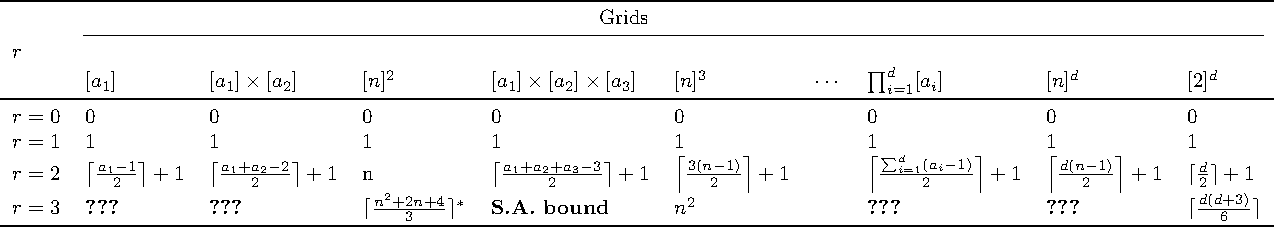
\includegraphics[width=\textwidth,origin=c]{tables/1/known_bounds.pdf}
\caption{A summary of known bootstrap percolation results for grids and the torus, $r \in \{0,1,2,3,d\}$.}
\label{tab:known_bounds}
\end{table} 

We end this introduction with the presentation of a delightful question about the cardinality of $2$-neighbor percolating sets on the two-dimensional lattice. The interested reader in encouraged to find a solution on their own; however, a proof of the result is presented at the beginning of the following section.
\begin{question}
Let $(n,n)$ represent the $n \times n$ lattice, given by $G = P_n \times P_n$. What is $m(n,n,2)$?
\end{question}

\section{Minimum percolating sets and bounds}

\subsection{Foundations}

Let us build some intuition for the behavior of percolating sets on the two-dimensional lattice. Figure \ref{fig:5x5x1} illustrates the percolation time-steps for an arbitrary initial infection on the graph $G=P_5 \times P_5$, where $r=2$. (In general, we shall refer to the $d$-dimensional lattice with sides $a_1, \dots, a_d$ as the $d$-tuple $(a_1, \dots, a_d)$. The standard notation is $\prod_{i=1}^d a_i$.) 

\begin{figure}[]
\centering
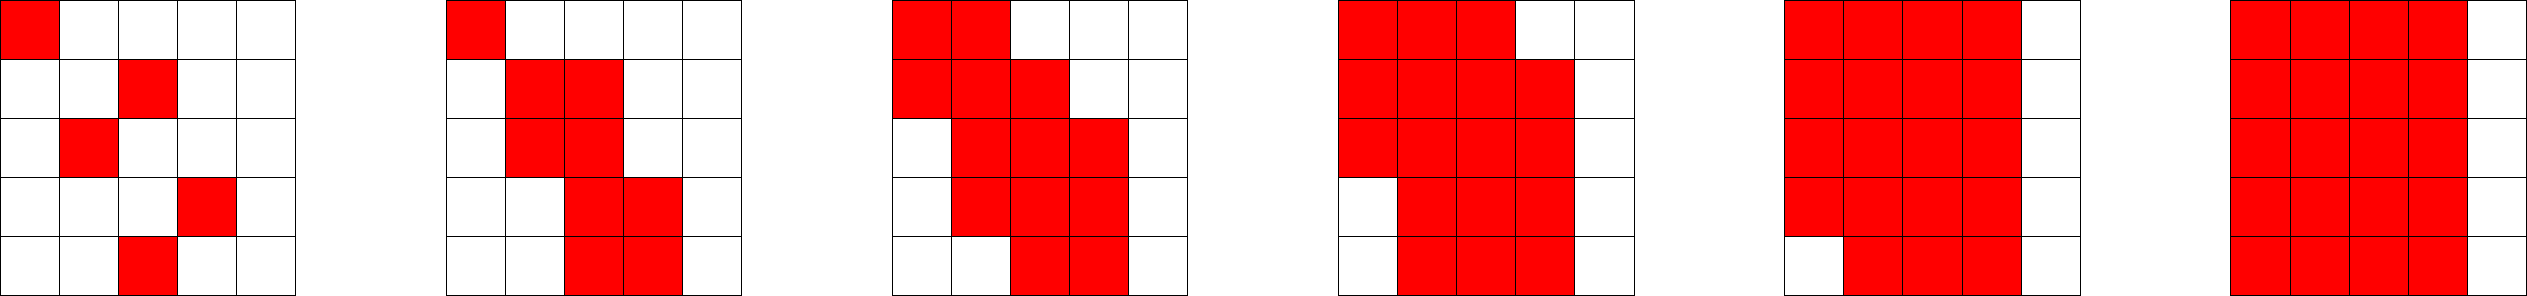
\includegraphics[width=\textwidth]{figures/1/5x5x1.pdf}
\caption{Percolation time-steps for an arbitrary initial infection on the $5 \times 5$ lattice, $r=2$.}
\label{fig:5x5x1}
\end{figure} 

Note that this configuration fails to infect the entire grid; that is, the initial infection is not lethal. Heuristically, this appears to be a consequence of the fact that infected cells are unable to access the healthy cells in the rightmost column. We might, therefore, hypothesize that an initial infection must somehow ``span" the entire lattice. A potential ``spanning" construction is illustrated in figure \ref{fig:5x5x1_improved}. Observe that at each time-step, the infection spreads out laterally from the initial diagonal. It is a simple exercise to verify that this construction is lethal on all $(n,n)$ grids for $r=2$. We also note that a similar construction is lethal on all $(n,m)$ grids for $r=2$ (figure \ref{fig:8x4x1}).

\begin{figure}[]
\centering
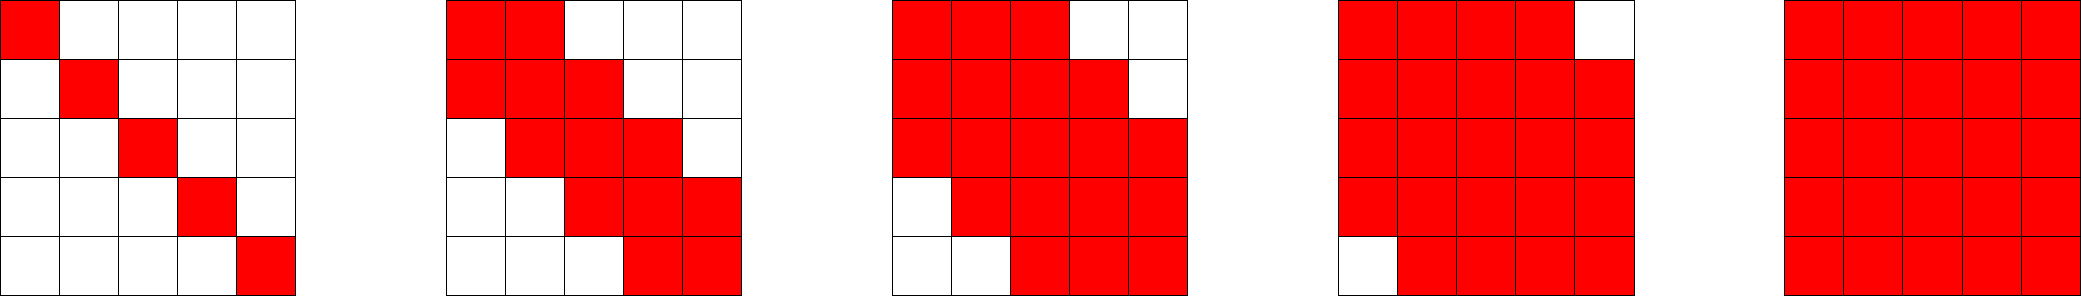
\includegraphics[width=\textwidth]{figures/1/5x5x1_improved.pdf}
\caption{Percolation time-steps for a ``spanning" initial infection on the $5 \times 5$ lattice, $r=2$.}
\label{fig:5x5x1_improved}
\end{figure} 

\begin{figure}[]
\centering
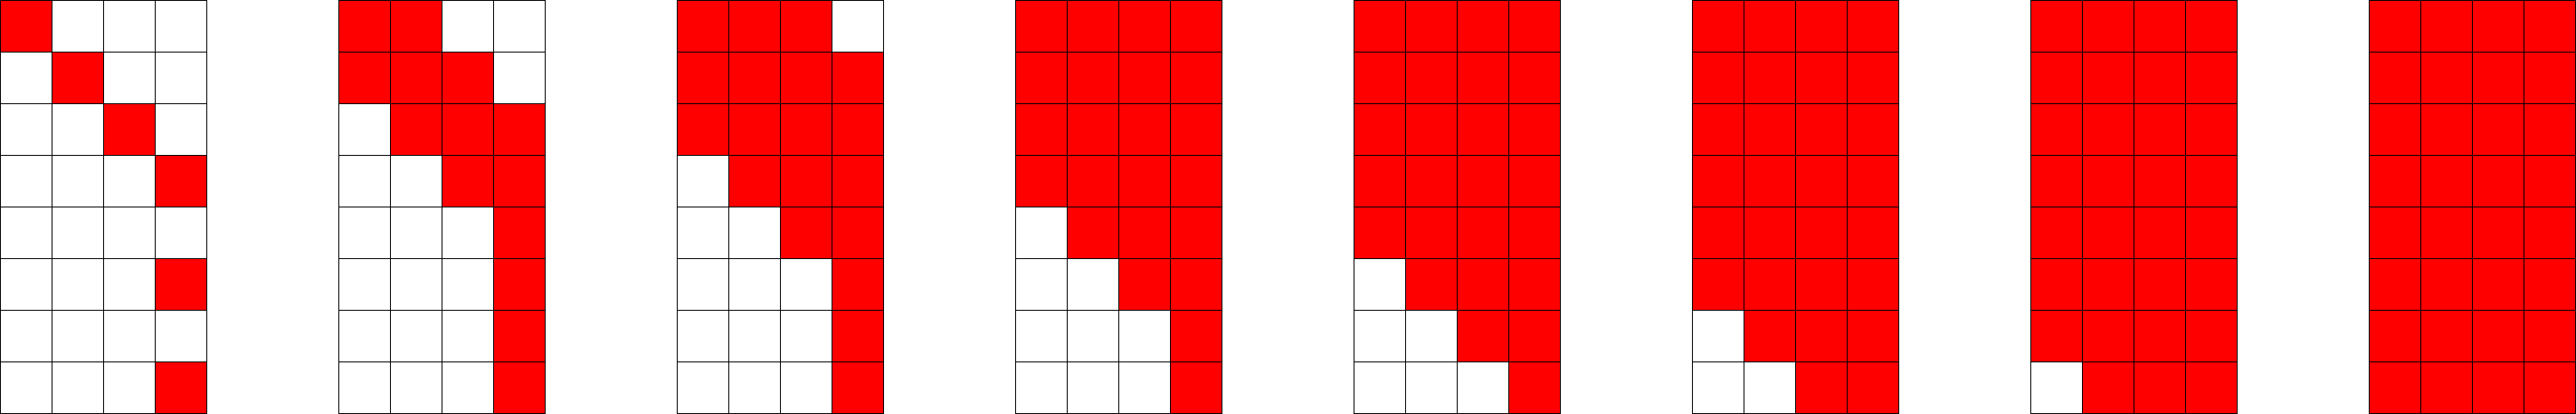
\includegraphics[width=\textwidth]{figures/1/8x4x1.pdf}
\caption{A lethal infection on the $8 \times 4$ lattice, $r=2$.}
\label{fig:8x4x1}
\end{figure} 

The $(n,n)$ construction can be generalized to any dimension. Specifically, we have:

\begin{prop}
\label{prop:nxn_lower_bound}
For all $n,d \geq 1$, 
$$m([n]^d, d) \leq n^{d-1}.$$
\end{prop}
This result has been known since at least Pete \cite{pete:1997}, although the particular constructions are difficult to render in general. The following proof (appearing in \cite{przykucki:2019}, but known in bootstrap percolation ``folklore" for much longer) elegantly shows that this bound is tight.

\begin{thm}
\label{thm:tight_perimeter}
For all $n,d \geq 1$, 
$$m([n]^d, d) = n^{d-1}.$$
\end{thm}

\begin{proof}
The upper bound follows from proposition \ref{prop:nxn_lower_bound}. The lower bound is given by a generalization of the famous ``perimeter argument". Suppose $d=2$ and consider an embedding of $G=[n]^d$ in the $n\times n$ grid. Let $A_0 \subseteq V(G)$ be a set of initially infected cells. We claim that the total perimeter of all infected regions in $G$ is monotonically decreasing as a function of the time-step $t$. Consider an arbitrary healthy cell $c$. In order for $c$ to become infected, at least two of its edges must abut infected cells. However, this implies that (upon infection of $c$) these edges are absorbed within the newly expanded infected region, thereby reducing the perimeter of infection by two. As $c$ contains at most two un-absorbed edges, the perimeter of infection cannot increase. 

Since a lethal set will infect the entire grid, and therefore have a final perimeter of infection of $4n$, it follows that the perimeter of infection of $A_0$ must be at least $4n$, and so $m([n]^2, 2) \geq n.$

The same argument generalizes nicely to higher dimensions. Simply observe that for a given hypercube cell to become infected, it must donate at least $d$ of its $2d$ hyperplane faces to the infected region, thereby at most maintaining the current $(d-1)$-perimeter of infection.
\end{proof}

We note that the perimeter argument extends directly to rectangular grids; however, the problem of obtaining tight constructions, should they exist, is largely unsolved and will be the main focus of this thesis. The following proposition, which we refer to informally as the \emph{surface area bound} or \emph{S.A. bound}, provides a lower bound on the size of lethal sets for $d$-dimensional rectangular grids where $r=d$.

\begin{prop}
\label{prop:SA_bound}
For $d \geq 1$ and $a_1, \dots, a_d \geq 1$,
$$m(a_1, \dots, a_d, d) \leq \frac{\sum_{i=1}^d \prod_{j \neq i} a_j}{d}.$$
\end{prop}

\begin{proof}
Observe that the expression
$$\frac{\sum_{i=1}^d \prod_{j \neq i} a_j}{d}$$
is precisely the high-dimensional perimeter of the grid graph $(a_1, \dots, a_d)$. The bound follows from the perimeter argument in theorem \ref{thm:tight_perimeter}. 
\end{proof}

In \{some chapter of this thesis\}, we will prove that this bound is tight in the case where $d=3$ and $d_1,d_2,d_3 \geq 8$. We fully expect that this bound can be incrementally diminished; however, we feel that such small improvements do not at this time justify the effort required to obtain additional constructions. 

In the remainder of this section, we shall present a number of additional bootstrap percolation results for different classes of grid graphs.

\subsection{Additional results}

Recall from the previous section that $m(n,n,2) = n$, where the tight construction for the lower bound is given by a diagonal infection expanding laterally outwards. In a paper by Balogh and Bollobas \cite{balogh:2006}, this result is generalized to all $d$-dimensional hypercubes $(a_1, \dots, a_d)$, $a_i \geq 1$. 

\begin{thm}
For $d \geq 1$ and $a_1, \dots, a_d \geq 1$, 
$$m(a_1, \dots, a_d, 2) = \ceil*{\frac{\sum_{i=1}^d (a_i-1)}{2}}+1.$$
\end{thm}

\begin{proof}
\end{proof}

As suggested by table \ref{tab:known_bounds}, general results become quite sparse for $r \notin \{2,d\}$. A nice result from Morrison and Noel resolves the question of $r=3$ for hypercubes $P_2^d$ of dimension $d \geq 3$. 

\begin{thm}
For $d \geq 3$ and $a_1 = \dots = a_d = 2$, 
$$m(a_1, \dots, a_d, 3) = \ceil*{\frac{d(d+3)}{6}}.$$
\end{thm}

\begin{proof}
\end{proof}

However, the issue of determining $m(a_1, \dots, a_d, r)$ is largely unresolved. Furthermore, good lower bounds for $r \neq d$ are conspicuously absent. 
\end{comment}
% ^^^ ONE GIANT COMMENT ^^^
% COMMENT
% COMMENT
% COMMENT
% COMMENT
% COMMENT



\chapter{Conceptual Tools}

As suggested in Chapter 1, it appears that lethal sets in grid graphs adhere to certain fixed rules. We examine these rules here, and explain why they are necessary and helpful for understanding the problem of bootstrap percolation.

\subsection{Integrality of bounds}

Not all grids have integral surface area bounds. We refer to such grids as \emph{non-divisibility cases}. The non-divisibility cases for three-dimensional grids where $r=3$ are illustrated in red in Table \ref{tab:integral_bounds}. 

As discussed in Chapter 1, percolation in non-divisible grids is inefficient in one of two ways: either $A_0$ contains adjacent vertices, or at some time-step $i$, there exists a vertex $v \in V \setminus A_i$ such that $N_{A_i}(v) > r$. 
% In the first case, the inefficiency is a consequence of two adjacent vertices in $A_0$; heuristically, we may view this as poor distribution of infection across the grid. In the second case, the inefficiency results from excessive infection in a particular region; a vertex is over-exposed. 

It is insightful to consider this behavior in the context of Theorem \ref{thm:torus_lb}. Instead of thinking of $m_{IH}$ at the number of edges between $I$ and $H$, we shall consider it to represent the perimeter, or surface area, of the initial infection $I$. 
%In particular, the existence of adjacent vertices in $A_0$ corresponds precisely to inequality in $m_{IH} \leq 2d|I| - 2(ab+bc+ca)$, where $2(ab+bc+ca)$ is the surface area of the grid. 
%In these cases, we are guaranteed the existence of at least one cell that is infected by more than $r$ neighbors. This is a direct consequence of the surface area argument; since the final surface area of infection is non-integral and surface area is non-increasing

\begin{table}[]
\centering
\begin{subfigure}{0.3\textwidth}
	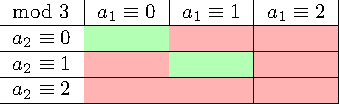
\includegraphics[width=\textwidth]{tables/1/integral_bounds_thickness_1.pdf}
	\caption{$a_3 \equiv 1 \pmod 3$}
	\label{tab:integral_bounds_a}
\end{subfigure} \hfill%
\begin{subfigure}{0.3\textwidth}
	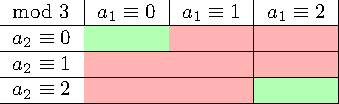
\includegraphics[width=\textwidth]{tables/1/integral_bounds_thickness_2.pdf}
	\caption{$a_3 \equiv 2 \pmod 3$}
	\label{tab:integral_bounds_b}
\end{subfigure} \hfill%
\begin{subfigure}{0.3\textwidth}
	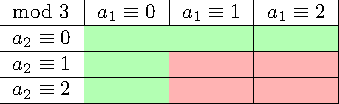
\includegraphics[width=\textwidth]{tables/1/integral_bounds_thickness_3.pdf}
	\caption{$a_3 \equiv 0 \pmod 3$}
	\label{tab:integral_bounds_c}
\end{subfigure}
\caption{Integrality of grids by congruence class. Green indicates integral surface area bound.}
\label{tab:integral_bounds}
\end{table} 

\subsection{A different characterization}

We shall find it useful to think about the problem of bootstrap percolation in terms of the graph induced by the set of uninfected vertices $V \setminus A_i$ at some time-step $t_i$. 

\subsection{Attributes of $G[V \setminus A]$}

No cycles, no paths between opposite faces. Reference to Benevides.

\subsection{The lower bound}

Let us reconsider the our proof of the lower bound in this new framework. 

\subsection{Surface area, optimality, trees, and components}

The surface area bound is not always integral. In cases where it is not, this sub-optimality can be traced to a particular time-step where an uninfected cell is infected by more than $r$ neighbors. The proof of the lower bound on the torus considers the number of components in $T[V \setminus A]$, as each such component necessarily collapses in on a vertex where this occurs. In the grid, this circumstance can be avoided by permitting components to abut the perimeter. What is the relationship here?

\subsection{The bipartition (and when to violate it)}

Discuss the heuristic of placing infections on one side of the bipartition and when this technique fails. 

\subsection{A potentially interesting proof framework}

A discussion on the broad structure of the proof of the lower bound on the torus as presented in Benevides. Note that this proof relies on a sequence of inequalities, and that two of these inequalities characterize precise conditions that are necessary for a set to be lethal. Discuss how the proof might change as a function of the dimension of the grid. 


\chapter{A Recursive Technique}

In the previous chapter, we examined some structures in grids that, if present, immediately guarantee lethality. Most significantly, we proved that lethal sets on mutually orthogonal walls of a grid are lethal on the entire grid. In the following sections, we leverage this result to show that certain configurations of fully infected sub-grids (which we shall call blocks) will cause the larger grid to become infected. Furthermore, we show that, if each of these smaller blocks is infected with a minimum lethal set, then the composite larger brick will also be infected with a minimum lethal set (barring some divisibility considerations).

\section{The Recursion}

The proof of this claim makes use of the so-called \emph{modified bootstrap process} in $[n]^d$, studied by Holroyd in \cite{holroyd2006metastability} and \cite{holroyd2003sharp}. This is a strengthened variation of the problem introduced in Chapter 1, whereby vertices in the $[n]^d$ grid become infected if and only if they are adjacent to infected vertices along edges in each of the $d$ directions. For example, in the $[n]^2$ grid, a vertex that sees infection in one of both the North/South and East/West directions will itself become infected, whereas a vertex with infected neighbors only to the East and West will not. 

In particular, the following lemma considers composite grids $[n]^d$ where each vertex $\mathbf{x} = (x_1, \dots, x_d) \in [n]^d$ is itself a smaller block. We prove that lethal sets on these grids can be built from the smaller lethal sets on each component block. 
% $[b_1] \times [b_2] \times \cdots \times [b_d]$ grid

\begin{figure}[]
\centering
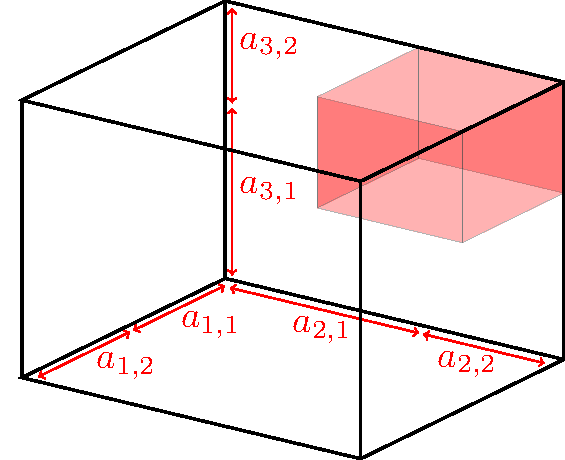
\includegraphics[width=0.4\textwidth]{figures/3/recursion.pdf}
\caption{A recursively constructed $[b_1] \times [b_2] \times [b_3]$ grid, for $n = 2$, $d = 3$.}
\label{fig:recursion}
\end{figure} 

\begin{lem}
\label{lem:recursion}
For $n,d \geq 1$, let $A = (a_{i,j})$ be a $d \times n$ matrix of positive integers, and let $b_i = \sum_{j=1}^n a_{i,j}$, for $1 \leq i \leq d$. Let $S$ be a lethal set under the modified process on $[n]^d$, and for each vertex $\mathbf{x} = (x_1, \dots, x_v) \in S$, let $T_{\mathbf{x}}$ be a lethal set on $\prod_{i=1}^d [a_{i,x_i}]$ under $d$-neighbor percolation. Then
$$m(b_1, \dots, b_d, d) \leq \sum_{\mathbf{x} \in S} |T_{\mathbf{x}}|.$$
\end{lem}

\begin{proof}
We sub-divide the $\prod_{i=1}^d [b_{i}]$ brick into smaller blocks by partitioning each of the $d$ axes into segments $a_{i,1}, a_{i,2}, \dots, a_{i,n}$, $1 \leq i \leq d$. Each block is given by a unique product of these segments, and represented by a vector $\mathbf{x} = (x_1, \dots, x_d) \in [n]^d$. Formally, for each such $\mathbf{x}$, let $G_{\mathbf{x}}$ be the block with vertex set
$$\prod_{i=1}^d \left\{1+ \sum_{j=1}^{x_i -1}a_{i,j}, \dots, \sum_{j=1}^{x_i}a_{i,j} \right\},$$
and edges between vertices that differ by one in exactly one coordinate. Figure \ref{fig:recursion} illustrates the block $G_{\mathbf{x}}$ for $\mathbf{x} = (1,2,2) \in [2]^3$. Observe that $G_{\mathbf{x}}$ is isomorphic to $\prod_{i=1}^d [a_{i,x_i}]$.

For each $\mathbf{x} \in S$, let $A_{\mathbf{x}}$ be the vertices of $G_{\mathbf{x}}$ corresponding to the vertices of $T_{\mathbf{x}}$ under isomorphism from $\prod_{i=1}^d [a_{i,x_i}]$ to $G_{\mathbf{x}}$, and let $A_0 = \cup A_{\mathbf{x}}$. Observe that $|A_0| = \sum_{\mathbf{x} \in S} |T_{\mathbf{x}}|$. We show that $A_0$ is lethal on $\prod_{i=1}^d [b_{i}]$.

By the definition of $T_{\mathbf{x}}$, for each $\mathbf{x} \in S$, $A_{\mathbf{x}}$ is lethal on $G_{\mathbf{x}}$. Run the $d$-neighbor process until all blocks $G_{\mathbf{x}}$ are fully infected. We claim that this is sufficient to infect all remaining vertices of $\prod_{i=1}^d [b_{i}]$. Consider the remaining blocks $G_{\mathbf{x}}$, for $\mathbf{x} \in [n]^d \setminus S$. Since $S$ is lethal under the modified process, at some point in the infection process each $G_{\mathbf{x}}$ is adjacent to fully infected blocks in all $d$ directions. 
%In particular, if we consider expanding out the faces of $G_{\mathbf{x}}$ towards these infected blocks, the resulting cube has $d$ fully infected faces that share a common corner. 
By Corollary \ref{cor:three_walls}, this is sufficient to infect all the vertices of $G_{\mathbf{x}}$. Repeating this process on each uninfected region of $\prod_{i=1}^d [b_{i}]$ (as they are exposed under the modified process) ultimately results in all vertices becoming infected. This completes the proof. 
\end{proof}

% Corollary that shows the recursion produces tight bounds on the size of lethal sets, IF all of the constituent blocks are divisibility cases
We note that although the lemma above is true in full generality, we only apply it in the particular case where $n=2$ and $d=3$. The following corollary proves that the bound in Lemma \ref{lem:recursion} is tight for $n=2$ and $d=3$, provided that the lethal sets on at least three of the constituent blocks are perfect. 

\begin{cor}
\label{cor:recursion}
Let $A=(a_{i,j})$ be a $3 \times 2$ matrix of positive integers, and let $b_i = a_{i,1} + a_{i,2}$ for all $1 \leq i \leq 3$. Then $m(b_1, b_2, b_3, 3)$ is at most
$$m(a_{1,1}, a_{2,1}, a_{3,1}, 3) +  m(a_{1,2}, a_{2,2}, a_{3,1}, 3) + m(a_{1,2}, a_{2,1}, a_{3,2}, 3) + m(a_{1,1}, a_{2,2}, a_{3,2}, 3).$$
Furthermore, this bound is tight if at least three of $\{(a_{1,1}, a_{2,1}, a_{3,1})$, $(a_{1,2}, a_{2,2}, a_{3,1})$, $(a_{1,2}, a_{2,1}, a_{3,2})$, $(a_{1,1}, a_{2,2}, a_{3,2})\}$ are perfect. 
\end{cor}

\begin{proof}
The upper bound on $m(b_1, b_2, b_3, 3)$ is a direct consequence of Lemma \ref{lem:recursion}, since the set $\{(1,1,1), (2,2,1), (2,1,2), (1,2,2)\}$ of vertices is lethal under the modified process on $[2]^3$. 

If all constituent grids are perfect, then:  
\begin{align*}
&m(a_{1,1}, a_{2,1}, a_{3,1}, 3) +  m(a_{1,2}, a_{2,2}, a_{3,1}, 3) + m(a_{1,2}, a_{2,1}, a_{3,2}, 3) + m(a_{1,1}, a_{2,2}, a_{3,2}, 3) \\[10pt]
&= \frac{a_{1,1}a_{2,1} + a_{2,1}a_{3,1} + a_{3,1}a_{1,1}}{3} + \frac{a_{1,2}a_{2,2} + a_{2,2}a_{3,1} + a_{3,1}a_{1,2}}{3} \\
&\qquad\qquad\qquad\qquad\qquad\qquad\quad + \frac{a_{1,2}a_{2,1} + a_{2,1}a_{3,2} + a_{3,2}a_{2,1}}{3} + \frac{a_{1,1}a_{2,2} + a_{2,2}a_{3,2} + a_{3,2}a_{1,1}}{3} \\[10pt]
&= \frac{(a_{1,1} + a_{1,2})(a_{2,1} + a_{2,2}) + (a_{2,1} + a_{2,2})(a_{3,1} + a_{3,2}) + (a_{3,1} + a_{3,2})(a_{1,1} + a_{1,2})}{3} \\[10pt]
&= \frac{b_1b_2+b_2b_3+b_3b_1}{3}.
\end{align*}
Similarly, suppose, without loss of generality, that $(a_{1,1}, a_{2,1}, a_{3,1})$ is optimal and the remaining grids are perfect. Then:
\begin{align*}
&m(a_{1,1}, a_{2,1}, a_{3,1}, 3) +  m(a_{1,2}, a_{2,2}, a_{3,1}, 3) + m(a_{1,2}, a_{2,1}, a_{3,2}, 3) + m(a_{1,1}, a_{2,2}, a_{3,2}, 3) \\[10pt]
&= \ceil*{\frac{a_{1,1}a_{2,1} + a_{2,1}a_{3,1} + a_{3,1}a_{1,1}}{3}} + \frac{a_{1,2}a_{2,2} + a_{2,2}a_{3,1} + a_{3,1}a_{1,2}}{3} \\
&\qquad\qquad\qquad\qquad\qquad\qquad\quad + \frac{a_{1,2}a_{2,1} + a_{2,1}a_{3,2} + a_{3,2}a_{2,1}}{3} + \frac{a_{1,1}a_{2,2} + a_{2,2}a_{3,2} + a_{3,2}a_{1,1}}{3} \\[10pt]
&= \ceil*{\frac{(a_{1,1} + a_{1,2})(a_{2,1} + a_{2,2}) + (a_{2,1} + a_{2,2})(a_{3,1} + a_{3,2}) + (a_{3,1} + a_{3,2})(a_{1,1} + a_{1,2})}{3}} \\[10pt]
&= \ceil*{\frac{b_1b_2+b_2b_3+b_3b_1}{3}}.
\end{align*}
In both cases, we obtain an upper bound on $m(b_1, b_2, b_3, 3)$ matching the lower surface area bound. This completes the proof. 
\end{proof}

\section{Building Blocks}

\begin{table}[]
\centering
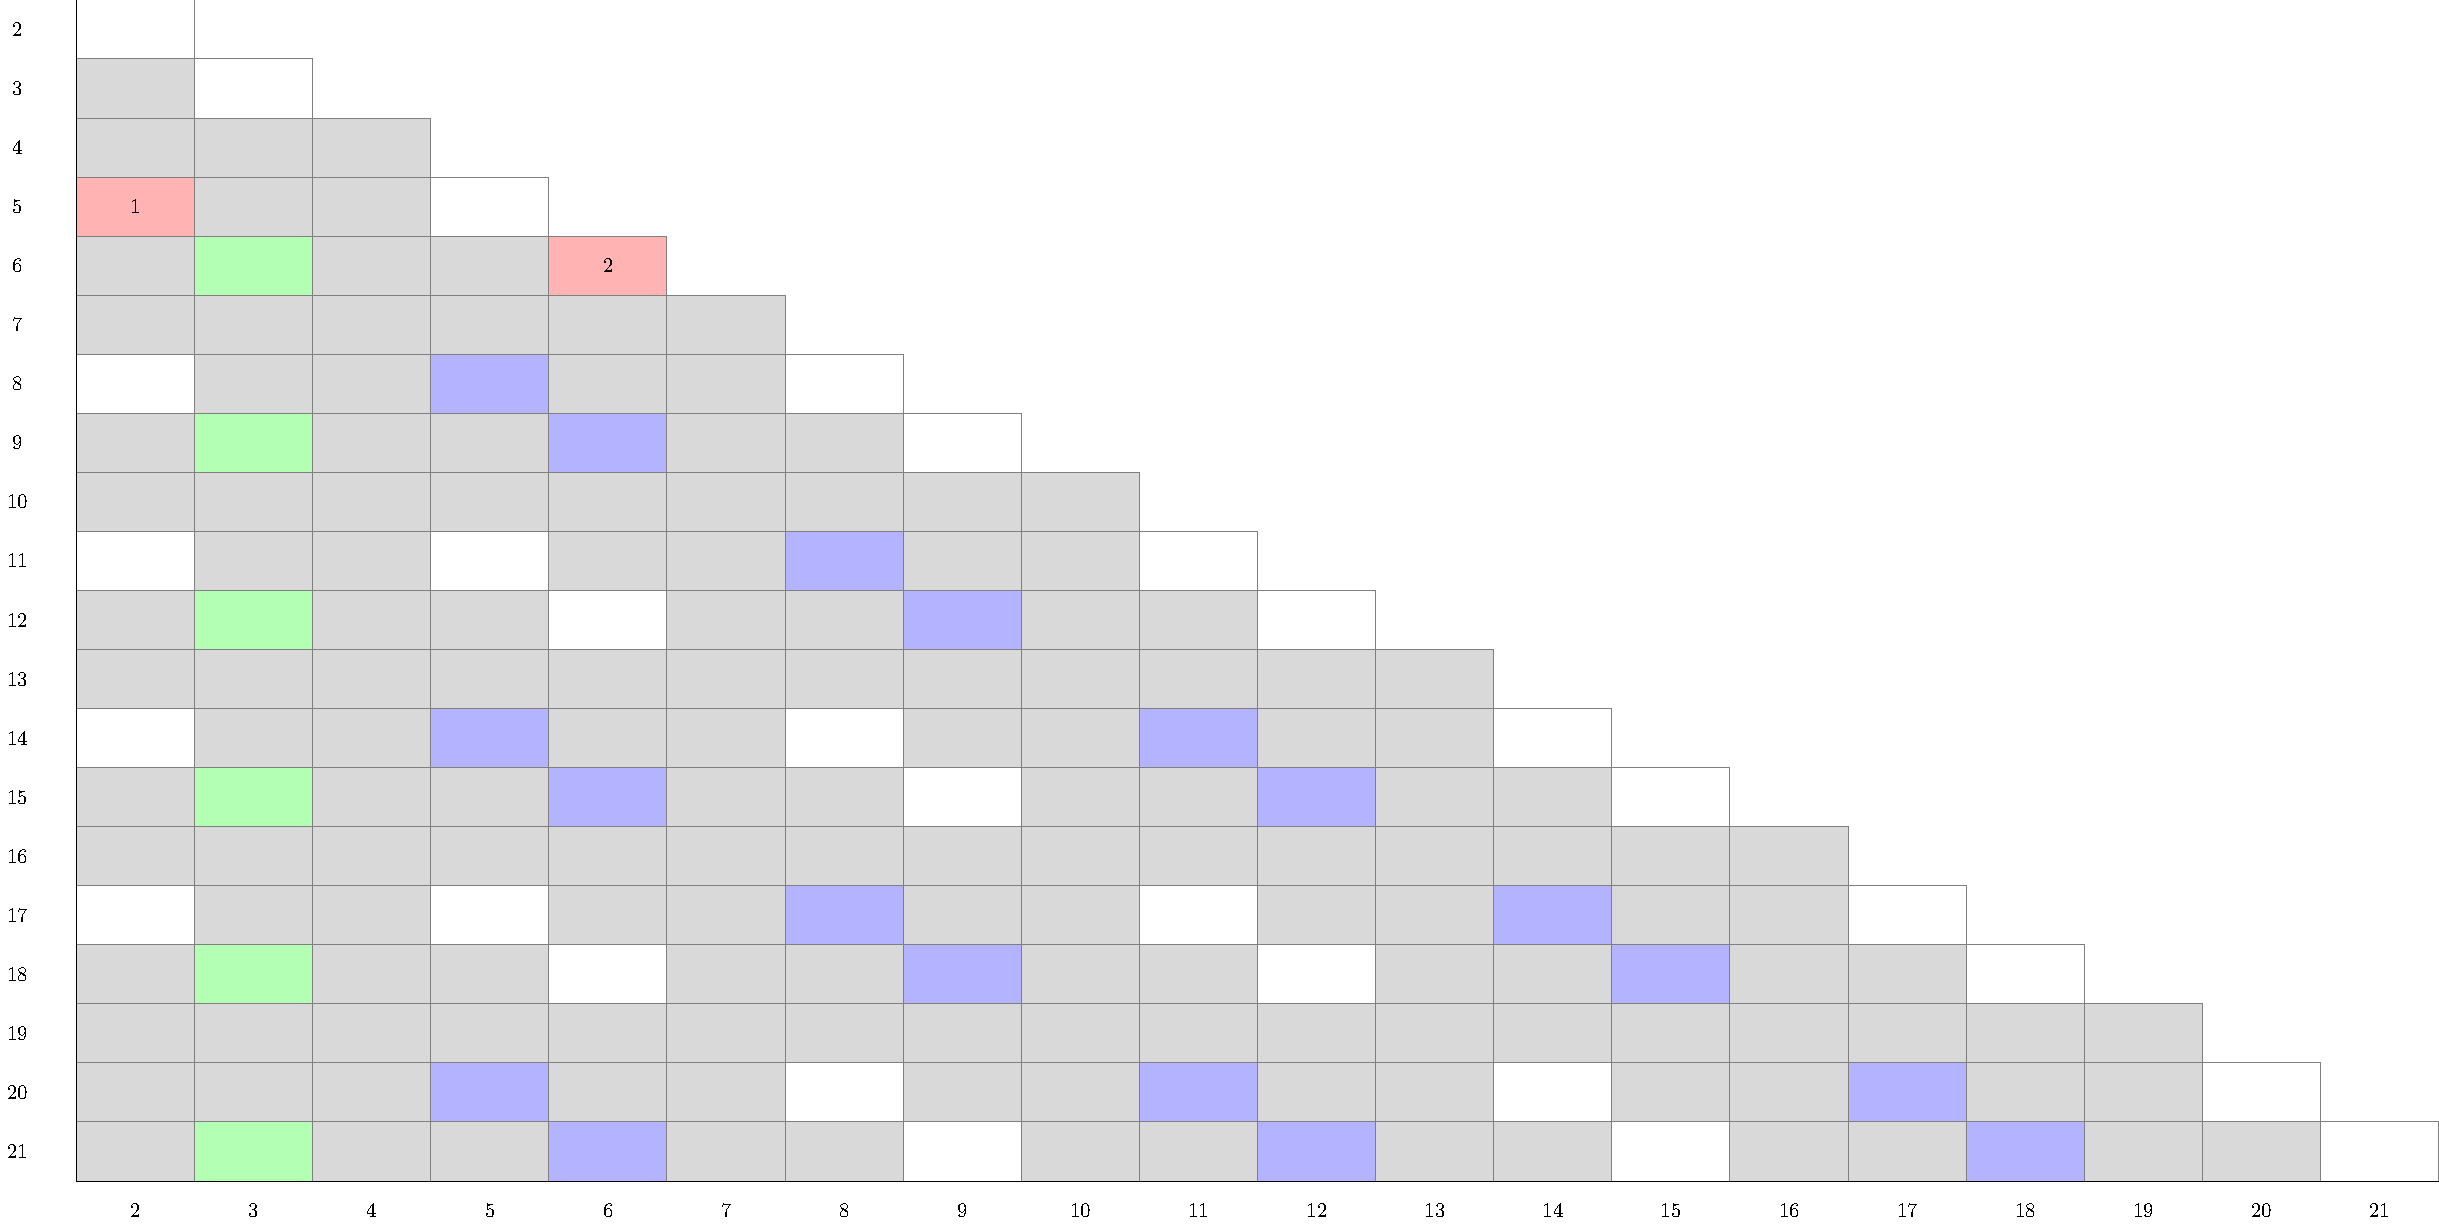
\includegraphics[width=\textwidth]{tables/2/thickness_2.pdf}
\caption{Thickness 2 constructions used in the proof of Theorem \ref{thm:main_result}. Blue and green cells represent infinite families of constructions. Red cells are individual constructions. Divisibility cases are white and non-divisibility cases are gray.}
\label{tab:integral_bounds_2}
\end{table} 

\begin{table}[]
\centering
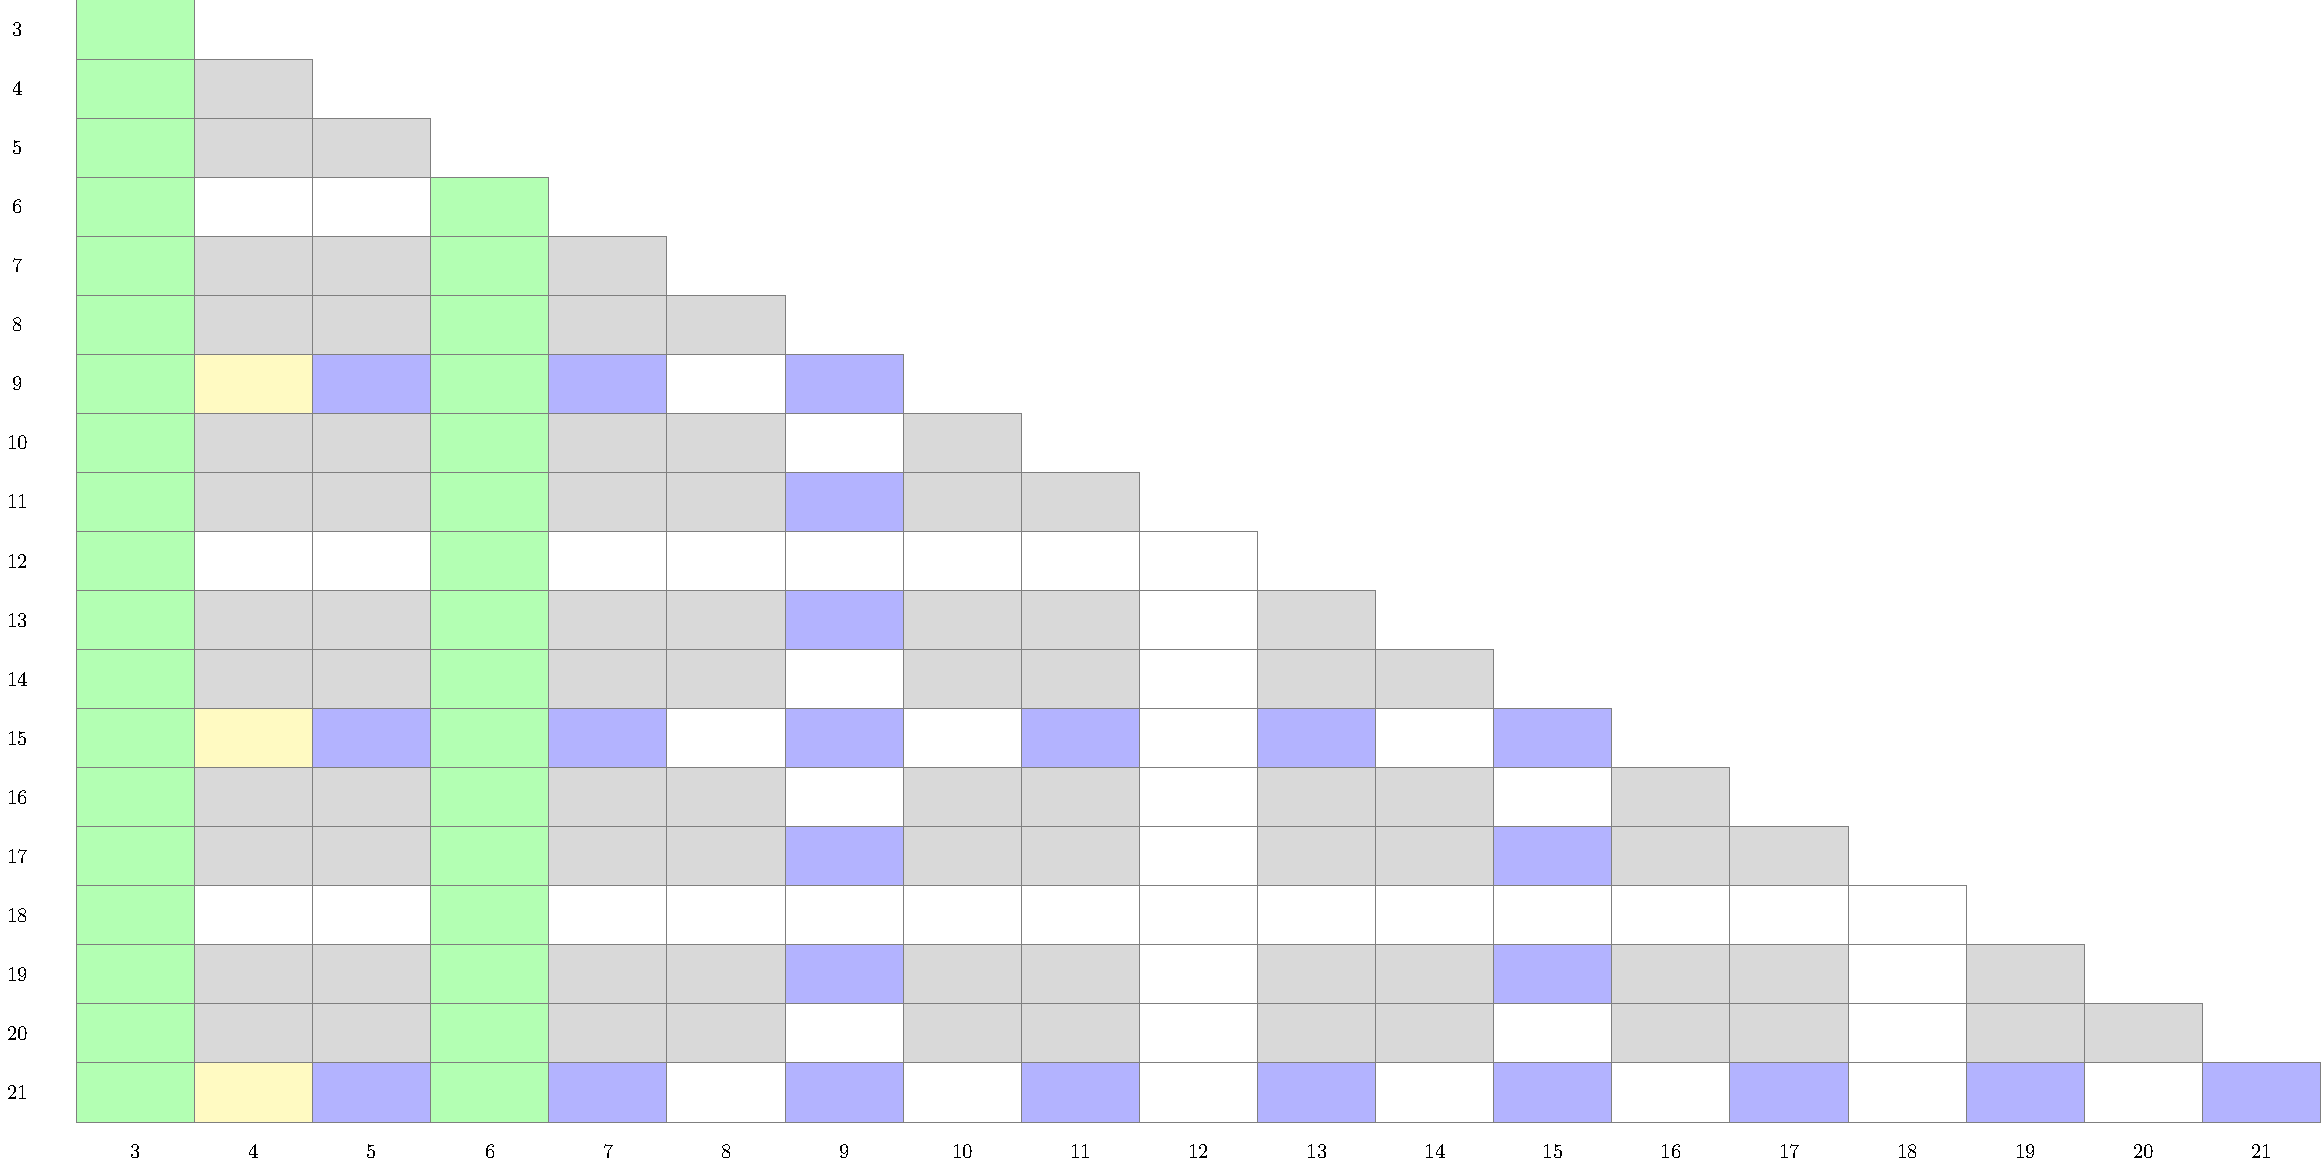
\includegraphics[width=\textwidth]{tables/2/thickness_3.pdf}
\caption{Thickness 3 constructions used in the proof of Theorem \ref{thm:main_result}. Blue, green and yellow cells represent infinite families of constructions. Divisibility cases are white and non-divisibility cases are gray.}
\label{tab:integral_bounds_3}
\end{table} 

\begin{table}[]
\centering
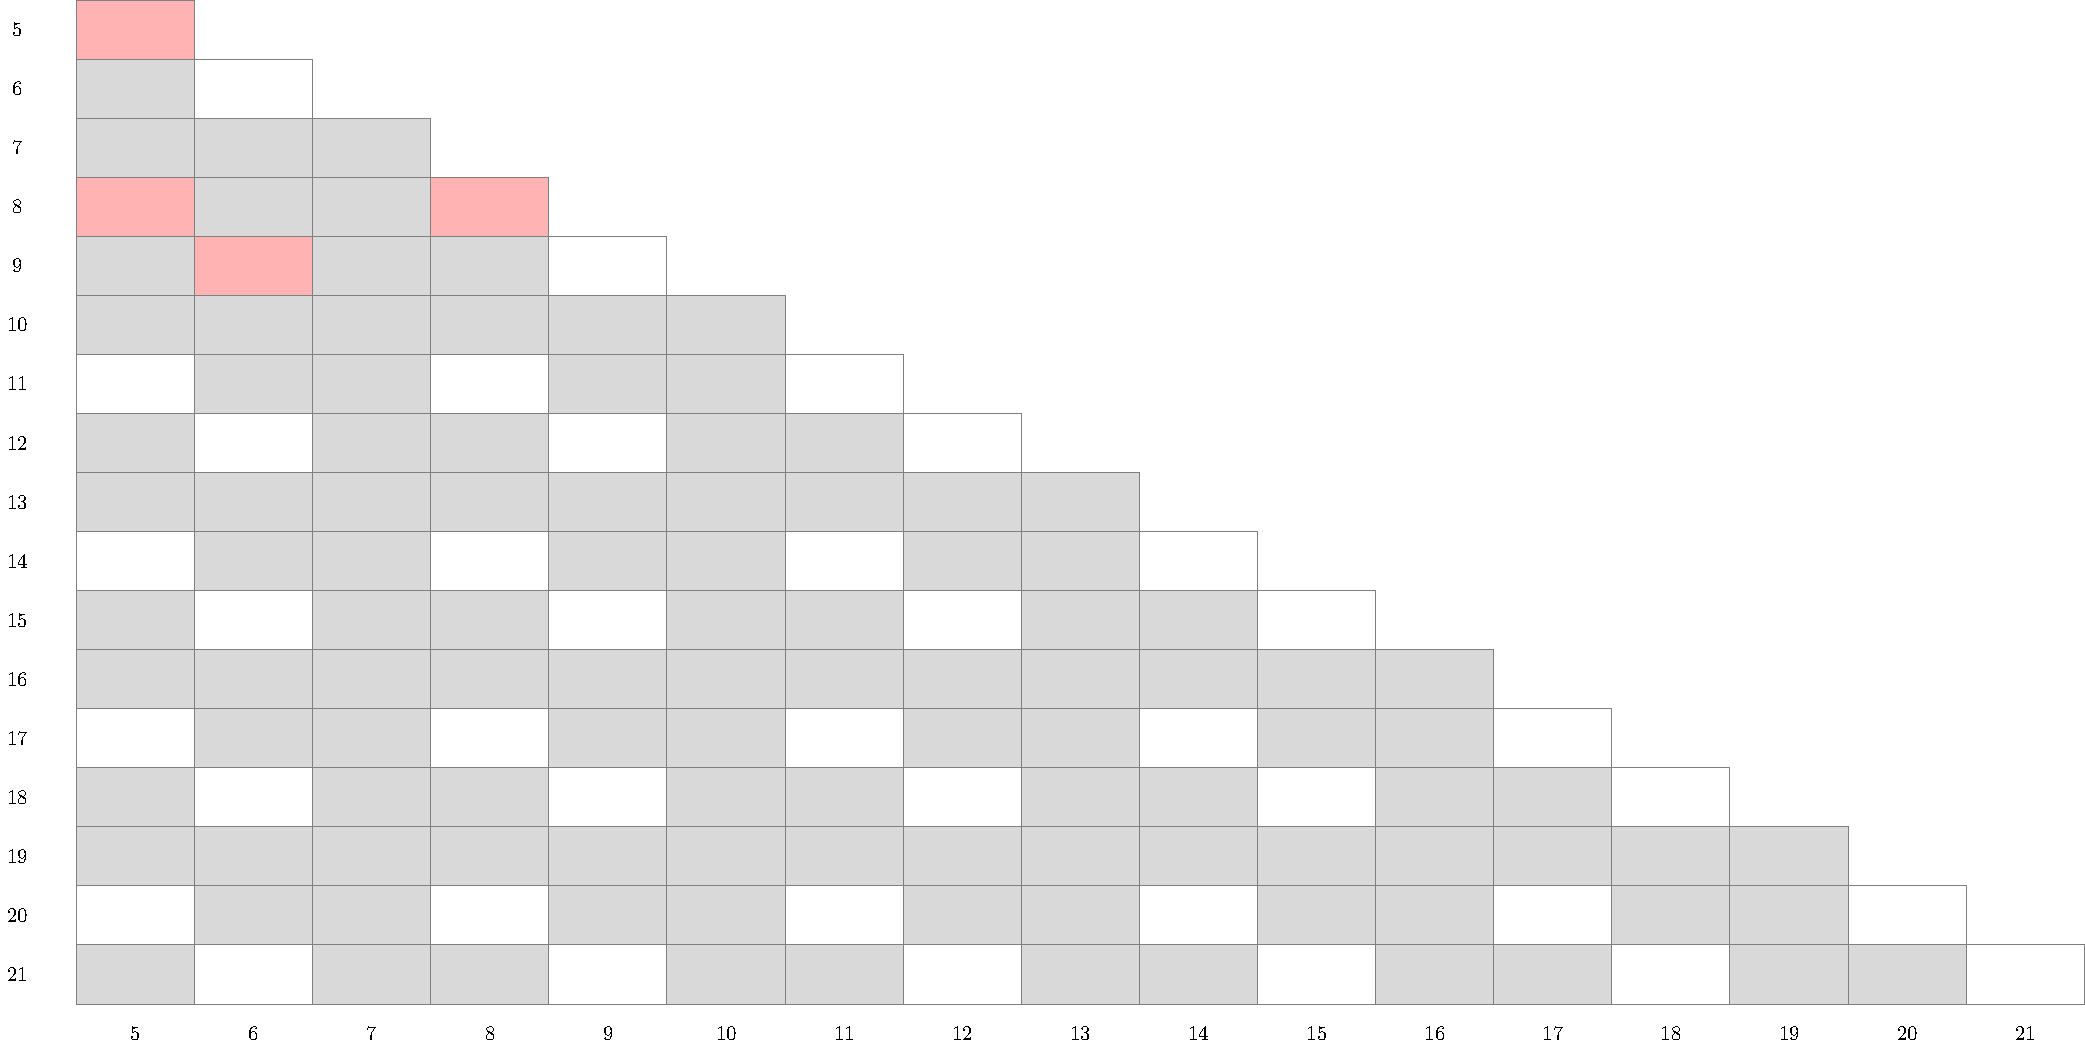
\includegraphics[width=\textwidth]{tables/2/thickness_5.pdf}
\caption{Thickness 5 constructions used in the proof of Theorem \ref{thm:main_result}. Red cells are individual constructions. Divisibility cases are white and non-divisibility cases are gray.}
\label{tab:integral_bounds_5}
\end{table}

% Handle the divisibility cases, and note that certain augmentations to the recursion allow us to obtain non-divisible optimal grids, if we are cautious with regard to the pieces we use.
Corollary \ref{cor:recursion} provides a prescriptive method for constructing optimal and perfect lethal sets recursively, provided the existence of sufficiently many small building blocks. In the following chapter, we use this technique to obtain perfect lethal sets on all $G(b_1,b_2,b_3)$ grids, for $b_1,b_2,b_3 \geq 5$, and optimal lethal sets on all $G(b_1,b_2,b_3)$ grids, for $b_1,b_2,b_3 \geq 11$. To facilitate this process, we first summarize some useful families of lethal sets, as well as particular applications of Corollary \ref{cor:recursion} that hold for general grids. We note that the existence of these families is predicated on a number of constructions, which are analyzed in greater detail in Chapter 6. A summary of the lethal sets obtained in Propositions \ref{prop:3x3xk} -- \ref{prop:purina} is illustrated in Tables \ref{tab:integral_bounds_2}, \ref{tab:integral_bounds_3}, and \ref{tab:integral_bounds_5})

\begin{prop}
\label{prop:3x3xk}
For all $k \geq 1$ such that $k \neq 2$, $(3,3,k)$ is perfect.
\end{prop}

\begin{proof}
We obtain $(3,3,k)$ for $k \equiv 0 \pmod 2$ and $k > 2$ from Construction \ref{con:3x3xeven}, and $(3,3,k)$ for $k \equiv 1 \pmod 2$ and $k > 2$ from Construction \ref{con:3xaxb}. The case of $(3,3,1)$ is given in Benevides et al. \cite{benevides:2021}, and reproduced as Construction \ref{con:purina}.
\end{proof}

\begin{prop}
\label{prop:2x3xk_0}
For all $k \equiv 0 \pmod 6$ such that $k>3$, $(k,2,3)$ is perfect.
\end{prop}

\begin{proof}
We obtain $(k,2,3)$ for $k \equiv 0 \pmod 6$ and $k > 3$ from Construction \ref{con:3x2xa_mod6}. 
\end{proof}

\begin{prop}
\label{prop:3x6xk}
For all $k \geq 2$, $(3,6,k)$ is perfect.
\end{prop}

\begin{proof}
We obtain $(3,6,k)$ for $k \equiv 0 \pmod 2$ and $k \geq 4$ from Construction \ref{con:3x6xeven}, and $(3,6,k)$ for $k \equiv 1 \pmod 2$ and $k \geq 5$ from Construction \ref{con:3xaxb}. The remaining tuples $(3,6,2)$ and $(3,6,3)$ are obtained from Propositions \ref{prop:2x3xk_0} and \ref{prop:3x3xk}.
\end{proof}

\begin{prop}
\label{prop:thickness_3_2d_family}
For all $k \equiv 3 \pmod 6$ and $l \equiv 1 \pmod 2$ such that $l >1$, $(3,k,l)$ is perfect.
\end{prop}

\begin{proof}
We obtain such tuples from Construction \ref{con:3xaxb}.
\end{proof}

\begin{prop}
\label{prop:thickness_2_2d_family}
For all $k,l \in \{0,2,3,5\} \pmod 6$ such that $k \not\equiv l \pmod 6$, $k \equiv l \pmod 3$, and $k,l > 2$, $(k,l,2)$ is perfect.
\end{prop}

\begin{proof}
We obtain $(k,l,2)$ for $k,l \in \{2,5\} \pmod 6$ such that $k \not\equiv l \pmod 6$ and $k,l > 2$ from Construction \ref{con:2x2x5_mod6}. We obtain $(k,l,2)$ for $k,l \in \{0,3\} \pmod 6$ such that $k \not\equiv l \pmod 6$ and $k,l \geq 6$ from Construction \ref{con:2x3x0_mod6}. The remaining tuples are of the form $(k,3,2)$ for $k \equiv 0 \pmod 6$ and these are obtained from Construction \ref{con:3x2xa_mod6}.
\end{proof}

\begin{prop}
\label{prop:thickness_3_width_4}
For all $k \equiv 3 \pmod 6$, $(k,4,3)$ is perfect.
\end{prop}

\begin{proof}
We obtain $(k,4,3)$ for $k \equiv 3 \pmod 6$ and $k \geq 9$ from Construction \ref{con:3x4xa}. The case of $(4,3,3)$ is given by Proposition \ref{prop:3x3xk}.
\end{proof}

\begin{prop}
\label{prop:2x3xk_3}
For all $k \equiv 3 \pmod 6$ such that $k>3$, $(k,2,3)$ is perfect.
\end{prop}

\begin{proof}
We obtain $(k,2,3)$ for $k \equiv 3 \pmod 6$ and $k > 3$ from Construction \ref{con:3x2x(3mod6)}.
\end{proof}

\begin{prop}
\label{prop:purina}
For all $k \geq 1$, $(2^k-1,2^k-1,1)$ is perfect.
\end{prop}

\begin{proof}
The construction for such tuples is presented in \cite{benevides:2021} and reproduced as Construction \ref{con:purina}.
\end{proof}

Combining the above propositions with Corollary \ref{cor:recursion}, we are able to obtain the following lemmas.

\begin{lem}
\label{lem:plus_333}
Suppose $(b_1, b_2, b_3)$ is optimal and $b_1,b_2,b_3 \neq 2$. Then $(b_1+3, b_2+3, b_3+3)$ is optimal. 
\end{lem}

\begin{proof}
By Proposition \ref{prop:3x3xk}, each of $(b_1,3,3), (3,b_2,3),(3,3,b_3)$ is perfect. Therefore, by Corollary \ref{cor:recursion}, 
%$$m(b_1+3, b_2+3, b_3+3, 3) = m(b_1,b_2,b_3,3) + m(b_1,3,3,3) + m(3,b_2,3,3) + m(3,3,b_3,3),$$
$(b_1+3, b_2+3, b_3+3)$ is optimal.
\end{proof}

\begin{lem}
\label{lem:plus_336}
Suppose $(b_1, b_2, b_3)$ is optimal, $b_1,b_2 \geq 2$, and $b_3 \neq 2$. Then $(b_1+3, b_2+3, b_3+6)$ is optimal. 
\end{lem}

\begin{proof}
By assumption, $(b_1,b_2,b_3)$ is optimal. Both of $(b_1,3,6)$ and $(3,b_2,6)$ are perfect by Proposition \ref{prop:3x6xk}. By Proposition \ref{prop:3x3xk}, $(3,3,b_3)$ is perfect. Therefore, by Corollary \ref{cor:recursion}, 
%$$m(b_1+3, b_2+3, b_3+6, 3) = m(b_1,b_2,b_3,3) + m(b_1,3,6,3) + m(3,b_2,6,3) + m(3,3,b_3,3),$$
$(b_1+3, b_2+3, b_3+6)$ is optimal.
\end{proof}

In the following chapter, we shall see that the existence of the perfect lethal sets on the families of grids presented above, coupled with Corollary \ref{cor:recursion}, is enough to prove Theorem \ref{thm:main_result}. Speaking analogically, Propositions \ref{prop:3x3xk} -- \ref{prop:purina} (and the individual constructions in Appendix A) are the atomic pieces required to generate all molecular lethal sets. It should be noted that the atomic constructions used in this thesis are in no way special; there is likely a simpler combination of constructed lethal sets that also generates all grids $G(a_1,a_2,a_3)$, for $a_1,a_2,a_3 \geq 11$. These are simply the constructions that we were able to obtain. It would be interesting to determine, in general, the smallest number of constructed lethal sets required to build all other lethal sets in $d$-dimensional grids using Corollary \ref{cor:recursion}. 

% Example of the recursion on a small grid and discussion re: the strategies for analyzing percolating sets

%\section{Examples and Notation}

% Discuss that the recursion works by assembling any set of compatible n^2 blocks, although it is very rare that it is necessary to use more than 4. 
% Talk about the component pieces necessary to assemble a brick of size (a,b,c).

% Should we talk about the broad behavior of percolating sets?
%\section{Regional vs. Temporal Infections}

% COMMENT
% COMMENT
% COMMENT

\begin{comment}

\section{The Three Walls Lemma}

\begin{lem}
\label{lem:walls}
Let $S$ be an infected set on $G = \prod_{i=1}^d [a_i]$. Let $\overline{S} = V(G) \setminus S$, and let $H = G[\overline{S}]$ be the subgraph of $G$ induced by $\overline{S}$. For $1 \leq k \leq a_j$, let $F_{j,k} = \prod_{i=1}^{j-1} [a_i] \times \{k\} \times \prod_{i=j+1}^{d} [a_i]$ be the $k$th face of $G$ in the $j$th dimension. If $H$ does not contain a path between $F_{j,1}$ and $F_{j,a_j}$, for all $1 \leq j \leq d$, then $S$ is lethal on $G$ under $d$-neighbor percolation.
\end{lem}

\begin{proof}
We proceed by induction on $|V(H)| = \prod_{i=1}^d a_i - |S|$. If $|V(H)| = 0$, then all vertices of $G$ are infected and we are done. Suppose $|V(H)| > 0$, and consider a connected component $Y$ of $H$. By hypothesis, for all $j \in [d]$, either $V(Y) \cap F_{j,1} = \emptyset$ or $V(Y) \cap F_{j,a_j} = \emptyset$ (or both). Suppose, without loss of generality, that $V(Y) \cap F_{j,a_j} = \emptyset$.
%Since $V(H) > 0$, there exists a $k_j < a_j$ such that $V(Y) \cap F_{j,k_j}$ is non-empty. 
For each $j \in [d]$, let $x_j$ be the maximum value such that $V(Y) \cap F_{j,x_j}$ is non-empty. Note that such an $x_j$ must exist since $|V(H)| > 0$. 

Consider the vertex $\vec{x} = (x_1, \dots, x_d) \in V(Y)$, and observe that 
$$\{\bigcup_{j \in [d]} F_{j,x_j+1}\} \cap  V(Y) = \emptyset.$$
In particular, note that $(x_1+1, x_2, \dots, x_d), \dots, (x_1, \dots, x_d+1) \in N_S(\vec{x})$. Therefore, $\vec{x}$ becomes infected. Furthermore, since $|V(H) \setminus \{\vec{x}\}| < |V(H)|$, the resulting graph percolates by induction. This completes the proof.
\end{proof}

\begin{cor}
\label{cor:walls}
Let $G$ be the grid graph $\prod_{i=1}^d [a_i]$. For each $j \in [d]$ and some $1 \leq k \leq a_j$, let 
$$M = \bigcup_{j,k} F_{j,k}$$
be a subset of the vertices of $G$ formed by the union of mutually orthogonal faces. If a set $S$ is lethal on $M$, then it is lethal on $G$. 
%Let $G$ be the grid graph $(a,b,c)$. If a set $A$ is lethal on three mutually orthogonal faces of $G$, then $A$ is lethal on $G$.
\end{cor}

\begin{proof}
Since $S$ is lethal on $M$, there exists a time $t$ where $M \subseteq A_t$. Therefore, for all $j \in [d]$, the graph $G[\overline{A_t}]$ cannot contain a path between $F_{j,1}$ and $F_{j,a_j}$. By Lemma \ref{lem:walls}, $S$ is lethal on $G$. 
%Let $X, Y, Z$ be three mutually orthogonal faces of $G$. By hypothesis, $X \cup Y \cup Z \subseteq A_t$ for some time $t$. Therefore, the graph $H = G[\overline{A_t}]$ cannot contain a path between vertices on orthogonal faces of $G$. By lemma \ref{lem:walls}, $G$ percolates.
\end{proof}

Corollary \ref{cor:walls} provides a general characterization of lethal sets on $d$-dimensional grids in terms of their $(d-1)$-dimensional faces, provided these faces are mutually orthogonal. Here, we return to the notion first introduced in Chapter 1 of the capacity of a lethal set to ``span" a grid. In particular, we see that the set in Figure \ref{fig:two_infections_a} is comprised of lethal sets on the two one-dimensional orthogonal faces $F_{1,1}$ and $F_{2,1}$ of $[10]^2$. In this regard, the problem of obtaining perfect $d$-neighbor lethal sets on $d$-dimensional grids is reduced to the problem of determining a ``good" union $M$ of mutually orthogonal $(d-1)$-dimensional faces. 
%Once found, each face in $M$ can itself be infected by this same recursive process. 
In Chapter \{CONSTRUCTIONS\}, we apply this idea to obtain an infinite family of three-dimensional grids from three orthogonal two-dimensional faces. However, we caution that the challenge of determining a ``good" union $M$ is non-trivial in general.

The following corollary (taken as a particular instance of Corollary \ref{cor:walls}) will be useful in our discussion of lethal sets on three-dimensional grids $(a_1,a_2,a_3)$. 

\begin{cor}
\label{cor:three_walls}
Let $G$ be the grid graph $(a_1,a_2,a_3)$. If a set $S$ is lethal on $F_{1,1} \cup F_{2,1} \cup F_{3,1}$, then $S$ is lethal on $G$.
\end{cor}

\begin{proof}
By hypothesis, $S$ is lethal on $F_{1,1} \cup F_{2,1} \cup F_{3,1}$. Therefore, there exists some time $t$ for which $F_{1,1} \cup F_{2,1} \cup F_{3,1} \subseteq A_t$, and so $G[\overline{A_t}]$ satisfies the conditions of Lemma \ref{lem:walls}. We conclude that $S$ is lethal on $G$.
\end{proof}

\section{Manifolds}

We refer to unions $M$ of perpendicular faces as manifolds. As suggested in the previous section, there are a wide variety of possible manifold structures for a given grid. We highlight two particular structures in Figure \ref{fig:manifold_types}. The following two lemmas show that it is possible to obtain perfect lethal sets on these structures from existing perfect sets on grids of thickness one. 

%As discussed above, the capacity to generate ``good" sets $M$ is critical for building perfect lethal sets recursively. QUESTION: If we apply the above recursive process to faces, do the bounds match up? We shall examine the particular case of orthogonal faces on three-dimensional grids.

% I KNOW THIS ISN'T QUITE RIGHT. 
% The idea is that the three faces minus their pairwise intersections, plus their complete intersection matches the lower bound on (a,b,c)
\begin{lem}
\label{lem:manifold_a}
Let $G$ be the grid graph $(a_1,a_2,a_3)$ and 
$$M = F_{1,1} \triangle F_{2,1} \triangle F_{3,1}.$$
Note that $G[M]$ is isomorphic to the disjoint union of grids $(a_1 -1, a_2 -1, 1), (a_2 -1, a_3 -1, 1), (a_3 -1, a_1 -1, 1)$. Let $S_{1,2}, S_{2,3}, S_{3,1}$ be perfect lethal sets under 3-neighbor percolation on each of these grids, respectively. Let $S$ be the set of vertices $S_{1,2} \cup S_{2,3} \cup S_{3,1}$ under isomorphism from $(a_1 -1, a_2 -1, 1) \cup (a_2 -1, a_3 -1, 1) \cup (a_3 -1, a_1 -1, 1)$ to $G[H]$. Then $S \cup (1,1,1)$ is lethal and perfect on $G$.
%Note that $F_{j,k}$ is isomorphic to $\prod_{i \in [d], i \neq j} [a_i]$. If a set $S$ is lethal and perfect on each of $[a_1-1] \times [a_2-1], [a_2-1] \times [a_3-1], [a_3-1] \times [a_1-1]$ under 3-neighbor percolation, then $S \cup (0,0,0)$ is lethal on $G$. 
\end{lem}

\begin{proof}
This proof is just algebra. Assume that each of the three faces has a lethal set at the surface area bound, add them all up, and observe that the resulting sum is precisely the surface area bound on the grid, minus one point. 
\end{proof}

WHOOPS! THE FOLLOWING PROOF DOESN'T QUITE WORK. SHOULD ADD 4/3 OF A POINT, NOT 2 POINTS.

\begin{lem}
\label{lem:manifold_b}
Let $G$ be the grid graph $(a_1,a_2,a_3)$ and let $M$ be the symmetric difference of vertex sets on the red, green and blue faces illustrated in Figure \ref{fig:manifold_b}. Let $S$ be a perfect lethal set under 3-neighbor percolation on $G[M]$. Then $S \cup \{\text{ opposite corners of the green face }\}$ is perfect and lethal on $G$.
\end{lem}

\begin{proof}
A bunch of basic algebra shows that the bound match up. The two points on the green face are sufficient to guarantee the lethality of $S$ on the entire manifold. 
\end{proof}

QUESTION: Does this extend to $d$-neighbor percolation on $d$-dimensional grids?

QUESTION: The above lemma applies to the circumstance where $M$ is half of the surface area of $G$. What if $M$ is a different set of mutually orthogonal faces? How do we write this is general, where none of the faces lie on the surface of the grid?

QUESTION: What is the relationship between that case (mentioned above) and the block recursion? 

%Consider the symmetric difference of orthogonal faces, and let $S$ be a lethal set on this structure. 
%We can use the above lemma in conjunction with the block recursion. In particular, each block is lethal on 

\begin{figure}[]
\centering
\begin{subfigure}{0.45\textwidth}
	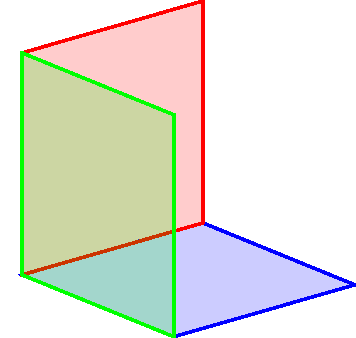
\includegraphics[width=\textwidth]{figures/3/manifold_a.pdf}
	\caption{Three perpendicular walls.}
	\label{fig:manifold_a}
\end{subfigure} \hfill%
\begin{subfigure}{0.45\textwidth}
	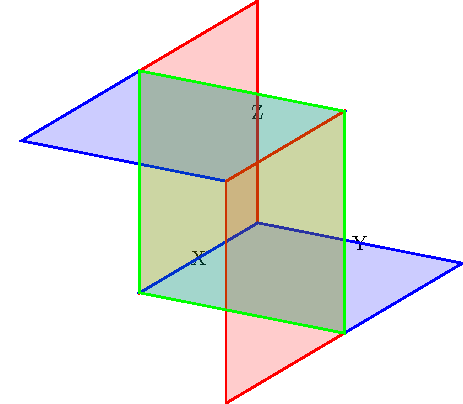
\includegraphics[width=\textwidth]{figures/3/manifold_b.pdf}
	\caption{Five perpendicular walls.}
	\label{fig:manifold_b}
\end{subfigure}
\caption{Two types of manifold used in our constructions.}
\label{fig:manifold_types}
\end{figure} 

%The set $M$, obtained from the union of mutually orthogonal faces of $G$, 
It bears mention that many lethal sets on manifolds are discovered through trial and error. One strategy is to imagine these manifolds as folded pieces of paper, and to identify lethal sets on their unfolded nets. This technique is discussed in more detail in Chapter \{CONSTRUCTIONS\}. 

\end{comment}


\chapter{A Tight Bound on Grids of Size $\geq$ 5}

Recall from Definition \ref{defn:thickness} that $G(a_1,a_2,a_3)$ represents the $[a_1] \times [a_2] \times [a_3]$ grid $G$, and that $\min\{a_1,a_2,a_3\}$ is the thickness of $G$. For example, the tuple $G(5,3,3)$ represents the thickness 3 grid $[5] \times [3] \times [3]$. In the following lemmas, we use the notation $(a_1,a_2,a_3)+(x_1,x_2,x_3) = (a_1+x_1, a_2+x_2, a_3+x_3)$ to represent an instance of Corollary \ref{cor:recursion} on the $3 \times 2$ matrix $A$:
$$A =
\begin{bmatrix}
a_1 & x_1 \\
a_2 & x_2 \\
a_3 & x_3
\end{bmatrix}.
$$
For example, the expression $(5,3,3) + (3,3,3)$ indicates an application of Corollary \ref{cor:recursion}, using the matrix $A = \begin{bsmallmatrix} 5&3&3 \\ 3&3&3 \end{bsmallmatrix}^T$, to obtain the tuple $(8,6,6)$. 

We shall call a thickness \emph{complete} if it can be shown that all divisibility cases in that thickness admit perfect lethal sets. In this section, we demonstrate that thickness 5, thickness 6 and thickness 7 are all complete. As these belong to the residue classes 2, 0, and 1 modulo 3, respectively, we then use Lemma \ref{lem:plus_333} to show that all larger grids are also complete. 

\section{Completeness of Thickness 5}
We show that all divisibility cases for grids of thickness 5 admit perfect lethal sets. Observe that divisibility cases for thickness 5 consist of grids $G(x,y,5)$ where $x$ and $y$ are in residue classes $\{0,2,3,5\}$ modulo 6 (see Table \ref{fig:thickness_5_cases}). We separate these divisibility cases into the following four categories and show that each category is complete:

\begin{enumerate}
\item $G(x,5,5)$ for $x \in \{2,5\} \pmod 6$ and $x \geq 5$;
\item $G(x,6,5)$ for $x \in \{0,3\} \pmod 6$ and $x \geq 5$;
\item $G(x,y,5)$ for $x,y \in \{0,2,3,5\} \pmod 6$, $x \not\equiv y \pmod 6$ and $x \geq 5$;
\item $G(x,y,5)$ for $x,y \in \{0,2,3,5\} \pmod 6$, $x \equiv y \pmod 6$ and $x \geq 5$;
\end{enumerate}

\begin{table}[]
\centering
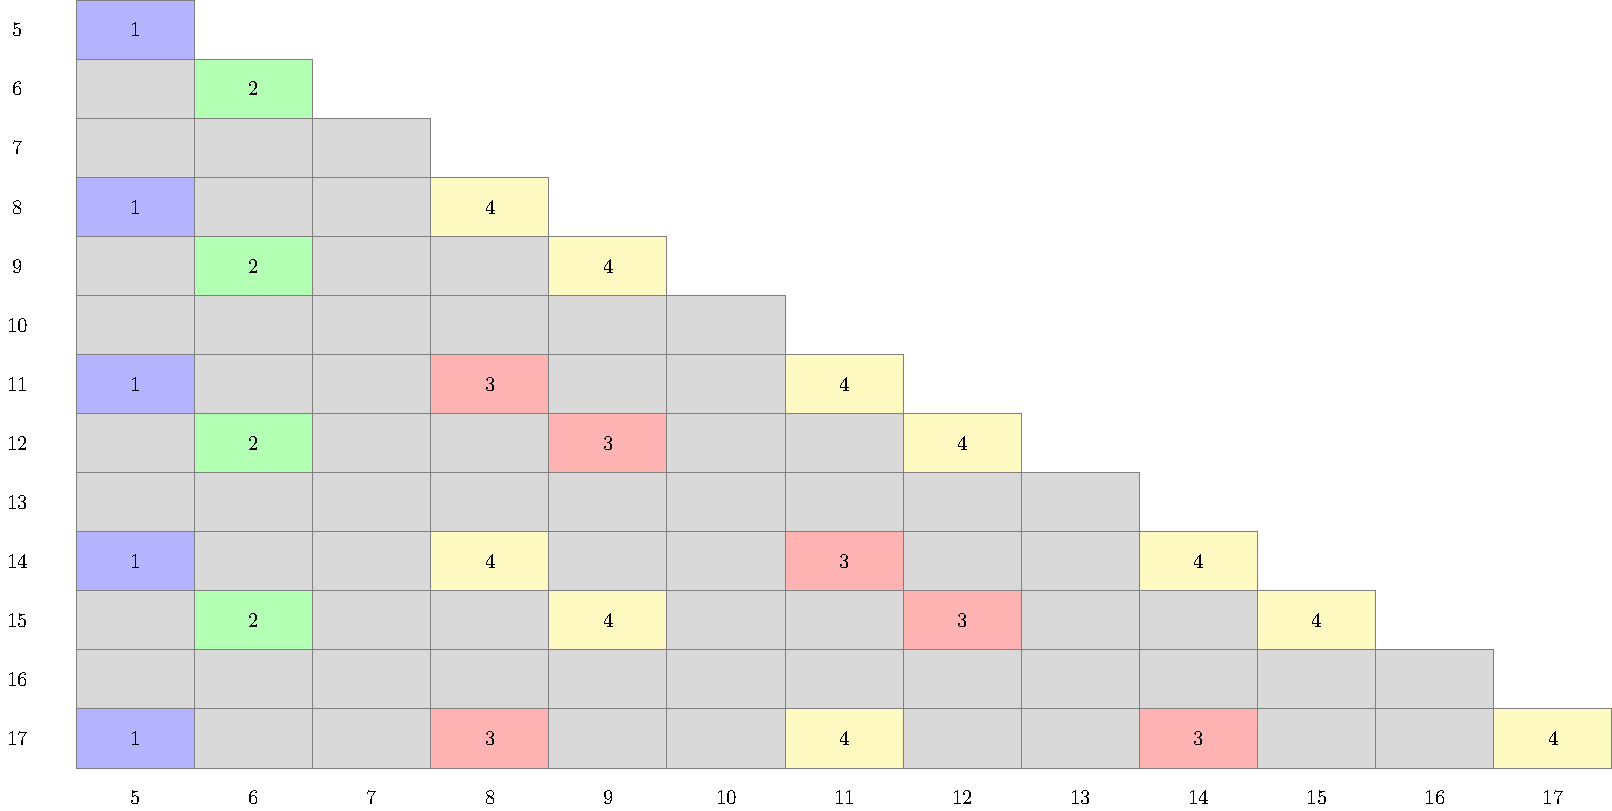
\includegraphics[width=\textwidth]{tables/4/thickness_5_cases.pdf}
\caption{The four thickness 6 cases analyzed in Lemmas \ref{lem:thickness_5_case_1} (blue), \ref{lem:thickness_5_case_2} (green), \ref{lem:thickness_5_case_3} (red), and \ref{lem:thickness_5_case_4} (yellow).}
\label{fig:thickness_5_cases}
\end{table}

%Leveraging \{lemmas from earlier chapters yet to be written\}, we show that all divisibility cases in thickness 5 percolate at the lower bound. 

%NOTE: THE FOLLOWING LEMMAS HOLD ASSUMING WE HAVE A GENERAL CONSTRUCTION FOR $(2,3,3k)$ FOR ALL $k$.
\begin{lem}
\label{lem:thickness_5_case_1}
All grids $G(x,5,5)$ for $x \in \{2,5\} \pmod 6$ and $x \geq 5$ admit perfect lethal sets.
\end{lem}

\begin{proof}
Consider $(5,2,2) + (a,3,3)$, for $a \equiv 0 \pmod 3$ and $a >3$. Observe that $(5+a,5,5)$ obtains all grids of the form described in Case 1, apart from $G(5,5,5)$ and $G(8,5,5)$.

By Corollary \ref{cor:recursion}, it suffices to show that $(5,2,2), (5,3,3), (a,2,3), (a,3,2)$ are all perfect. We have that $(5,2,2)$ is perfect by Construction \ref{con:5x2x2} in Appendix A, and $(5,3,3)$ is given by Proposition \ref{prop:3x3xk}. Since $a >3$, Propositions \ref{prop:2x3xk_0} and \ref{prop:2x3xk_3} give $(a,2,3)$. 

By Theorem \ref{thm:hypercubes} and Construction \ref{con:8x5x5} in Appendix A, we obtain the remaining grids $(5,5,5)$ and $(8,5,5)$, respectively. We conclude that all grids in Case 1 admit perfect lethal sets.
\end{proof}

\begin{lem}
\label{lem:thickness_5_case_2}
All grids $G(x,6,5)$ for $x \in \{0,3\} \pmod 6$ and $x \geq 5$ admit perfect lethal sets.
\end{lem}

\begin{proof}
Consider $(6,3,2) + (a,3,3)$, for $a \equiv 0 \pmod 3$ and $a >3$. Observe that $(6+a,6,5)$ obtains all grids of the form described in Case 2, apart from $G(6,6,5)$ and $G(9,6,5)$.

By Corollary \ref{cor:recursion}, we must show that $(6,3,2), (6,3,3), (a,3,3), (a,3,2)$ are all perfect. Since $a >3$, $(6,3,2)$ and $(a,3,2)$ are given by Propositions \ref{prop:2x3xk_0} and \ref{prop:2x3xk_3}. Similarly, $(6,3,3)$ and $(a,3,3)$ are given by Proposition \ref{prop:3x3xk}.

To obtain $(6,6,5)$, we consider $(3,3,1)+(3,3,4)$. By Corollary \ref{cor:recursion}, we must show that $(3,3,1), (3,3,4), (3,3,4), (3,3,1)$ are all perfect. These are obtained, respectively, by Propositions \ref{prop:3x3xk} and \ref{prop:thickness_3_width_4}. Construction \ref{con:9x6x5} gives $(9,6,5)$. We conclude that all grids in Case 2 admit perfect lethal sets.
\end{proof}

\begin{lem}
\label{lem:thickness_5_case_3}
All grids $G(x,y,5)$ for $x,y \in \{0,2,3,5\} \pmod 6$, $x \not\equiv y \pmod 6$, and $x,y \geq 5$ admit perfect lethal sets.
\end{lem}

\begin{proof}
Consider $(a,b,2) + (6,6,3)$, for $a,b \in \{0,2,3,5\} \pmod 6$, $a \not\equiv b \pmod 6$, and $a,b > 2$. Observe that $(a+6,b+6,5)$ obtains all grids of the form described in Case 3, apart from $G(a,8,5)$ for $a \equiv 5 \pmod 6$ and $a \geq 11$.

By Corollary \ref{cor:recursion}, we must show that $(a,b,2), (a,6,3), (6,b,3), (6,6,2)$ are all perfect. By Proposition \ref{prop:thickness_2_2d_family}, $(a,b,2)$ is perfect. Both $(a,6,3)$ and $(6,b,3)$ follow from Proposition \ref{prop:3x6xk}. We obtain $(6,6,2)$ from $(3,3,1)+(3,3,1)$. By Proposition \ref{prop:purina}, $(3,3,1)$ is perfect, and so by Corollary \ref{cor:recursion}, $(6,6,2)$ is perfect.

To obtain $(a,8,5)$, for $a \equiv 5 \pmod 6$ and $a \geq 17$, we consider $(8,5,2) + (a,3,3)$, for $a \equiv 3 \pmod 6$ and $a>3$. By Corollary \ref{cor:recursion}, we must show that $(2,5,2)$, $(8,3,3)$, $(a,5,3)$, $(a,2,3)$ are all perfect. We obtain $(2,5,2)$ from Construction \ref{con:5x2x2} and $(8,3,3)$ from Proposition \ref{prop:3x3xk}. Since $a \equiv 3 \pmod 6$, Proposition \ref{prop:thickness_2_2d_family} gives $(a,5,3)$, and Proposition \ref{prop:2x3xk_3} gives $(a,2,3)$. 

The above argument omits the singular grid $(11,8,5)$. However, we may obtain $(11,8,5)$ from $(2,3,6)+(3,5,5)$. By Corollary \ref{cor:recursion}, we must show that $(2,3,6), (2,5,5)$, $(3,3,5), (3,5,6)$ are all perfect. We obtain $(2,5,5)$ from Construction \ref{con:5x5x2}, $(3,3,5)$ from Proposition \ref{prop:3x3xk}, and $(2,3,6)$ and $(3,5,6)$ from Proposition \ref{prop:3x6xk}. We conclude that all grids in Case 3 admit perfect lethal sets.
\end{proof}

\begin{lem}
\label{lem:thickness_5_case_4}
All grids $G(x,y,5)$ for $x,y \in \{0,2,3,5\} \pmod 6$, $x \equiv y \pmod 6$, and $x \geq 5$ admit perfect lethal sets.
\end{lem}

\begin{proof}
Consider the construction $(a,b,2) + (6,3,3)$, for $a,b \in \{0,2,3,5\} \pmod 6$, $a \not\equiv b \pmod 6$, and $a,b > 2$. Observe that this construction obtains all grids of the form described in (4), apart from $(8,8,5)$.

By Corollary \ref{cor:recursion}, we must show that the grids $(a,b,2), (a,3,3), (6,b,3), (6,3,2)$ are all perfect. By Proposition \ref{prop:thickness_2_2d_family}, $(a,b,2)$ is perfect. Both $(6,3,2)$ and $(6,b,3)$ follow from Proposition \ref{prop:3x6xk}. We obtain $(a,3,3)$ from Proposition \ref{prop:3x3xk}.

To obtain $(8,8,5)$, we consider the construction $(2,2,2) + (6,6,3)$. By Corollary \ref{cor:recursion}, we must show that $(2,2,2), (2,6,6), (3,2,6), (3,6,2)$ are all perfect. We obtain $(2,2,2)$ from Theorem \ref{thm:hypercubes} and $(3,6,2)$ from Proposition \ref{prop:3x6xk}. The construction $(3,3,1)+(3,3,1)$ gives $(6,6,2)$. By Proposition \ref{prop:purina}, $(3,3,1)$ is perfect, and so by Corollary \ref{cor:recursion}, $(6,6,2)$ is perfect. We conclude that all grids of the form given in (3) admit perfect lethal sets.
\end{proof}

\begin{lem}
\label{lem:thickness_5_complete}
Thickness 5 is complete.
\end{lem}

\begin{proof}
By Lemmas \ref{lem:thickness_5_case_1}, \ref{lem:thickness_5_case_2}, \ref{lem:thickness_5_case_3}, and \ref{lem:thickness_5_case_4}, all divisibility cases for thickness 5 admit perfect lethal sets.
\end{proof}

\section{Completeness of Thickness 6}
We show that all divisibility cases for grids of thickness 6 admit perfect lethal sets. Observe that divisibility cases for thickness 6 consist of grids $G(x,y,6)$ where, without loss of generality, $x$ is in residue classes $\{0,3\}$ modulo 6, and $y$ is either even or odd (see Table \ref{fig:thickness_6_cases}). We separate these divisibility cases into the following four categories and show that each category is complete:

\begin{enumerate}
\item $G(x,y,6)$ for $x \equiv 0 \pmod 6$, $y \equiv 0 \pmod 2$, and $x,y \geq 6$;
\item $G(x,y,6)$ for $x \equiv 3 \pmod 6$, $y \equiv 1 \pmod 2$, and $x,y \geq 6$;
\item $G(x,y,6)$ for $x \equiv 3 \pmod 6$, $y \equiv 0 \pmod 2$, and $x,y \geq 6$;
\item $G(x,y,6)$ for $x \equiv 0 \pmod 6$, $y \equiv 1 \pmod 2$, and $x,y \geq 6$.
\end{enumerate}

%We shall show that all grids of thickness 6 can be obtained recursively from $(3n, m, 3)$, where $n,m \equiv 1 \pmod 2$ (this is that general thickness 3 construction), and one of $\{(3,3,3), (6,6,3), (6,3,3), (3,6,3)\}$. We examine each of these cases separately and show that each is complete. 

%(NOTE (to Peter and Jon): I have struggled a bit with the canonical way to describe grids. I like the tuple representation $(a,b,c)$ where WLOG $a \leq b \leq c$. However, this becomes a bit mucky in the following proofs, because $(3n,m,3)$ potentially violates this rule if $n$ is large and $m$ is small. To accommodate this, I have written ``grids of the form $(a,b,6)$, where $a \equiv 0 \pmod 6$ and $b \equiv 0 \pmod 2$, or $b \equiv 0 \pmod 6$ and $a \equiv 0 \pmod 2$," in an attempt to address the circumstance where the ordering of the tuple is flipped because $n$ is large and $m$ is small. However, I think this may just muddy the waters.)

%\begin{figure}[]
%\centering
%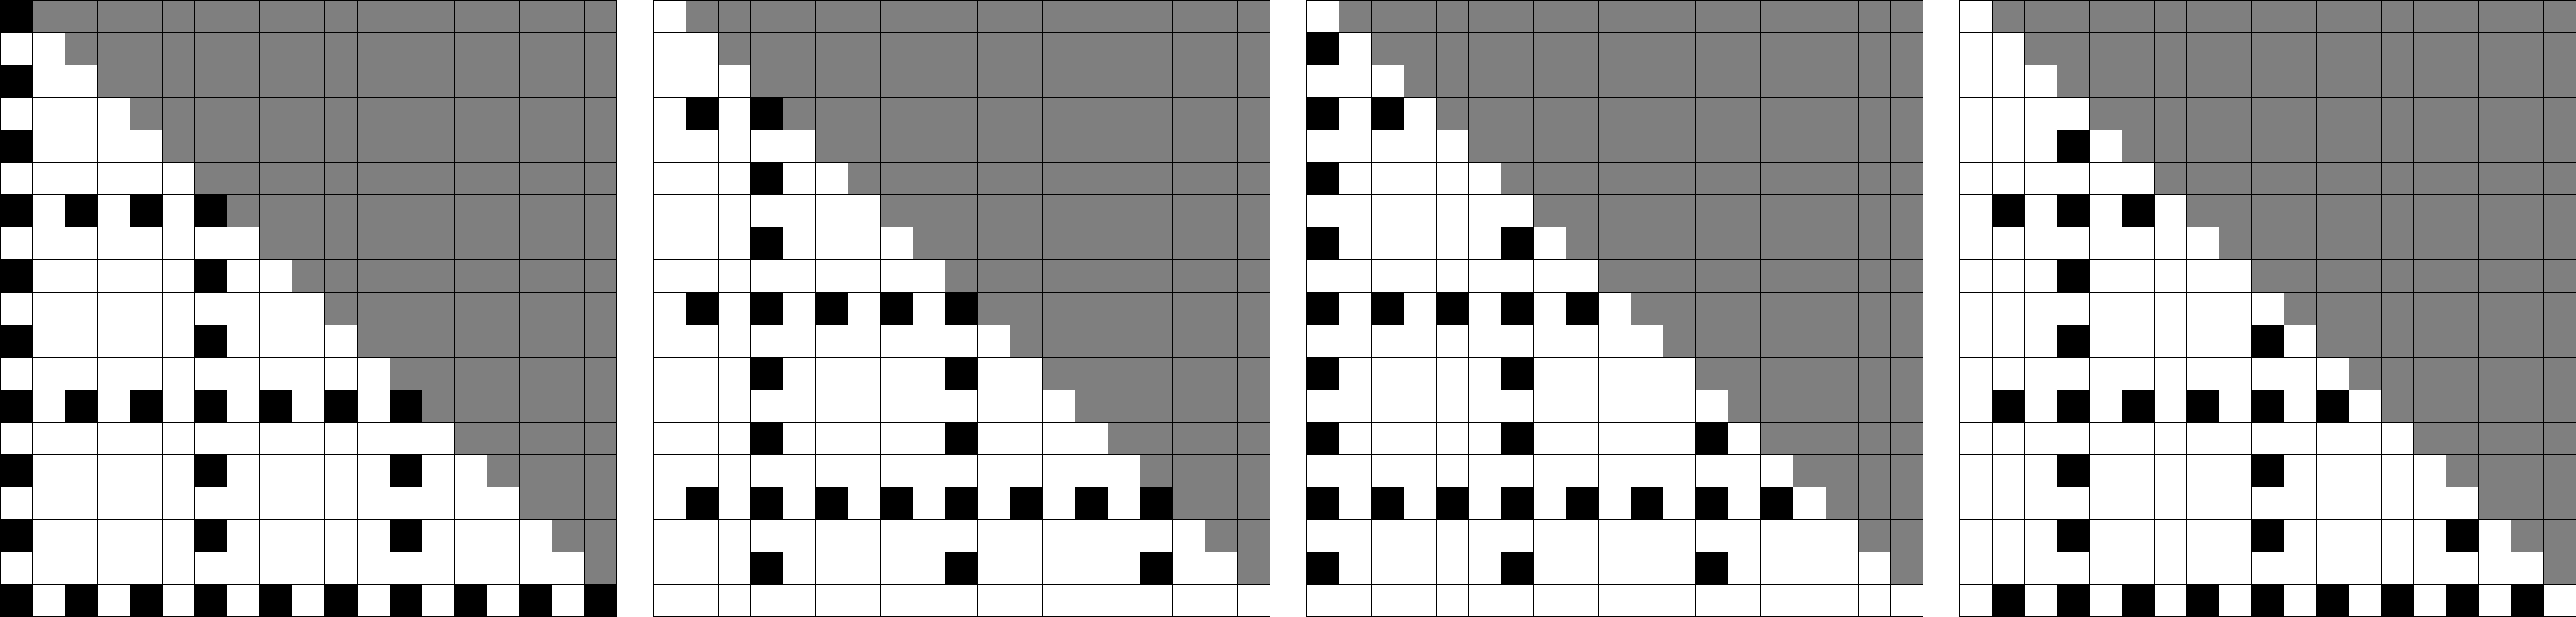
\includegraphics[width=\textwidth]{figures/4/thickness_6_case_1.pdf}
%\caption{Thickness 6 grids with perfect percolating sets as obtained in lemma \ref{lem:thickness_6_case_1} (left), and divisibility cases of thickness 6 (right).}
%\label{fig:thickness_6_case_1}
%\end{figure}

\begin{table}[]
\centering
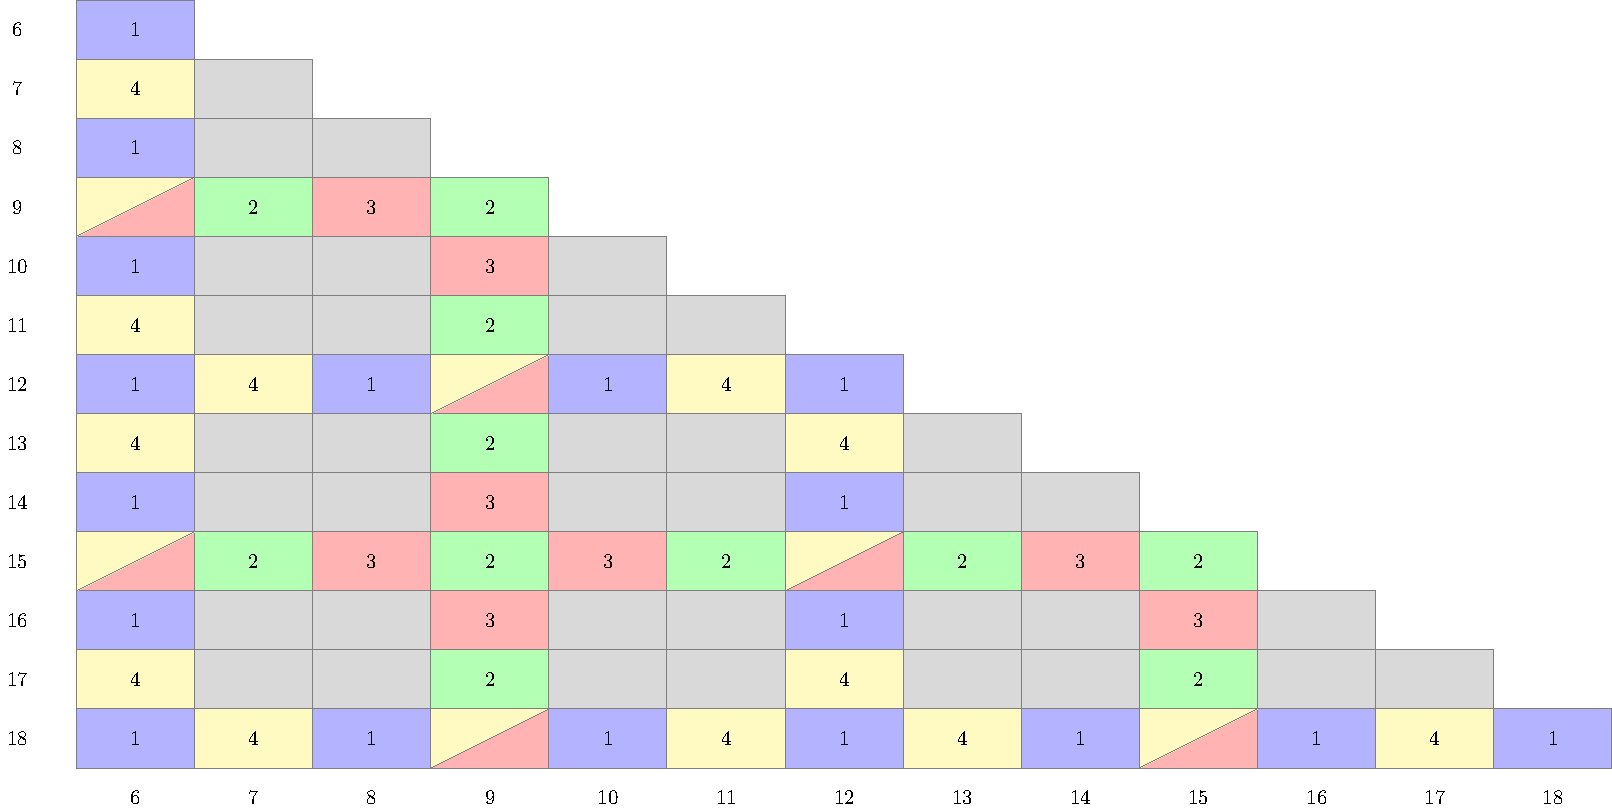
\includegraphics[width=\textwidth]{tables/4/thickness_6_cases.pdf}
\caption{The four thickness 6 cases analyzed in Lemmas \ref{lem:thickness_6_case_1} (blue), \ref{lem:thickness_6_case_2} (green), \ref{lem:thickness_6_case_3} (red), and \ref{lem:thickness_6_case_4} (yellow).}
\label{fig:thickness_6_cases}
\end{table}

\begin{lem}
\label{lem:thickness_6_case_1}
All grids $G(x,y,6)$ for $x \equiv 0 \pmod 6$, $y \equiv 0 \pmod 2$, and $x,y \geq 6$ admit perfect lethal sets.
\end{lem}

\begin{proof}
Consider $(3n,m,3) + (3,3,3)$, for $n,m \equiv 1 \pmod 2$ and $m > 1$. Observe that $(3n+3, m+3,6)$ obtains all grids of the form described in Case 1.

By Corollary \ref{cor:recursion}, we must show that $(3n,m,3), (3n,3,3), (3,m,3),(3,3,3)$ are all perfect. By Proposition \ref{prop:thickness_3_2d_family}, $(3n,m,3)$ is perfect for all $m > 1$. Since $n,m \neq 2$, $(3n,3,3), (3,m,3),(3,3,3)$ are all perfect by Proposition \ref{prop:3x3xk}. We conclude that all grids in Case 1 admit perfect lethal sets.
\end{proof}

\begin{lem}
\label{lem:thickness_6_case_2}
All grids $G(x,y,6)$ for $x \equiv 3 \pmod 6$, $y \equiv 1 \pmod 2$, and $x,y \geq 6$ admit perfect lethal sets.
\end{lem}

\begin{proof}
Consider $(3n,m,3) + (6,6,3)$, for $n,m \equiv 1 \pmod 2$ and $m > 1$. Observe that $(3n+6,m+6,6)$ obtains all grids of the form described in Case 2, apart from $G(x,7,6)$, for $x \equiv 3 \pmod 6$ and $x \geq 9$. 

By Corollary \ref{cor:recursion}, we must show that $(3n,m,3), (3n,6,3), (6,m,3), (6,6,3)$ are all perfect. By Proposition \ref{prop:thickness_3_2d_family}, $(3n,m,3)$ is perfect for all $m > 1$. Since $n,m > 1$, $(3n,6,3), (6,m,3), (6,6,3)$ are all perfect by Proposition \ref{prop:3x6xk}.

To obtain $(x,7,6)$, for $x \equiv 3 \pmod 6$ and $x \geq 9$, we consider $(6,3,3) + (x-6, 4,3)$. By Corollary \ref{cor:recursion}, we must show that $(6,3,3), (6,4,3), (x-6,3,3), (x-6,4,3)$ are all perfect. We obtain $(6,3,3)$ and $(x-6,3,3)$ from Proposition \ref{prop:3x6xk}. Proposition \ref{prop:3x6xk} gives $(6,4,3)$. Proposition \ref{prop:thickness_3_width_4} gives $(x-6,4,3)$. We conclude that all grids in Case 2 admit perfect lethal sets. 
\end{proof}

\begin{lem}
\label{lem:thickness_6_case_3}
All grids $G(x,y,6)$ for $x \equiv 3 \pmod 6$, $y \equiv 0 \pmod 2$, and $x,y \geq 6$ admit perfect lethal sets.
\end{lem}

\begin{proof}
Consider $(3n,m,3) + (6,3,3)$, for $n,m \equiv 1 \pmod 2$ and $m > 1$. Observe that $(3n+6,m+3,6)$ obtains all grids of the form described in Case 3. 

By Corollary \ref{cor:recursion}, we must show that $(3n,m,3), (3n,3,3), (6,m,3), (6,3,3)$ are all perfect. By Proposition \ref{prop:thickness_3_2d_family}, $(3n,m,3)$ is perfect for all $m > 1$. Since $m \neq 2$, $(6,m,3),(6,3,3)$ are both perfect by Proposition \ref{prop:3x3xk}. We obtain $(3n,3,3)$ by Proposition \ref{prop:3x3xk}. We conclude that all grids in Case 3 admit perfect lethal sets.
\end{proof}

\begin{lem}
\label{lem:thickness_6_case_4}
All grids $G(x,y,6)$, where $x \equiv 0 \pmod 6$, $y \equiv 1 \pmod 2$, and $x,y \geq 6$ admit perfect lethal sets.
\end{lem}

\begin{proof}
Consider $(3n,m,3) + (3,6,3)$, for $n,m \equiv 1 \pmod 2$ and $m > 1$. Observe that $(3n+3,m+6,6)$ obtains all grids described in Case 3, apart from $G(x,7,6)$, for $x \equiv 0 \pmod 6$ and $x \geq 6$. 

By Corollary \ref{cor:recursion}, we must show that $(3n,m,3)$, $(3n,6,3)$, $(3,m,3), (3,6,3)$ are all perfect. By Proposition \ref{prop:thickness_3_2d_family}, $(3n,m,3)$ is perfect for all $m > 1$. Since $n,m > 1$, $(3n,6,3)$ and $(3,6,3)$ are both perfect by Proposition \ref{prop:3x6xk}. Similarly, $(3,m,3)$ is perfect by Proposition \ref{prop:3x3xk}.

To obtain $(x,7,6)$, for $x \equiv 0 \pmod 6$ and $x \geq 6$, we consider $(3,3,3) + (x-3, 4,3)$. By Corollary \ref{cor:recursion}, we must show that $(3,3,3), (3,4,3), (x-3,3,3), (x-3,4,3)$ are all perfect. We obtain $(3,3,3), (3,4,3)$ and $(x-3,3,3)$ from Proposition \ref{prop:3x3xk}. Since $x \equiv 0 \pmod 6$, Proposition \ref{prop:thickness_3_width_4} gives $(x-6,4,3)$. We conclude that all grids given in Case 4 admit perfect lethal sets. 
\end{proof}

\begin{lem}
\label{lem:thickness_6_complete}
Thickness 6 is complete.
\end{lem}

\begin{proof}
All divisibility cases for thickness 6 are grids $G(x,y,6)$ such that at least one of $\{x,y\}$ is congruent to 0 modulo 3. Lemmas \ref{lem:thickness_6_case_1}, \ref{lem:thickness_6_case_2}, \ref{lem:thickness_6_case_3}, and \ref{lem:thickness_6_case_4} cover all such cases. The result follows.
\end{proof}

\section{Completeness of Thickness 7}

We show that all divisibility cases for grids of thickness 7 admit perfect lethal sets. Observe that divisibility cases for thickness 7 consist of grids $G(x,y,7)$ for $x,y$ in residue classes $\{0,1,3,4\}$ modulo 6 (see Table \ref{fig:thickness_7_cases}). We separate these divisibility cases into the following four categories and show that each category is complete:
\begin{enumerate}
\item $G(x,y,7)$ for $x,y \in \{1,4\}$, $x \equiv y \pmod 6$, and $x,y \geq 7$;
\item $G(x,y,7)$ for $x,y \in \{1,4\}$, $x \not\equiv y \pmod 6$, and $x,y \geq 7$;
\item $G(x,y,7)$ for $x,y \in \{0,3\}$, $x \equiv y \pmod 6$, and $x,y \geq 7$;
\item $G(x,y,7)$ for $x,y \in \{0,3\}$, $x \not\equiv y \pmod 6$, and $x,y \geq 7$.
\end{enumerate}

\begin{table}[]
\centering
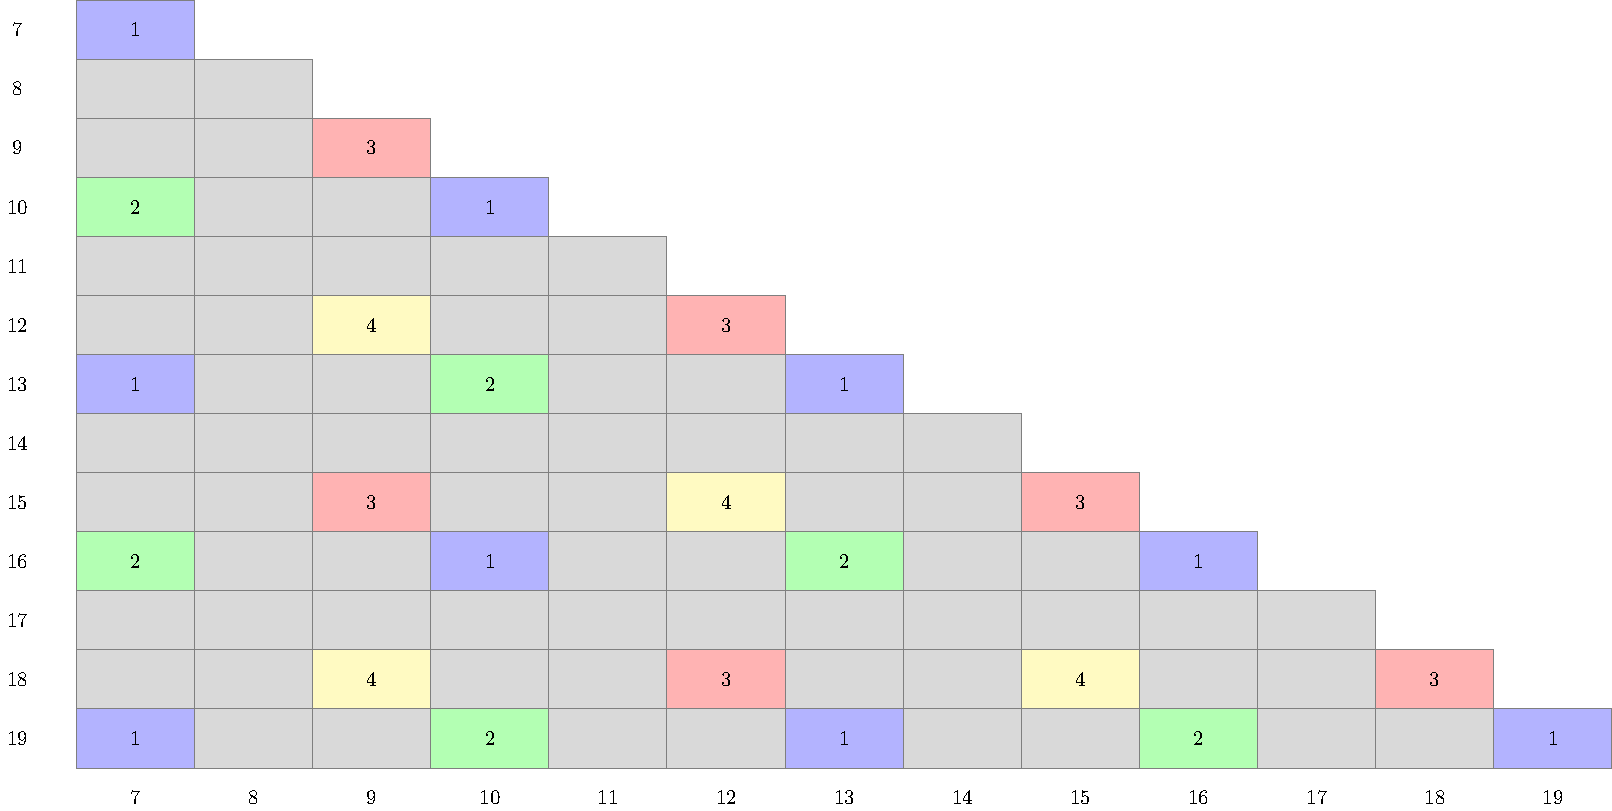
\includegraphics[width=\textwidth]{tables/4/thickness_7_cases.pdf}
\caption{The four thickness 7 cases analyzed in Lemmas \ref{lem:thickness_7_case_1} (blue), \ref{lem:thickness_7_case_2} (green), \ref{lem:thickness_7_case_3} (red), and \ref{lem:thickness_7_case_4} (yellow).}
\label{fig:thickness_7_cases}
\end{table}

\begin{lem}
\label{lem:thickness_7_case_1}
All grids $G(x,y,7)$ for $x,y \in \{1,4\}$, $x \equiv y \pmod 6$, and $x,y \geq 7$ admit perfect lethal sets.
\end{lem}

\begin{proof}
Consider $(a,b,2) + (8,5,5)$ for $a,b \in \{2,5\} \pmod 6$, $a \not\equiv b \pmod 6$, and $a,b > 2$. Observe that $(a+8,b+5,7)$ obtains all grids described in Case 1 above, apart from $G(10,10,7)$ and $G(a, 7,7)$, for $a \equiv 1 \pmod 6$. 

By Corollary \ref{cor:recursion}, we must show that $(a,b,2), (a,5,5), (8,b,5), (8,5,2)$ are all perfect. By Proposition \ref{prop:thickness_2_2d_family}, $(a,b,2)$ and $(8,5,2)$ are perfect. By Lemma \ref{lem:thickness_5_complete}, $(a,5,5)$ and $(8,b,5)$ are perfect. 

To obtain $(a,7,7)$, for $a \equiv 1 \pmod 6$, we consider $(4,4,4) + (a-4,3,3)$. By Corollary \ref{cor:recursion}, we must show that $(4,4,4), (4,3,3), (a-4,4,3), (a-4,3,4)$ are all perfect. We obtain $(4,4,4)$ from $(2,2,2)+(2,2,2)$. By Theorem \ref{thm:hypercubes} in Appendix A, we have that $(2,2,2)$ is perfect. Proposition \ref{prop:3x3xk} gives $(4,3,3)$. Since $a-4 \equiv 3 \pmod 6$, we obtain $(a-4,4,3)$ from Proposition \ref{prop:thickness_3_width_4}.

To obtain $(10,10,7)$, consider $(5,5,5) + (5,5,2)$. By Corollary \ref{cor:recursion}, we must show that $(5,5,5), (5,5,2), (5,5,2), (5,5,5)$ are all perfect. Lemma \ref{lem:thickness_5_complete} gives us $(5,5,5)$, and Construction \ref{con:5x5x2} gives us $(5,5,2)$. We conclude that all grids in Case 1 admit perfect lethal sets. 
\end{proof}

\begin{lem}
\label{lem:thickness_7_case_2}
All grids $G(x,y,7)$ for $x,y \in \{1,4\}$, $x \not\equiv y \pmod 6$, and $x,y \geq 7$ are complete.
\end{lem}

\begin{proof}
Consider $(a,b,2) + (5,5,5)$ for $a,b \in \{2,5\} \pmod 6$, $a \not\equiv b \pmod 6$, and $a,b > 2$. Observe that $(a+5,b+5,7)$ obtains all grids described in Case 2 above, apart from $G(a,7,7)$, for $a \equiv 4 \pmod 6$. 

By Corollary \ref{cor:recursion}, we must show that $(a,b,2), (a,5,5), (5,b,5), (5,5,2)$ are all perfect. By Proposition \ref{prop:thickness_2_2d_family}, $(a,b,2)$ is perfect. We obtain $(a,5,5)$ and $(5,b,5)$ from Lemma \ref{lem:thickness_5_complete}, and $(5,5,2)$ is given by Construction \ref{con:5x5x2}.

To obtain $(a,7,7)$, for $a \equiv 4 \pmod 6$, we consider $(7,4,4) + (a-7,3,3)$. Since $a \equiv 4 \pmod 6$ and $a \geq 7$, we have that $a \geq 10$. By Corollary \ref{cor:recursion}, we must show that $(7,4,4), (7,3,3), (a-7,4,3), (a-7,3,4)$ are all perfect. We obtain $(7,4,4)$ from $(2,2,2) + (5,2,2)$. Theorem \ref{thm:hypercubes} and Construction \ref{con:5x2x2} show that $(2,2,2)$, $(2,2,2)$, $(5,2,2)$, $(5,2,2)$ are all perfect. Proposition \ref{prop:3x3xk} gives us $(7,3,3)$. Since $a-7 \equiv 3 \pmod 6$, we obtain $(a-7,4,3)$ from Proposition \ref{prop:thickness_3_width_4}. We conclude that all grids in Case 2 admit perfect lethal sets. 
\end{proof}

\begin{lem}
\label{lem:thickness_7_case_3}
All grids $G(x,y,7)$ for $x,y \in \{0,3\}$, $x \equiv y \pmod 6$, and $x,y \geq 7$ are complete.
\end{lem}

\begin{proof}
Consider $(a,b,2) + (6,9,5)$ for $a,b \in \{0,3\} \pmod 6$, $a \not\equiv b \pmod 6$, and $a,b > 2$. Observe that $(a+6,b+9,7)$ contains all grids described in Case 3 above, apart from $G(9,9,7)$. 

By Corollary \ref{cor:recursion}, we must show that $(a,b,2), (a,9,5), (6,b,5), (6,9,2)$ are all perfect. By Proposition \ref{prop:thickness_2_2d_family}, $(a,b,2)$ and $(6,9,2)$ are perfect. By Proposition \ref{prop:thickness_3_2d_family}, $(a,9,5)$ is perfect. We obtain $(6,b,5)$ from Lemma \ref{lem:thickness_5_complete}, for $b \geq 5$, and $(6,3,5)$ from Proposition \ref{prop:3x6xk}. 

To obtain $(9,9,7)$, consider $(6,6,4) + (3,3,3)$. By Corollary \ref{cor:recursion}, we must show that $(6,6,4), (6,3,3), (3,6,3), (3,3,4)$ are all perfect. We obtain $(6,6,4)$ from $(3,3,1) + (3,3,3)$. Construction \ref{con:3x3x1} shows that $(3,3,1)$ is perfect. Proposition \ref{prop:3x3xk} gives us $(6,3,3)$, $(3,3,3)$ and $(4,3,3)$. We conclude that all grids in Case 3 admit perfect lethal sets.
\end{proof}

\begin{lem}
\label{lem:thickness_7_case_4}
All grids $G(x,y,7)$ for $x,y \in \{0,3\}$, $x \not\equiv y \pmod 6$, and $x,y \geq 7$ are complete.
\end{lem}

\begin{proof}
Consider $(a,b,2) + (6,6,5)$ for $a,b \in \{0,3\} \pmod 6$, $a \not\equiv b \pmod 6$, and $a,b > 2$. Observe that $(a+6,b+6,7)$ contains all grids described in Case 4 above. 

By Corollary \ref{cor:recursion}, we must show that $(a,b,2), (a,6,5), (6,b,5), (6,6,2)$ are all perfect. By Proposition \ref{prop:thickness_2_2d_family}, $(a,b,2)$ is perfect. We obtain $(6,b,5)$ from Lemma \ref{lem:thickness_5_complete}, for $b \geq 5$, and $(6,3,5)$ from Proposition \ref{prop:3x6xk}. We obtain $(6,6,2)$ from $(3,3,1)+(3,3,1)$. By Proposition \ref{prop:purina}, $(3,3,1)$ is perfect, and so by Corollary \ref{cor:recursion}, $(6,6,2)$ is perfect. We conclude that all grids in Case 4 admit perfect lethal sets.
\end{proof}

\begin{lem}
Thickness 7 is complete.
\end{lem}

\begin{proof}
\label{lem:thickness_7_complete}
By Lemmas \ref{lem:thickness_7_case_1}, \ref{lem:thickness_7_case_2}, \ref{lem:thickness_7_case_3}, and \ref{lem:thickness_7_case_4}, all divisibility cases for thickness 7 admit perfect lethal sets.
\end{proof}

\section{Proof of the Main Result}

We are now in a position to prove Theorem \ref{thm:main_result}. We first state the following auxiliary result for divisibility cases. 

\begin{cor}
\label{cor:divisibility_complete}
Let $G(a_1,a_2,a_3)$ be a divisibility case, for $a_1, a_2, a_3 \geq 5$. Then $G(a_1,a_2,a_3)$ admits a perfect lethal set.
\end{cor}

\begin{proof}
By Lemmas \ref{lem:thickness_5_complete}, \ref{lem:thickness_6_complete}, and \ref{lem:thickness_7_complete}, all divisibility cases for $G(a_1,a_2,5)$, $G(a_1,a_2,6)$, and $G(a_1,a_2,7)$ admit perfect lethal sets. Observe that $(a_1,a_2,a_3) + (3,3,3)$ gives a one-to-one mapping from divisible grids of thickness $a_3$ to divisible grids of thickness $a_3+3$. By Lemma \ref{lem:plus_333}, if $(a_1,a_2,a_3)$ is perfect, then $(a_1,a_2,a_3) + (3,3,3)$ is perfect. Therefore, since each residue class modulo 3 is complete, all divisibility cases $G(a_1,a_2,a_3)$, for $a_1, a_2, a_3 \geq 5$, admit perfect lethal sets.
\end{proof}

The proof of Theorem \ref{thm:main_result} requires further implementation of the recursive process outlined in Lemma \ref{lem:recursion}. In particular, we leverage Corollary \ref{cor:divisibility_complete} to prove the following helpful lemma:

%\begin{lem}
%Let $(a_1,a_2,a_3)$ be any grid such that $a_1 \geq a_2 \geq a_3 \geq 5$. Let $b_1, b_2, b_3$ be integers such that $b_1 \equiv b_2 \equiv b_3 \equiv 0 \pmod 3$ and $b_1, b_2, b_3 \geq 6$. Suppose $(a_1,a_2,a_3)$ admits an optimal lethal set. Then $(a_1,a_2,a_3) + (b_1,b_2,b_3)$ is optimal.
%\end{lem}

%\begin{proof}
%By Corollary \ref{cor:recursion}, we must show that $(a_1,b_2,b_3), (b_1,a_2,b_3), (b_1,b_2,a_3)$ are all perfect. Since $b_1 \equiv b_2 \equiv b_3 \equiv 0 \pmod 3$, each of these grids is divisible. Furthermore, since $a_1,a_2,a_3,b_1, b_2, b_3 \geq 5$, by Corollary \ref{cor:divisibility_complete}, each grid is perfect.
%\end{proof}

\begin{lem}
\label{lem:multiples_of_3}
Let $G(a_1,a_2,a_3)$ be any grid such that $a_1, a_2, a_3 \geq 5$. If $(a_1,a_2,a_3)$ is optimal, then $(a_1,a_2,a_3) + (3b_1,3b_2,3b_3)$ is optimal for $b_1,b_2,b_3 \geq 2$. 
\end{lem}

\begin{proof}
By Corollary \ref{cor:recursion}, we must show that $(a_1,3b_2,3b_3), (3b_1,a_2,3b_3), (3b_1,3b_2,a_3)$ are all perfect. Since $3b_1 \equiv 3b_2 \equiv 3b_3 \equiv 0 \pmod 3$, each of these grids is divisible. Furthermore, each grid has minimum thickness 5 and so, by Corollary \ref{cor:divisibility_complete}, each grid is perfect.
\end{proof}

Let $(r_1,r_2,r_3)$ be the tuple of residues of $(a_1,a_2,a_3)$ modulo 3. Given an optimal grid $G(a_1,a_2,a_3)$, Lemma \ref{lem:multiples_of_3} says that all other grids of size at least $G(a_1+6,a_2+6,a_3+6)$ with the same $(r_1,r_2,r_3)$ are optimal. Therefore, by obtaining optimal lethal sets on the smallest grids for each residue tuple $(r_1,r_2,r_3)$, we are able to obtain a lower bound on the size of all optimal grids under 3-neighbor percolation (see Table \ref{tab:residues}).

\begin{table}[]
\centering
\begin{subfigure}{0.3\textwidth}
	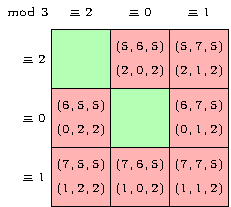
\includegraphics[width=\textwidth]{tables/4/residue_2.pdf}
	%\caption{Thickness 5}
	\label{tab:r_a}
\end{subfigure} \hfill%
\begin{subfigure}{0.3\textwidth}
	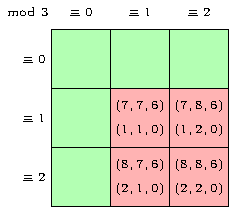
\includegraphics[width=\textwidth]{tables/4/residue_0.pdf}
	%\caption{Thickness 6}
	\label{tab:r_b}
\end{subfigure} \hfill%
\begin{subfigure}{0.3\textwidth}
	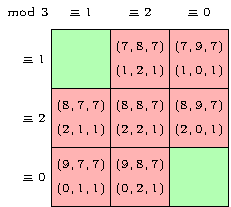
\includegraphics[width=\textwidth]{tables/4/residue_1.pdf}
	%\caption{Thickness 7}
	\label{tab:r_c}
\end{subfigure}
\caption{Residue tuples for non-divisibility cases in thicknesses 5, 6, and 7. Top tuple is grid dimension, bottom tuple is residues modulo 3.}
\label{tab:residues}
\end{table} 

\begin{proof}[Proof of Theorem \ref{thm:main_result}]
Let $(a_1,a_2,a_3)$ be such that $a_1, a_2, a_3 \geq 11$. Observe that each $a_i$ can be written as $3b_i + r_i$, for $b_i \geq 2$ and some $r_i \in \{5,6,7\}$. We therefore have that $(a_1,a_2,a_3) = (r_1,r_2,r_3) + (3b_1,3b_2,3b_3)$, for $r_1,r_2,r_3 \in \{5,6,7\}$. By Lemma \ref{lem:multiples_of_3}, $(a_1,a_2,a_3)$ is optimal if $(r_1,r_2,r_3)$ is optimal. 

Corollary \ref{cor:divisibility_complete} gives us the optimality of divisibility cases. Therefore, we need only consider non-divisible grids $G(r_1,r_2,r_3)$. In particular, we must show that $(6,5,5)$, $(7,5,5)$, $(7,6,5)$, $(7,7,5)$ and $(7,7,6)$ are all optimal. We obtain $(7,7,6)$ from $(4,4,3) + (3,3,3)$. By Lemma \ref{lem:plus_333}, $(7,7,6)$ is optimal. Constructions for $(6,5,5)$, $(7,5,5)$, $(7,6,5)$, $(7,7,5)$ are given in Appendix A.

Since each of the non-divisibility grids $G(r_1,r_2,r_3)$ admits an optimal lethal set, we conclude that all grids $G(a_1,a_2,a_3)$ where $a_1, a_2, a_3 \geq 11$ are optimal.
\end{proof}

%\begin{lem}
%Let $R$ be a minimum set of grids representing each unique non-divisible residue tuple modulo 3. Without loss of generality, suppose $a_1 \geq a_2 \geq a_3$ for all $(a_1,a_2,a_3) \in R$, and let $a$ be the minimum value of $a_3$. If each $G \in R$ admits an optimal lethal set, then all non-divisible grids $(a_1,a_2,a_3)$, where $a_1, a_2, a_3 \geq a+6$, are optimal.
%\end{lem}

% COMMENT
% COMMENT
% COMMENT
% COMMENT
% COMMENT

\begin{comment}

Let $(a,b,2)$ represent an arbitrary (divisible) grid of thickness 2, and let $x = a \pmod 6$ and $y = b \pmod 6$. By \{some as of yet unwritten construction\}, we have that $(a,b,2)$ percolates at the lower bound for all $x,y \in \{0,2,3,5\}$, where $x \neq y$. We consider two constructions: $(a,b,2) + (6,3,3)$ and $(a,b,2) + (6,6,3)$. 

By item (1) of the remark, in order to show that $(a,b,2) + (6,3,3)$ percolates at the lower bound, it is sufficient to show that $(a,b,2), (a,3,3), (6,b,3), (6,3,2)$ all percolate at the bound. By \{more unwritten constructions\}, this is true for all $x,y \in \{0,2,3,5\}$, where $x \neq y$, $a,b > 1$, and at least one of $\{a,b\} > 2$. (Note that if $a=2$, one of the tuples is $(2,3,3)$, which does not percolate at the lower bound; we accommodate for this by re-writing $(a,b,2) + (6,3,3)$ as $(a,b,2) + (3,6,3)$.) The resulting tuple $(a', b', 5)$ is a grid of thickness 5, with $a'$ and $b'$ in the same residue class modulo $6$, $x,y \geq 8$, and at least one of $\{a',b'\} \geq 9$. From \{some figure representing the divisibility cases of thickness 5\}, we see that the lower bound on $a'$ and $b'$ omits all grids of the form $(5,5,k)$ and $(5,6,k)$, as well as the singular grid $(8,8,5)$. 

Applying an analogous argument to $(a,b,2) + (6,6,3)$, we must demonstrate that $(a,b,2), (a,6,3), (6,b,3), (6,6,2)$ all percolate at the lower bound. By \{some other constructions\}, we again find that this holds for all $x,y \in \{0,2,3,5\}$, where $x \neq y$ and $a,b > 1$. This gives all thickness 5 tuples $(a',b', 5)$ with $a'$ and $b'$ in different residue classes modulo $6$, where $a',b' \geq 8$. 

Combining these results, we have completeness for all grids of thickness 5 except those of the form $(5,5,k)$ and $(5,6,k)$, and the singular grid $(8,8,5)$. By lemmas \ref{lem:width_5} and \ref{lem:width_6}, and \{some construction for $(8,8,5)$\}, these cases are also complete, and so thickness 5 is complete. This completes the proof. 

\end{comment}






%\chapter{Tight Bound on $(a,b,c)$ Grids for $a \geq b \geq c \geq 11$}


\chapter{Thickness One}

While results from the previous chapters resolve the question of $m(a_1,a_2,a_3,3)$ for $a_1 \geq a_2 \geq a_3 \geq 11$, similar constructions for smaller grids remain sparse. Nevertheless, computer examples seem to suggest that grids of minimum size at least 2 are largely optimal. Grids of thickness 1 tell a different story. In this chapter, we prove that the only perfect grids in thickness 1 are those of the form $[2^n-1]^2$. This answers a question posed by Benevides et al. in \cite{benevides}.

\section{A tight result for $[n]^2$}
The argumentative structure of the proof is as follows: Let $A_0$ be a perfect lethal set on the grid $(a_1, a_2, 1)$. We show that the structure of $A_0$ guarantees the existence of a perfect lethal set on the smaller grid $(\frac{a_1-1}{2}, \frac{a_2-1}{2}, 1)$. Repeated applications of this process of reduction guarantee the existence of a perfect lethal set on the grid $(a_0, 1,1)$. Since the only such grid that admits a perfect lethal set is $(1,1,1)$, we are forced to conclude that $a_1 = a_2 = 2^k-1$ for some $k > 0$. 

\subsection{Preliminaries}
For the remainder of the chapter, let $G = [a_1] \times [a_2]$. Recall that perfect lethal sets match the surface area bound. In particular,
$$|A_0| = \frac{a_1a_2 + a_1 + a_2}{3}.$$
We begin with the following observations regarding the structure of $A_0$:

\begin{prop}
\label{prop:alternating_border}
If $A_0$ is a perfect lethal set on $G$, then $A_0$ contains alternating vertices along the border of $G$. 
\end{prop}

\begin{proof}
Since $A_0$ is perfect, it must form an independent set in $G$. By Proposition \ref{prop:border}, no two adjacent border vertices are both uninfected. Together, these conditions ensure that $A_0$ intersects the border of $G$ in an alternating pattern (see Figure \ref{fig:border}). 
\end{proof}

\begin{figure}[]
\centering
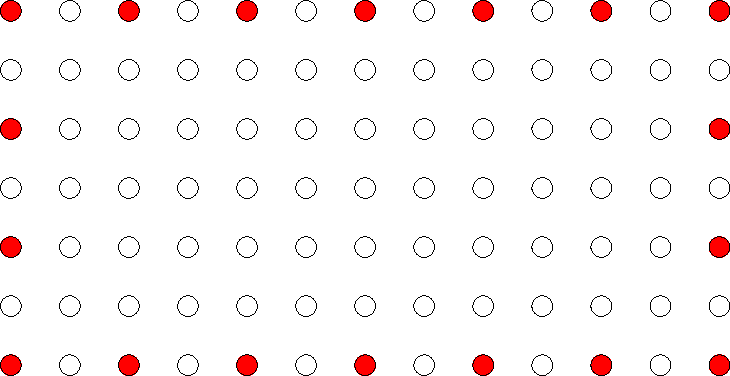
\includegraphics[width=0.5\textwidth]{figures/6/border.pdf}
\caption{Alternating infection along the border of $[7] \times [13]$.}
\label{fig:border}
\end{figure} 

\begin{prop}
\label{prop:odd_by_odd}
If $A_0$ is a perfect lethal set on $G$, then $a_1, a_2 \equiv 1 \pmod 2$.
\end{prop}

\begin{proof}
By Propositions \ref{prop:alternating_border} and \ref{prop:corners}, $a_1, a_2 \equiv 1 \pmod 2$.
\end{proof}

\begin{prop}
\label{prop:one_border_vertex}
Let $A_0$ be a perfect lethal set on $[a_1] \times [a_2]$ under 3-neighbor percolation. Let $H = V([a_1] \times [a_2]) \setminus A_0$. Then the subgraph induced by $H$ is acyclic and each component of $H$ contains exactly one border vertex.
\end{prop}

\begin{proof}
Sufficiency follows from Proposition \ref{prop:immune_regions}. For necessity, observe that the interior vertices of $A_0$ each remove exactly 4 edges from the subgraph induced by $H$. This implies that the subgraph induced by $H$ is a forest with exactly $a_1 + a_2 - 2$ components. As there are exactly $a_1 + a_2 - 2$ border vertices in $H$, each component must contain exactly one border vertex.
\end{proof}

Consider a labeling of the vertices of $G$ by their coordinates, starting at $(1,1)$ in the lower left and ranging to $(a_1,a_2)$ in the upper right. Refer to a vertex $(x,y)$ as ``even" or ``odd" depending on the parity of $x+y$. If a set $S \subseteq V(G)$ contains all vertices of the same parity, call $S$ monochromatic. The following lemma leverages the prior propositions to prove that any perfect lethal set on $G$ must be monochromatic.

\begin{lem}
Let $A_0$ be a perfect lethal set on $G$. Then $A_0$ is monochromatic with respect to the proper 2-coloring of $G$.
\end{lem}

\begin{proof}
From Proposition \ref{prop:alternating_border}, observe that $A_0$ contains all even vertices along the border of $G$. Suppose for contradiction that $A_0$ also contains odd vertices. We show that this implies the existence of a cycle in the subgraph induced by $V(G) \setminus A_0$, contradicting Proposition \ref{prop:one_border_vertex}. 

Let $H$ be a graph with vertices $V(H) = V(G)$ and edges $uv$ if and only if $u$ and $v$ are diagonally adjacent in $G$. Consider the subgraph of $H$ induced by the odd vertices of $A_0$ and let $K$ be a connected component. Observe that $K$ is acyclic: any cycle in $K$ encloses a component of $G[\overline{A_0}]$, contradicting Proposition \ref{prop:one_border_vertex}. Furthermore, by Proposition \ref{prop:alternating_border}, all vertices of $K$ are in the interior of $G$. Let $C_H$ be the cycle induced in $H$ by $N_G(K)$. Note that since $A_0$ is an independent set, $N_G(K) \cap A_0 = \emptyset$ and $C_H \cap A_0 = \emptyset$. Consider the closed walk induced in $G$ by the vertices $V(C_H) \cup N_H(K) \setminus A_0$. This walk describes a cycle $C_G$ in $G[\overline{A_0}]$, which contradicts Proposition \ref{prop:one_border_vertex}.
 \end{proof}

\begin{figure}[]
\centering
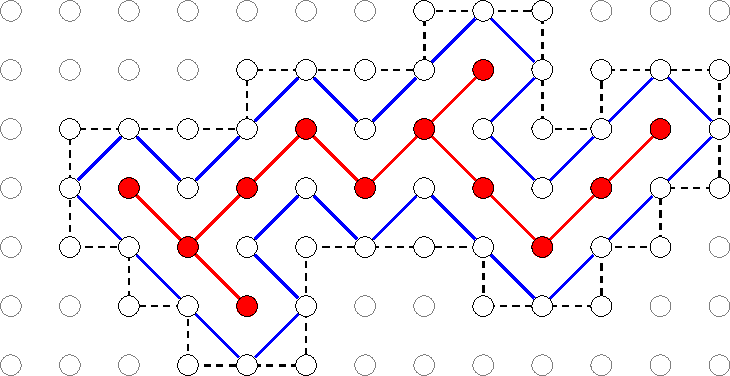
\includegraphics[width=0.5\textwidth]{figures/6/monochromatic.pdf}
\caption{$[7] \times [13]$ grid with component $K$ (red), $C_H$ (blue), and $C_G$ (dashed).}
\label{fig:border}
\end{figure} 

\subsection{Reduction}
We present an auxiliary $(\frac{a_1-1}{2}, \frac{a_2-1}{2}, 1)$ grid $G'$ obtained from $G$, and show that it admits a perfect lethal set. Let the vertices of $G'$ be $2 \times 2$ tiles of $G$ given by
$$\{(2x-1,2y-1),(2x-1,2y),(2x,2y-1),(2x,2y) \mid (x,y) \in [1, (a_1-1)/2] \times [1, (a_2-1)/2]\},$$
with adjacencies between tiles that differ by one in each of the cardinal directions. Note that Proposition \ref{prop:odd_by_odd} ensures that $|V(G')|$ is an integer. Furthermore, observe that for any tile $T_{x,y} \in V(G')$, $|A_0 \cap T_{x,y}| \in \{1,2\}$. This follows from the fact that $A_0$ is an independent set, and $G[\overline{A_0}]$ is acyclic. For all $T_{x,y} \in V(G')$, color $T_{x,y}$ blue if $|A_0 \cap T_{x,y}| = 2$, and white otherwise. Let $b$ and $w$ be the number of blue and white tiles in $V(G')$, respectively. We determine $b$ by solving the following system of equations:
\begin{align*}
b + w &= \frac{(a_1-1)(a_2-1)}{4} \\
2b + w &= \frac{a_1a_2+a_1+a_2}{3} - \frac{a_1+a_2}{2}.
\end{align*}
This gives the following expression for $b$:
\begin{align}
\frac{a_1a_2+a_1+a_2}{3} - \frac{a_1+a_2}{2} - \frac{(a_1-1)(a_2-1)}{4} &= \frac{a_1a_2+a_1+a_2-3}{12} \label{eq:tile_bound_1} \\
&= \frac{(\frac{a_1-1}{2})(\frac{a_2-1}{2}) + \frac{a_1-1}{2} + \frac{a_2-1}{2}}{3} \label{eq:tile_bound_2}.
\end{align}
Note that this is precisely the surface area bound for the $(\frac{a_1-1}{2}, \frac{a_2-1}{2}, 1)$ grid. Furthermore, since $a_1 \equiv a_2 \equiv 1 \pmod 6$ or $a_1 \equiv a_2 \equiv 3 \pmod 6$, all terms on the LHS of \ref{eq:tile_bound_1} are integral, and so the SA bound in \ref{eq:tile_bound_2} is tight.

\begin{figure}[]
\centering
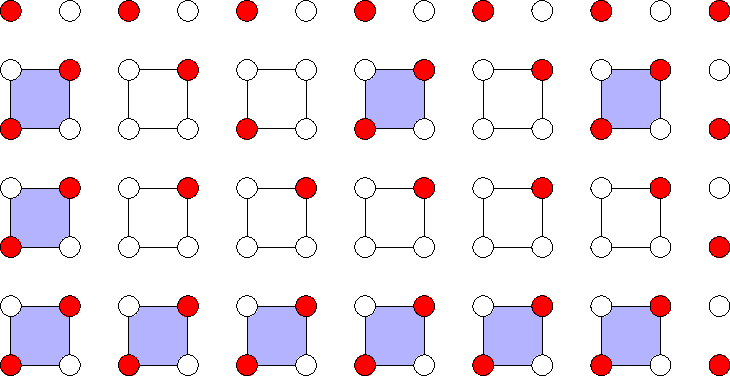
\includegraphics[width=0.5\textwidth]{figures/6/tiles.pdf}
\caption{$[7] \times [13]$ grid with $T_{x,y}$ colored blue if $|T_{x,y} \cap A_0| = 2$. Note that $A_0$ is \emph{not} perfect.}
\label{fig:tiles}
\end{figure} 

We prove that the blue tiles form a lethal set in $G'$. We begin with the following observation:

\begin{prop}
\label{prop:bottom_left}
All white tiles have their $A_0$-vertex in the bottom left corner.
\end{prop}

\begin{proof}
For contradiction, suppose that there exists a white tile $T_0$ with one infected vertex in the upper right. By Proposition \ref{prop:one_border_vertex}, there exists a path in $G[\overline{A_0}]$ from $T_0 \setminus A_0$ to the border. We consider the sequence of white tiles $T_0, \dots, T_n$ containing this path. 

Consider two consecutive tiles $T_i, T_{i+1}$ in this sequence. Note that $T_i$ and $T_{i+1}$ cannot be diagonally adjacent, as such a configuration creates a 4-cycle in $G[\overline{A_0}]$ (see Figure \ref{fig:tile_cycle}). Additionally, by Proposition \ref{prop:alternating_border}, observe that $T_n$ has its infected vertex in the bottom left corner. Therefore, since $T_0$ contains an infection in the top right by assumption, there exist tiles $T_i, T_{i+1}$ such that $T_i$ has an infection in the top right, and $T_{i+1}$ has an infection in the bottom left. 

We consider two cases. If $T_{i+1}$ is below or to the left of $T_i$, we obtain a 4-cycle. On the other hand, if $T_{i+1}$ is above or to the right of $T_i$, there is no path in $G[\overline{A_0}]$ between them (see Figure \ref{fig:tile_cases}). We therefore conclude that $T_0$ must have an infected vertex in the bottom left.
\end{proof}

\begin{figure}[]
\centering
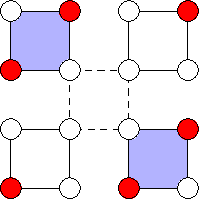
\includegraphics[width=0.15\textwidth]{figures/6/tile_cycle.pdf}
\caption{Diagonal white tiles and the resulting 4-cycle.}
\label{fig:tile_cycle}
\end{figure} 

\begin{figure}[]
\centering
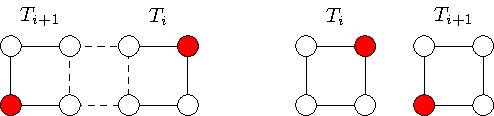
\includegraphics[width=0.5\textwidth]{figures/6/tile_cases.pdf}
\caption{Possible configurations of adjacent white tiles.}
\label{fig:tile_cases}
\end{figure} 

We are now prepared to prove that the blue tiles form a lethal set in $G'$.

\begin{lem}
\label{lem:blue_lethal}
The set of blue tiles is lethal and perfect in $[(a_1-1)/2] \times [(a_2-1)/2]$ under 3-neighbor percolation.
\end{lem}

\begin{proof}
In Equation \ref{eq:tile_bound_2}, we saw that the number of blue tiles matches the lower bound for 3-neighbor percolation in $[(a_1-1)/2] \times [(a_2-1)/2]$. We now show that the 3-neighbor process infects white tiles if and only if they are adjacent to at least 3 blue tiles.

For sufficiency, consider the four cases illustrated in Figure \ref{fig:tile_infection}. In each of these configurations, the upper right vertex of the white tile (labeled with a ``2") becomes infected after two iterations. Each case requires the assistance of one to two extra infections outside of the three blue tiles. However, these infections constitute the bottom left vertex in adjoining tiles, which is always infected.

For necessity, we show that any cycle or border-to-border path in the white tiles of $G'$ implies a cycle or border-to-border path in $G[\overline{A_0}]$. Observe that, by Proposition \ref{prop:bottom_left}, the vertices $(T_i \cup T_{j}) \setminus A_0$ of any adjacent white tiles $T_i, T_j$ induce a connected component in $G$. Therefore, any cycle or border-to-border path in $G'$ implies the existence of a cycle or border-to-border path in $G[\overline{A_0}]$. We conclude that the blue tiles form a perfect lethal set in $[(a_1-1)/2] \times [(a_2-1)/2]$ under 3-neighbor percolation.
\end{proof}

\begin{figure}[]
\centering
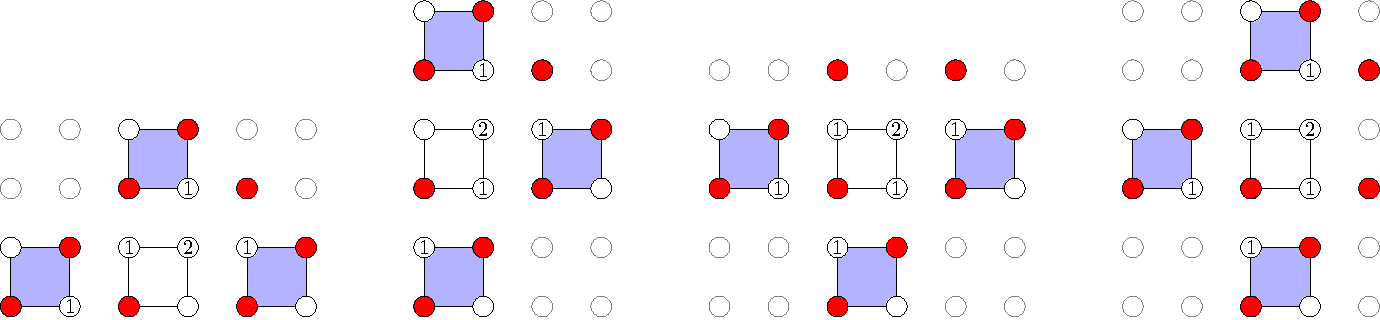
\includegraphics[width=\textwidth]{figures/6/tile_infection.pdf}
\caption{The four configurations of blue tiles leading to infection.}
\label{fig:tile_infection}
\end{figure} 

We have shown that the existence of a perfect lethal set on $[a_1] \times [a_2]$ implies the existence of a perfect lethal set on $[(a_1-1)/2] \times [(a_2-1)/2)]$. Proposition \ref{prop:odd_by_odd} mandates that all perfect lethal sets on $[a_1] \times [a_2]$ be odd-by-odd. Together, these statements require that $a_1 = 2^{k_1}-1$ and $a_2 = 2^{k_2}-1$ for some $k_1,k_2 > 0$, respectively. By repeated applications of Lemma \ref{lem:blue_lethal}, we ultimately obtain a grid $[a_0] \times [1]$ that admits a perfect lethal set. Clearly, the only such grid is the single vertex $[1]$. We therefore conclude that the only two-dimensional grids that admit perfect lethal sets under 3-neighbor percolation are square grids of the form $[2^n-1]^2$. A construction that achieves this is published in Benevides et al \cite{benevides}, and reproduced below.

\subsection{Purina}

We refer to this construction colloquially as the Purina construction, due to the similarly between its instance on the $(3,3,1)$ grid and the logo of the pet food brand. No funding has been offered, but we are open to the possibility. A more extensive discussion on this pattern can be found in \cite{benevides:2021}.

\begin{con}
\label{con:purina}
All grids of the form $(2^n-1, 2^n-1, 1)$ are perfect.
\end{con}

\begin{figure}[]
\centering

\includegraphics[width=0.1\textwidth]{figures/7/3x3x1.pdf}
\caption{A perfect percolating set for $(3,3,1)$.}
\label{fig:3x3x1}
\end{figure} 

\begin{proof}
This is a recursive construction built from the base component piece shown in Figure \ref{fig:3x3x1}. Note that this $(3,3,1)$ construction is lethal under the 3-neighbor bootstrap process, and that it meets the surface area bound:
$$\frac{1}{3} \cdot (ab+bc+ca) = \frac{1}{3} \cdot (9 + 3 + 3) = 5.$$
For larger grids of size $(2^n-1, 2^n-1, 1)$, join four copies of $(2^{n-1}-1, 2^{n-1}, 1)$ about two perpendicular corridors, and infect the vertex at their intersection (Figure \ref{fig:15x15x1}). Observe that the resulting set is lethal: each of the four smaller grids is lethal by hypothesis, and the remaining vertices induce a forest with disconnected boundary points, which percolates by Proposition \ref{prop:immune_regions}. Furthermore, note that
\begin{align*}
\text{S.A.}(2^n-1,2^n-1,1) &= \frac{1}{3} \cdot (2^{2n}-1) \\
&= 4 \cdot \frac{1}{3} \cdot (2^{2n-2} -1) + 1 = 4 \cdot \text{S.A.}(2^{n-1}-1, 2^{n-1}, 1) + 1,
\end{align*}
and therefore this construction is perfect.
\end{proof}

\begin{figure}[]
\centering

\includegraphics[width=0.6\textwidth]{figures/7/15x15x1.pdf}
\caption{A perfect percolating set for $(15,15,1)$.}
\label{fig:15x15x1}
\end{figure} 

Although the only two-dimensional grids that admit perfect lethal sets under 3-neighbor percolation are square grids of the form $[2^n-1]^2$, there is at least one family of two-dimensional grids that admits optimal lethal sets. We examine these grids in the following chapter, and note that their existence is of particular value in our analysis of other infinite families of grids that admit perfect lethal sets. 



\chapter{Constructions}

\section{Introduction}

In this chapter, we present diagrammed proofs of grids that admit optimal and perfect lethal sets under the 3-neighbor process. The proofs are organized by the thickness of the grid. All constructions in the following sections belong to infinite families of grids. We use two strategies in our analysis of these constructions, dependent on the parity of the grid. 

We examine families of the form $(0,1,1) \pmod 2$ by region, and observe that certain regions can be expanded to arbitrarily large sizes without adversely affecting the spread of infection. In particular, we split these grids into components $A,B,X$, where $A$ and $B$ bookend a central, repeating segment $X$. Our discussion will make use of the following definition and lemma:

\begin{defn}
For a grid $G=[a_1] \times [a_2] \times [a_3]$, define the $k$th \emph{level} of $G$ as the subgraph $L_k = [a_1] \times [a_2] \times \{k\}$, for $k \in [a_3]$. 
\end{defn}

\begin{lem}
\label{lem:2_neighbor_levels}
Let $G=[a_1] \times [a_2] \times [a_3]$ and let $L_k$ be the $k$th level of $G$. Suppose all vertices in $L_k$ are infected. Then any lethal set in $L_{k+1}$ (resp. $L_{k-1}$) under the 2-neighbor process is lethal in $G[V(L_{k}) \cup V(L_{k+1})]$ (resp. $G[V(L_{k-1}) \cup V(L_{k})]$) under the 3-neighbor process. 
\end{lem}

\begin{proof}
Each vertex $v \in L_{k+1} \cup L_{k-1}$ has an infected neighbor in $L_k$. Therefore, if $v$ has two infected neighbors in its own level, it has at least 3 infected neighbors in $G$. 
\end{proof}

Proofs of the lethality of the remaining families all leverage Lemma \ref{lem:walls}. As a consequence, their argumentative structure remains broadly the same, even as the constructions themselves appear quite different. We shall outline this structure here, before examining the specific proofs. 

We begin by demonstrating that the grid $G=(a_1,a_2,a_3)$ admits a manifold $M$. Recall from Corollary \ref{cor:walls} that a manifold on $G$ is the union of faces
$$F_{1,k_1} \cup F_{2,k_2} \cup F_{3,k_3}$$
for some $k_i \in [a_i]$. To show that a particular subset $M$ of $V(G)$ is a manifold, we identify the regions $R_1, \dots, R_n$ that partition $V(G) \setminus M$ and are flanked by three perpendicular walls. In our diagrams, these regions are represented by the volumes bordered by three perpendicular blue, green, and red walls. We then identify a proper unfolding $H$ of $M$ and show that $H$ admits a lethal set $A$, where $|A| = \text{SA}(G)$. Finally, we apply Corollary \ref{cor:walls} to prove that $G$ is perfect. 

%We shall call a thickness \emph{semi-complete} if all divisibility cases are optimal. We present some useful definitions and lemmas.

\section{Thickness 1}

We present a construction that is optimal on all grids $(a,b,1)$, where $a \equiv 5 \pmod 6$, $b \equiv 1 \pmod 2$, and $a,b \geq 5$. As such grids constitute non-divisibility cases, this construction is not perfect. However, by leveraging Lemma \ref{lem:unfolded_cube}, we shall see that it can be used to obtain perfect lethal sets on certain grids of thickness 3. 

As indicated by Proposition \ref{prop:immune_regions}, a fundamental characteristic of lethal sets $A_0$ is the presence of an initially uninfected corridor, bounded by walls of infection. This structure is apparent in the second diagrams of Figures \ref{fig:15x15x1} and \ref{fig:11x13x1} in the previous chapter. These corridors correspond to forests in the complement $G[\overline{A_0}]$ of $A_0$. In this section, we provide a general method for constructing such corridors in $(a, b, 1)$ grids where $a \equiv 5 \pmod 6$ and $b \equiv 1 \pmod 2$.

% WITH THE EXCEPTION OF WIDTH 3!!!!!
% WIDTH >= 5
\begin{con}
\label{con:snake}
All grids of the form $(a,b,1)$, $a \equiv 5 \pmod 6$, $b \equiv 1 \pmod 2$, and $a,b \geq 5$ are optimal.
\end{con}

\begin{proof}
For grids of the form $(a,b,1)$, $a \equiv 5 \pmod 6$, $b \equiv 1 \pmod 2$, we construct an optimal infected set and show that it is lethal by Proposition \ref{prop:immune_regions}. For the base case, consider the $(5,5,1)$ grid $G$ illustrated in Figure \ref{fig:5x5x1}. Observe that this construction is optimal. Now consider the grid $G'$ resulting from the insertion of a $(5, 2k, 1)$ block, as shown in Figure \ref{fig:5x13x1}. Note that the subgraph induced by the uninfected vertices of $G'$ satisfies the conditions of Proposition \ref{prop:immune_regions}. Furthermore, note that if any $(5, n, 1)$ grid is optimal, the $(5,n+2,1)$ grid resulting from such a construction has surface area bound $\text{S.A.}(5,n,1) + 4$, which agrees with the number of infected vertices.

\begin{figure}[]
\centering

\includegraphics[width=0.15\textwidth]{figures/7/5x5x1.pdf}
\caption{An optimal percolating set for $(5,5,1)$.}
\label{fig:5x5x1}
\end{figure} 

\begin{figure}[]
\centering
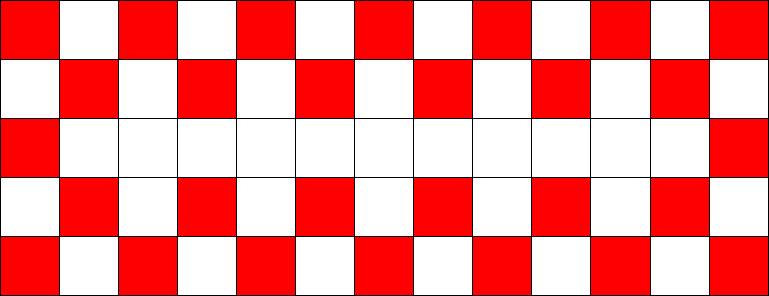
\includegraphics[width=0.5\textwidth]{figures/7/5x13x1.pdf}
\caption{An optimal percolating set for $(5,13,1)$.}
\label{fig:5x13x1}
\end{figure} 

To extend this construction in the vertical direction, we introduce a kink in the snaking infection. This kink requires six rows to produce a repeating pattern. The structure of this design is shown in Figure \ref{fig:11x13x1}. For grids of smaller width, the same construction gives optimal percolating sets; however, the snaking pattern is increasingly difficult to recognize in thin grids.
\end{proof}

\begin{figure}[]
\centering

\includegraphics[width=0.6\textwidth]{figures/7/11x13x1.pdf}
\caption{An optimal percolating set for $(11,13,1)$.}
\label{fig:11x13x1}
\end{figure} 

% Maybe other (divisibility) constructions that percolate at 1 over the bound (if they exist)?

\section{Thickness 2}

We examine four infinite families of perfect grids and show that each has a manifold that admits a lethal set of perfect size. We note that such lethal sets are likely to exist for nearly all divisibility cases in thickness two; however, constructions are elusive and those presented here are sufficient to prove the main result of this thesis.

% (3 mod 6, 3, 2)
\begin{con}
All $(a,3,2)$ grids with $a \equiv 3 \pmod 6$ and $a >3$ are perfect. 
\end{con}

\begin{proof}
%(This construction is the same as the previous one, except the the final four columns are augmented slightly to accommodate the $0 \pmod 3$ requirement. Instead of deriving a proper unfolding, it is probably easier to simply show that this small change is sufficient to guarantee lethality, and agrees with the S.A. bound.)

%We proceed by induction. Consider the grid $G=(9,3,2)$, and let $A_t$ be the set of infected vertices at time-step $t$ (see Figure \ref{fig:9x3x2}). We show that $A_0$ is lethal on $G_1$ and $G_2$. Observe that after one time-step, the subgraph $G_1[\overline{A_1}]$ is a forest connected to the border of $G_1$, and so by Proposition \ref{prop:immune_regions}, $A_0$ is lethal on $G_1$. Since $A_0$ is lethal on $G_1$, by Lemma \ref{lem:2_neighbor_levels}, it is sufficient to prove that $A_0$ is lethal on $G_2$ under the 2-neighbor bootstrap process. Figure \ref{fig:9x3x1} illustrates the key steps of this process, starting at $t=1$. Infection spreads down rows delineated by red arrows, ultimately infecting all vertices in $G_2$. We conclude that $A_0$ is lethal on $G$ under the 3-neighbor process.

%Let $A = \{1\} \times [3] \times [2]$, $B = \{8,9\} \times [3] \times [2]$ and $X = \{2,3,4,5,6,7\} \times [3] \times [2]$ be components of $G$ (see Figure \ref{fig:9x3x2}). Denote by $AX^kB$ the graph obtained by inserting $k$ copies of $X$ between components $A$ and $B$. Let $A_0^k$ be a lethal set on $AX^kB$. We show that $A_0^{k+1}$ is lethal on $AX^{k+1}B$. 

Let $G=(6k+3,3,2)$ be a grid such that $k>0$. Let $A = \{1\} \times [3] \times [2]$, $B = \{6k+2, 6k+3\} \times [3] \times [2]$, and $X_i = \{6i+2,6i+3,6i+4,6i+5,6i+6,6i+7\} \times [3] \times [2]$ for $i \in [k - 1] \cup \{0\}$, be components of $G$. Denote by $AX^kB$ the union of components $A \cup X_0 \cup \dots \cup X_{k-1} \cup B$, and note that $G=AX^kB$. Let $A_t^k \subseteq V(G)$ be the set of infectious vertices in $G$ at time $t$, and suppose that each $X_i$ contains the same pattern of infected vertices (see Figure \ref{fig:9x3x2}). We show that $A_0^k$ is lethal and perfect. 

Consider the union of components $AX^k = A \cup X_0 \cup \dots \cup X_{k-1}$ (see Figure \ref{fig:19x3x2}). Let $L_1$ and $L_2$ be the top and bottom levels $AX^k$, respectively. Observe that after one time-step, the subgraph $L_1[\overline{A_1^k}]$ is a forest connected to the border of $L_1$, and so by Proposition \ref{prop:immune_regions}, $A_0^k$ is lethal on $L_1$. 

Now consider $G$ and observe that the top level becomes fully infected (see Figure \ref{fig:21x3x2}). Therefore, by Lemma \ref{lem:2_neighbor_levels}, it is sufficient to prove that $A_0^k$ is lethal on the bottom level under the 2-neighbor bootstrap process. Figure \ref{fig:9x3x1} illustrates the key steps of this process on the smaller grid $AXB$, starting at $t=1$. Infection spreads down rows delineated by red arrows, ultimately infecting all vertices in the bottom level. We conclude that $A_0^k$ is lethal on $G$ under the 3-neighbor process.

To prove that $A_0^k$ is perfect, observe that $|A_0^k| = 3 + 10k + 4$. The surface area bound for $G=(6k+3,3,2)$ is given by
$$\frac{(3)(6k+3) + (3)(2) + (2)(6k+3)}{3} = \frac{30k + 21}{3} = 10k+7.$$
Since these two values are equal, $A_0^k$ is tight and lethal, and therefore perfect.
\end{proof}

\begin{figure}[]
\centering
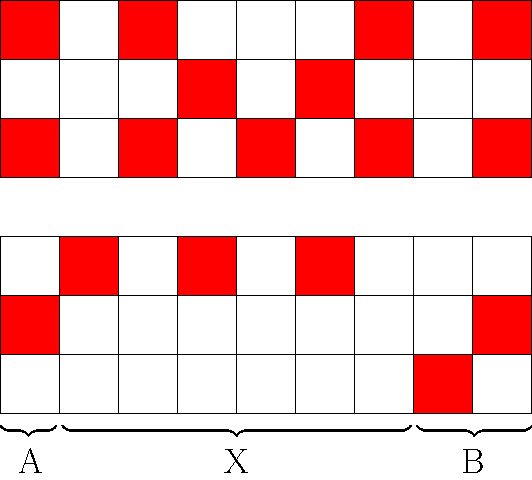
\includegraphics[width=0.3\textwidth]{figures/7/3x9x2.pdf}
\caption{The components $A$, $X$, $B$ on $G=AXB$ with infectious set $A_0$.}
\label{fig:9x3x2}
\end{figure} 

\begin{figure}[]
\centering
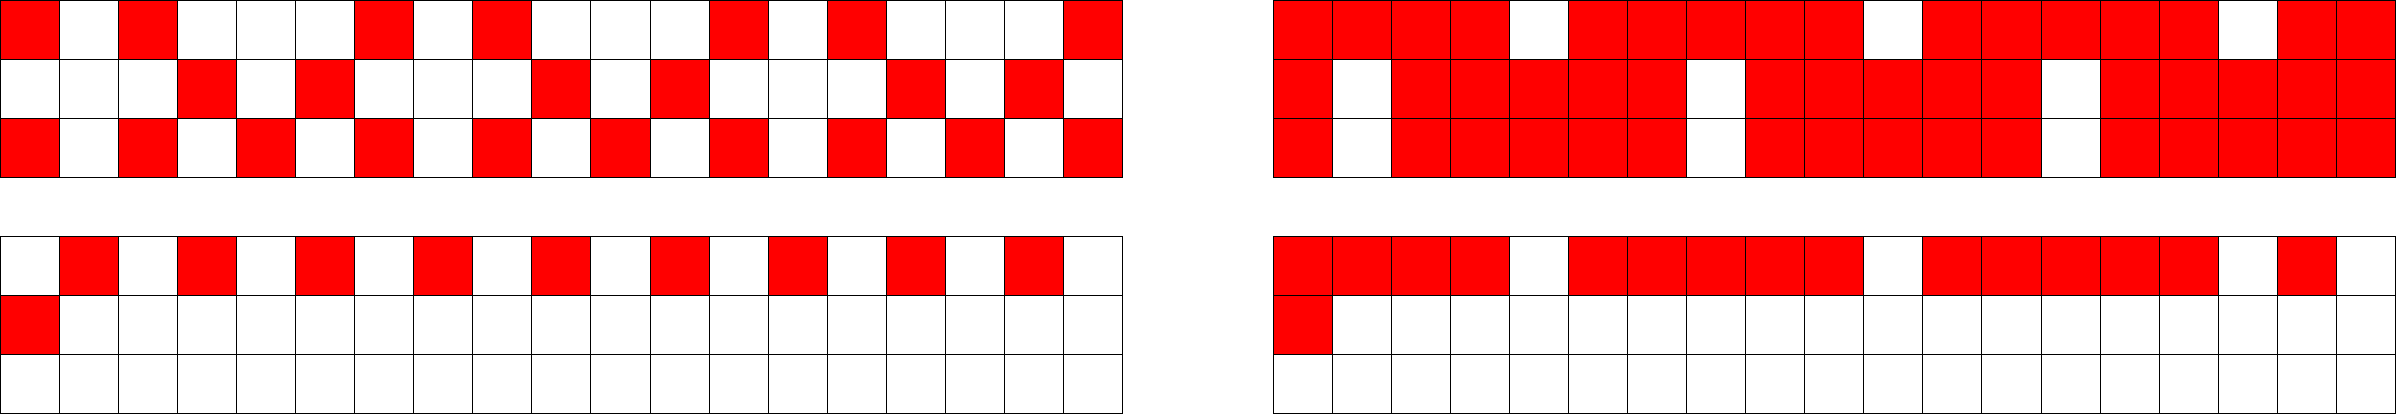
\includegraphics[width=0.8\textwidth]{figures/7/3x19x2.pdf}
\caption{An infection on $AX^3$, $t=0$ and $t=1$.}
\label{fig:19x3x2}
\end{figure} 

\begin{figure}[]
\centering
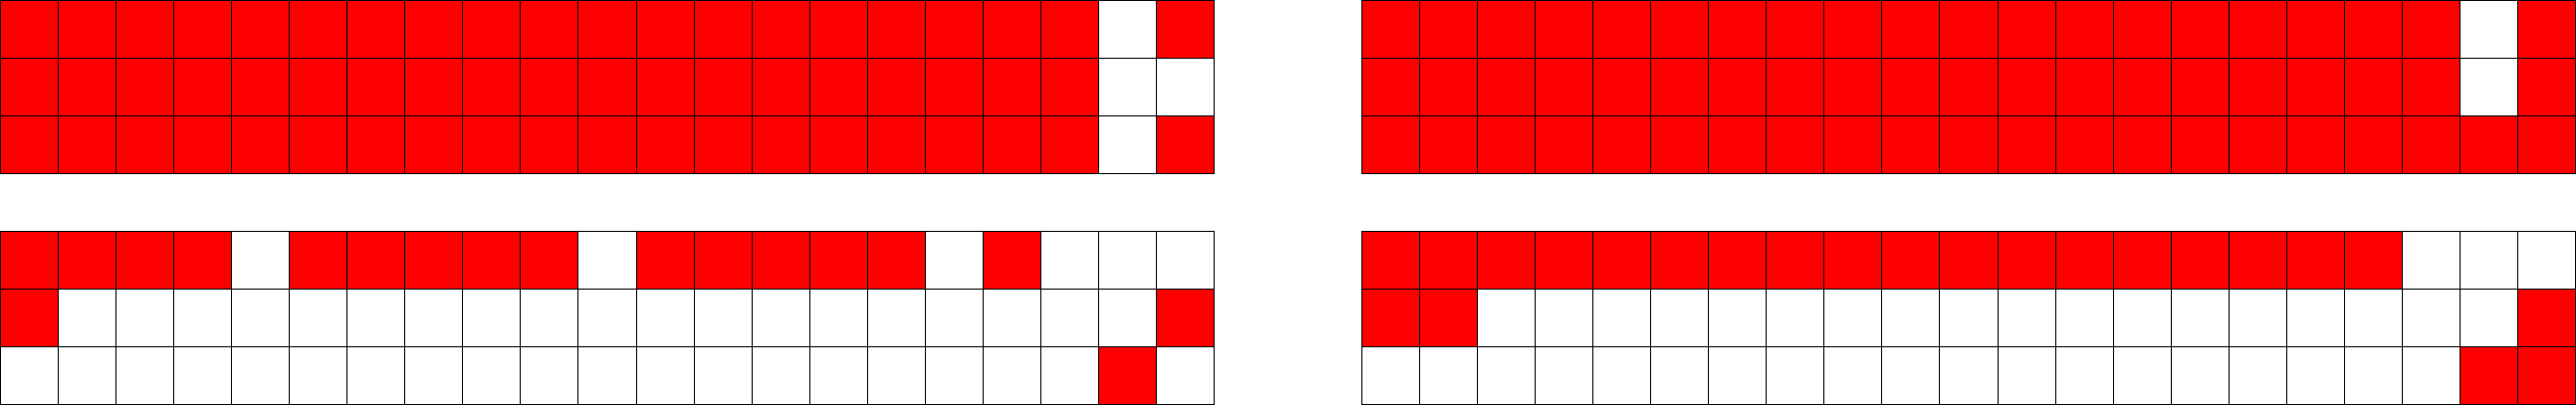
\includegraphics[width=0.8\textwidth]{figures/7/3x21x2.pdf}
\caption{An infection on $G$.}
\label{fig:21x3x2}
\end{figure} 

\begin{figure}[]
\centering
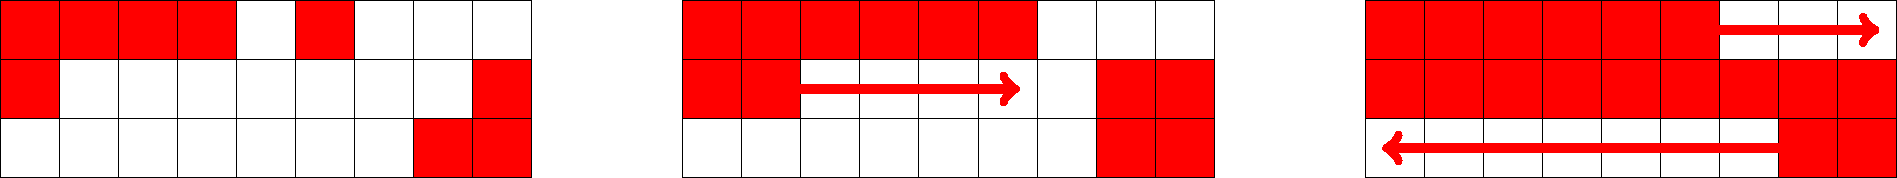
\includegraphics[width=0.8\textwidth]{figures/7/3x9x1.pdf}
\caption{The 2-neighbor process on $(9,3,1)$ for $t=1$, $t \in \{2,3,4,5,6\}$, and $t \in \{7,8,9,10,11,12,13,14\}$.}
\label{fig:9x3x1}
\end{figure} 

\begin{con}
All $(a,3,2)$ grids with $a \equiv 0 \pmod 6$ and $a \geq 6$ are perfect. 
\end{con}

\begin{proof}
Let $G$ be an $(a,3,2)$ grid with $a \equiv 0 \pmod 6$ and $a \geq 6$, and let $M$ be a manifold of $G$ and $H$ be its proper unfolding (see Figure \ref{fig:3x12x2_manifold}). Observe that $M$ is indeed a manifold: it partitions $V(G) \setminus M$ into two sets $R_1$ and $R_2$, both bounded by mutually orthogonal red, green, and blue faces (see Figure \ref{fig:3x12x2_manifold_a}). Furthermore, note that $H$ is obtained from $M$ by cutting along seams between red and green faces, and flattening the figure. It follows that $H$ is a proper unfolding of $G$. 

Let $X_1, \dots, X_k$ be the repeated components of $H$. Denote by $X$ the union of these components. Let $A_t \subseteq V(H)$ be the set of infectious vertices in $H$ at time $t$, and suppose that each $X_i$ contains the same pattern of infected vertices (see Figure \ref{fig:3x12x2_unfolded_lethal}). We show that $A_0$ is lethal and perfect.

Consider an initial infection $A_0$ of $H$ (see Figure \ref{fig:3x12x2_unfolded_lethal}). Observe that $A_0$ infects all vertices of $X$ by Proposition \ref{prop:immune_regions}. We show that the remaining healthy vertices of $H$ become infected. Consider re-folding $H$, and note that the two cells marked with an ``X" in $H$ represent the same cell in $G$. This is enough to infect the remaining regions of $H$, and by Corollary \ref{cor:walls}, $A_0$ is lethal on $G$. 
%Furthermore, observe that $G$ can be extended in the $x$ direction by repeated insertions of the component $X$ (see Figure \ref{fig:3x12x2}). This process does not affect the structure of $H$, and Proposition \ref{prop:immune_regions} again guarantees lethality.

To prove that $A_0$ is perfect, observe that $|A_0| = 4 + 10k + 8 = 10k +12$. The surface area bound for $G=(6k+6,3,2)$, where $k$ is the number of repeated components $X$, is given by
$$\frac{(3)(6k+6) + (3)(2) + (2)(6k+6)}{3} = \frac{30k + 36}{3} = 10k+12.$$
Since these two values are equal, $A_0$ is tight and lethal, and therefore perfect.
\end{proof}

% (0 mod 6, 3, 2)

\begin{figure}[]
\centering
\begin{subfigure}{0.45\textwidth}
	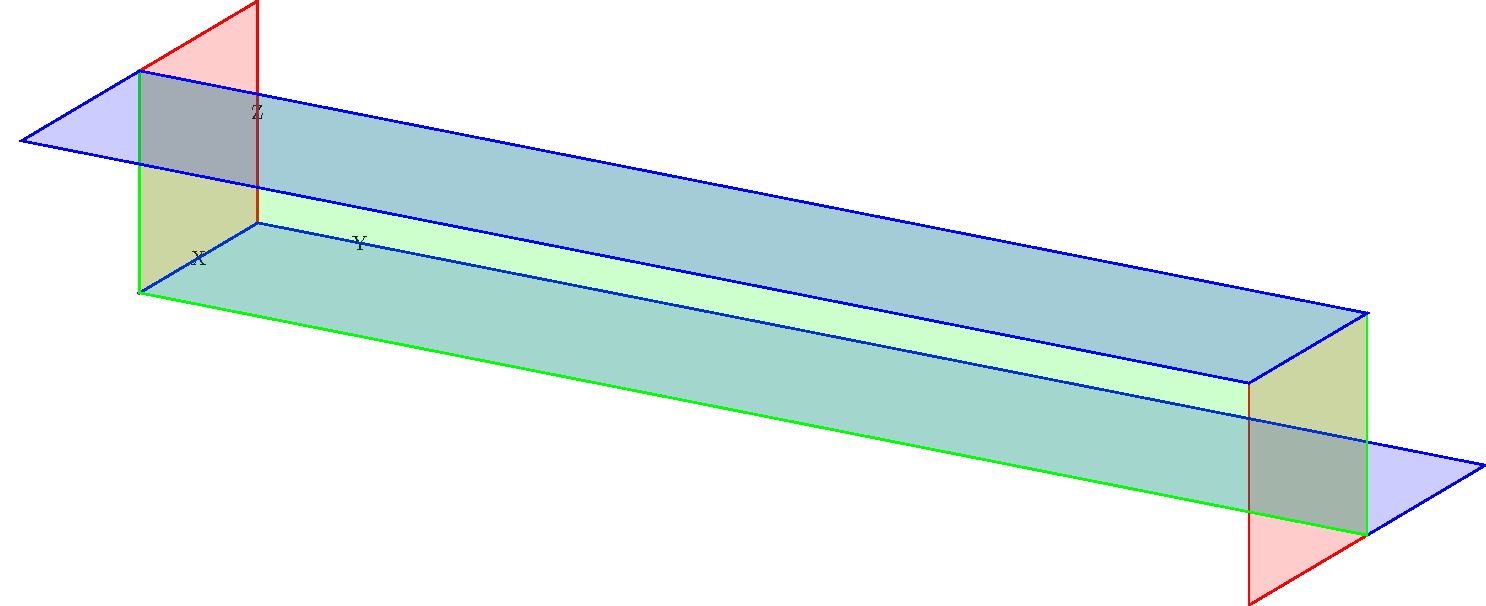
\includegraphics[width=\textwidth]{figures/7/3x12x2_manifold_3d.pdf}
	\caption{A manifold of $G= (3,12,2)$.}
	\label{fig:3x12x2_manifold_a}
\end{subfigure} \hfill%
\begin{subfigure}{0.45\textwidth}
	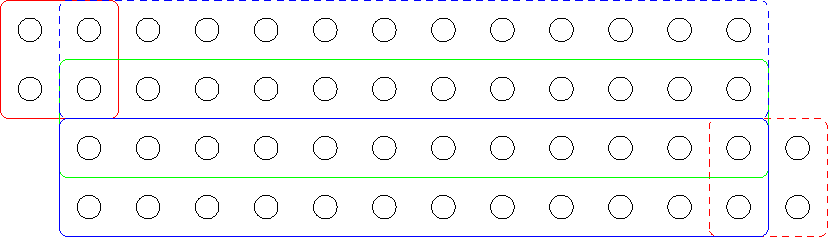
\includegraphics[width=\textwidth]{figures/7/3x12x2_manifold.pdf}
	\caption{A proper unfolding of $G$.}
	\label{fig:3x12x2_manifold_b}
\end{subfigure}
\caption{A proper unfolding of $G= (3,12,2)$. Colored rectangles indicate faces of $G$. Dashed lines indicate that cells appear on different layers. }
\label{fig:3x12x2_manifold}
\end{figure} 

\begin{figure}[]
\centering
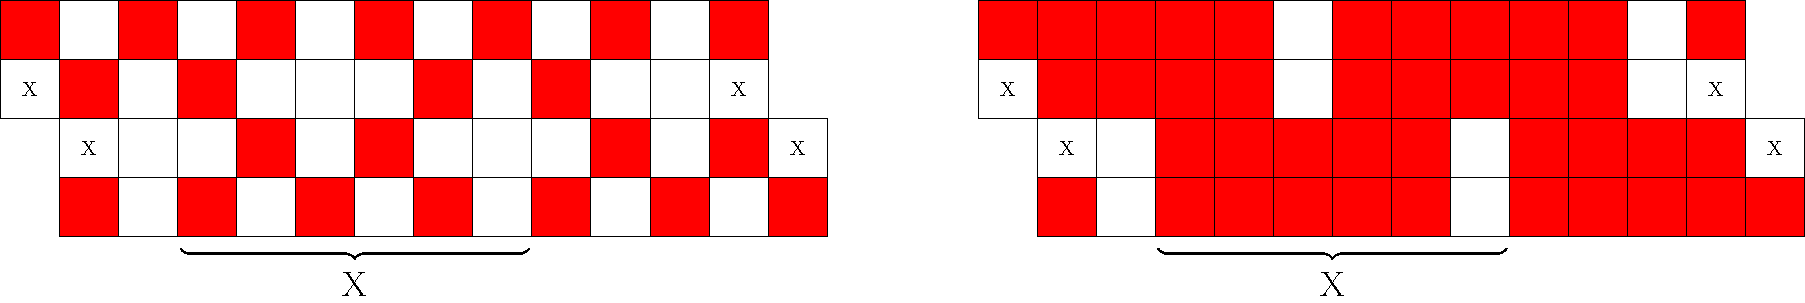
\includegraphics[width=0.8\textwidth]{figures/7/3x12x2_unfolded_lethal.pdf}
\caption{A lethal set on $H$ showing the repeated component $X$ ($t=1$ and $t=2$).}
\label{fig:3x12x2_unfolded_lethal}
\end{figure} 

\begin{figure}[]
\centering
\includegraphics[width=0.8\textwidth]{figures/7/3x12x2.pdf}
\caption{A perfect lethal set for $(3,12,2)$ with component $X$.}
\label{fig:3x12x2}
\end{figure} 

% (2 mod 6, 5 mod 6, 2)

% a,b, MUST BE A CERTAIN SIZE
\begin{con}
All $(a,b,2)$ grids with $a,b \in \{2,5\} \pmod 6$, $a \neq b \pmod 6$, and $a,b > 2$ are perfect. 
\end{con}

\begin{proof}
Let $G$ be an $(a,b,2)$ grid with $a,b \in \{2,5\} \pmod 6$, $a \neq b \pmod 6$, and $a,b > 2$, and let $M$ be a manifold of $G$ and $H$ be its proper unfolding (Figure \ref{fig:11x20x2_manifold}). Note that $M$ partitions the vertices of $V(G) \setminus M$ into two disjoint sets $R_1$ and $R_2$, both bounded by mutually orthogonal red, green, and blue faces. Note, also, that $H$ is obtained from $M$ by cutting along seams between red and green faces, and flattening the figure. Therefore, $H$ is a proper unfolding of $G$. 

Let $X_1, \dots, X_{k_1}$ be the repeated components of $H$ in the $x$-direction, and $Y_1, \dots, Y_{k_2}$ be the repeated components of $H$ in the $y$-direction (see Figure \ref{fig:18x16x1_unfolded_lethal}). Denote by $X \times Y$ the union of these components. Let $A_t \subseteq V(H)$ be the set of infectious vertices in $H$ at time $t$, and suppose that for $i \in [k_1] \setminus \{1,k_1\}$ and $j \in [k_2]$, each $X_i \times Y_j$ contains the same pattern of infected vertices (see Figure \ref{fig:XiYj}). We show that $A_0$ is lethal and perfect.

Consider the initial infection $A_0$ of $H$ as shown in Figure \ref{fig:18x16x1_unfolded_lethal}. Observe that $A_0$ infects all vertices of $X\times Y$ by Proposition \ref{prop:immune_regions}. We show that the remaining healthy vertices of $H$ become infected. The individual vertices in the rightmost column of $H$ are infected by Proposition \ref{prop:immune_regions}. Consider re-folding $H$, and note that the two cells marked with an ``X" in $H$ represent the same cell in $G$. This is enough to infect the remaining regions of $H$, and by Corollary \ref{cor:walls}, $A_0$ is lethal on $G$. 

To prove that $A_0$ is perfect, observe that for $i \in [k_1] \setminus \{1\}$ and $j \in [k_2]$, each $X_i \times Y_j$ block contains exactly 12 infected vertices. For $j \in [k_2 -1]$, $X_1 \times Y_j$ contains 11 infected vertices, and $X_1 \times Y_{k_2}$ contains 12 infected vertices. In total, the component $X \times Y$ contains exactly 
$$12(k_1-1)(k_2) + 11(k_2-1) + 12$$
initially infected vertices. Of the remaining vertices in $H$, $14(k_1) - 1 +9(k_2) + 8$ are infected. Therefore, 
\begin{align*}
|A_0| &= 12(k_1-1)(k_2) + 11(k_2-1) + 12+14(k_1) - 1 +9(k_2) + 8 \\
&= 12k_1k_2 + 14k_1 + 8k_2 +8.
\end{align*}
The surface area bound for $G=(6k_1+2,6k_2+5,2)$ is given by
\begin{align*}
SA(6k_1+2,6k_2+5,2) &= \frac{(6k_1+2)(6k_2 + 5) + (6k_2+5)(2) + (2)(6k_1+2)}{3} \\
&= \frac{36(k_1)(k_2) +42k_1 +24k_2 + 24}{3} \\
&= 12k_1k_2 +14k_1+8k_2+8.
\end{align*}
Since these two values are equal, $A_0$ is tight and lethal, and therefore perfect.
\end{proof}

\begin{figure}[]
\centering
\begin{subfigure}{0.45\textwidth}
	\includegraphics[width=\textwidth]{figures/7/11x20x2_manifold_3d.pdf}
	\caption{A manifold of $G= (11,20,2)$.}
	\label{}
\end{subfigure} \hfill%
\begin{subfigure}{0.45\textwidth}
	\includegraphics[width=\textwidth]{figures/7/11x20x2_manifold.pdf}
	\caption{A proper unfolding of $G$.}
	\label{}
\end{subfigure}
\caption{A proper unfolding of $G= (11,20,2)$. Colored rectangles indicate faces of $G$. Dashed lines indicate that cells appear on different layers. }
\label{fig:11x20x2_manifold}
\end{figure} 

\begin{figure}[]
\centering
\includegraphics[width=0.8\textwidth]{figures/7/18x16x1_unfolded_lethal.pdf}
\caption{A percolating set on the proper unfolding of $G= (17,14,2)$.}
\label{fig:18x16x1_unfolded_lethal}
\end{figure}

\begin{figure}[]
\centering
\includegraphics[width=0.6\textwidth]{figures/7/17x14x2.pdf}
\caption{A perfect percolating set for $(17,20,2)$.}
\label{fig:11x20x2}
\end{figure} 

\begin{figure}[]
\centering
\includegraphics[width=0.12\textwidth]{figures/7/XiYj.pdf}
\caption{A block $X_i \times Y_j$.}
\label{fig:XiYj}
\end{figure} 

% (3 mod 6, 0 mod 6, 2) 

% a,b MUST BE A CERTAIN SIZE
\begin{con}
All $(a,b,2)$ grids with $a,b \in \{0,3\} \pmod 6$, $a \neq b \pmod 6$ and $a,b, \geq 6$ are perfect. 
\end{con}

\begin{proof}
Let $G$ be an $(a,b,2)$ grid with $a,b \in \{0,3\} \pmod 6$, $a \neq b \pmod 6$, and $a,b \geq 6$, and let $X_1, \dots, X_{k_1}$ be the repeated components of $G$ in the $x$-direction, and $Y_1, \dots, Y_{k_2}$ be the repeated components of $G$ in the $y$-direction (see Figure \ref{fig:12x15x2}). Denote the union of these components by $X \times Y$. Let $A_t \subseteq V(H)$ be the set of infectious vertices in $G$ at time $t$, and suppose that for $i \in [k_1]$ and $j \in [k_2]$, each $X_i \times Y_j$ contains the same pattern of infected vertices (see Figure \ref{fig:12x15x2}). We show that $A_0$ is lethal and perfect.

Let $L_1$ and $L_2$ be the top and bottom layers of $G$, respectively. Observe that after one time-step, the subgraph of $L_1$ induced by the uninfected vertices of $\cup Y_i$ is both acyclic and contains no border-to-border paths. Therefore, by Proposition \ref{prop:immune_regions}, $A_0$ is lethal in $(\cup Y_i) \cap L_1$. 

Consider these observations in the context of $G$. Figure \ref{fig:12x15x2_L1} shows that after 5 additional time-steps, the remaining healthy vertices in $L_1$ form two corridors, marked by red arrows. The vertices in the upper corridor are infected by Proposition \ref{prop:immune_regions}, and those in the lower corridor are infected by Lemma \ref{lem:2_neighbor_levels}. Therefore, all vertices of $L_1$ become infected. Furthermore, the infected vertices in $L_2$ form a lethal set under the 2-neighbor process, and so, by Lemma \ref{lem:2_neighbor_levels}, we conclude that $A_0$ is lethal on $G$ under the 3-neighbor process.

To prove that $A_0$ is perfect, observe that for $i \in [k_1]$ and $j \in [k_2]$, each $X_i \times Y_j$ block contains exactly 12 infected vertices, and so the total number of infected vertices in $X \times Y$ is $12k_1k_2$. 

Of the remaining vertices in $G$, $16k_1+22k_2+28$ are infected. Therefore,
$$|A_0| = 12k_1k_2 + 16k_1+22k_2+28.$$ 
The surface area bound for $G=(6k_1+9,6k_2+6,2)$ is given by
\begin{align*}
SA(6k_1+9,6k_2+6,2) &= \frac{(6k_1+9)(6k_2+6) + (6k_2+6)(2) + (2)(6k_1+9)}{3} \\
&= \frac{36k_1k_2+ 48k_1 + 66k_2 + 84}{3} \\
&= 12k_1k_2+16k_1+22k_2+28.
\end{align*}
Since these two values are equal, $A_0$ is tight and lethal, and therefore perfect.
\end{proof}

\begin{figure}[]
\centering
\includegraphics[width=0.8\textwidth]{figures/7/12x15x2.pdf}
\caption{A perfect percolating set for $(12,21,2)$.}
\label{fig:12x15x2}
\end{figure} 

\begin{figure}[]
\centering
\includegraphics[width=0.6\textwidth]{figures/7/12x15x2_L1_numbered_heatmap.pdf}
\caption{A perfect percolating set for $(12,21,2)$.}
\label{fig:12x15x2_L1}
\end{figure} 

We note that it is possible to examine grids of the form described above using a folding argument, \emph{if} they are at least as large as $(12,21,2)$. However, such a process omits an infinite number of smaller grids. Nevertheless, the construction is of interest, and the grid and corresponding unfolded net are given in Figures \ref{fig:12x21x2}, \ref{fig:12x21x2_unfolded} and \ref{fig:12x21x2_unfolded_lethal} in the Appendix. 

% COMMENT
% COMMENT
% COMMENT
\begin{comment}

\begin{figure}[]
\centering
\includegraphics[width=0.8\textwidth]{figures/7/12x21x2.pdf}
\caption{A perfect percolating set for $(12,21,2)$.}
\label{fig:12x21x2}
\end{figure} 

\begin{figure}[]
\centering
\begin{subfigure}{0.45\textwidth}
	\includegraphics[width=\textwidth]{figures/7/12x21x2_manifold_3d.pdf}
	\caption{A manifold of $G= (12,21,2)$.}
	\label{}
\end{subfigure} \hfill%
\begin{subfigure}{0.45\textwidth}
	\includegraphics[width=\textwidth]{figures/7/12x21x2_unfolded.pdf}
	\caption{A proper unfolding of $G$.}
	\label{}
\end{subfigure}
\caption{A proper unfolding of $G= (12,21,2)$. Colored rectangles indicate faces of $G$. Dashed lines indicate that cells appear on different layers. }
\label{fig:12x21x2_unfolded}
\end{figure} 

\begin{figure}[]
\centering
\includegraphics[width=0.8\textwidth]{figures/7/12x21x2_unfolded_lethal.pdf}
\caption{A percolating set on the proper unfolding of $G= (12,21,2)$.}
\label{fig:12x21x2_unfolded_lethal}
\end{figure} 

\end{comment}
% COMMENT
% COMMENT
% COMMENT

\section{Thickness 3}

\begin{con}
All $(a,3,3)$ grids $G$ with $a \equiv 0 \pmod 2$ and $a > 2$ are perfect. 
\end{con}

\begin{proof}
Let $G=(2k,3,3)$ be a grid such that $k > 1$. Let $A = \{1,2,3\} \times [3] \times [3]$, $B = \{2k\} \times [3] \times [3]$, and $X_i = \{2i+2,2i+3\} \times [3] \times [3]$ for $i \in [k-2]$, be components of $G$. Denote by $AX^kB$ the union of components $A \cup X_1 \cup \dots \cup X_{k} \cup B$, and note that $G=AX^kB$. Let $A_t^k \subseteq V(G)$ be the set of infectious vertices in $G$ at time $t$, and suppose that each $X_i$ contains the same pattern of infected vertices (see Figure \ref{fig:3x6x3}). We show that $A_0^k$ is lethal and perfect. 

Consider the union of components $AX^k = A \cup X_1 \cup \dots \cup X_{k}$ (see Figure \ref{fig:3x13x3}). Let $L_1$, $L_2$ and $L_3$ be the top, middle and bottom levels of $AX^k$, respectively. Observe that after one time-step, the subgraph of $L_2 \setminus \{2k-1\} \times [3] \times \{2\}$ induced by $\overline{A_0^k}$ is acyclic with no border-to-border vertices, and so by Proposition \ref{prop:immune_regions}, $A_0^k$ infects all vertices of $L_2$ apart from those in the rightmost column (labeled ``X"; see Figure \ref{fig:3x13x3}). Therefore, by Lemma \ref{lem:2_neighbor_levels}, all vertices in $L_1$ apart from the rightmost column (labeled ``Y") become infected by the 2-neighbor process. Similarly, the red arrow in Figure \ref{fig:3x13x3}) shows the path of infection in $L_3$. 

Consider these observations in the context of $G$. Figure \ref{fig:3x14x3} shows that it takes 7 additional time-steps to fully infect $L_1$ and $L_2$. By Lemma \ref{lem:2_neighbor_levels}, the remaining healthy vertices in $L_3$ become infected. We therefore conclude that $A_0^k$ is lethal on $G$ under the 3-neighbor process.

To prove that $A_0^k$ is perfect, observe that $|A_0^k| = 8 + 4(k-2) + 3=4k+3$. The surface area bound for $G=(2k,3,3)$ is given by
$$\frac{(2k)(3) + (3)(3) + (3)(2k)}{3} = \frac{12k + 9}{3} = 4k+3.$$
Since these two values are equal, $A_0^k$ is tight and lethal, and therefore perfect.
\end{proof}

\begin{figure}[]
\centering
\includegraphics[width=0.2\textwidth]{figures/7/3x6x3.pdf}
\caption{The components $A$, $X$, $B$ on $G=AXB$ with infectious set $A_0$.}
\label{fig:3x6x3}
\end{figure} 

\begin{figure}[]
\centering
\includegraphics[width=0.8\textwidth]{figures/7/3x13x3.pdf}
\caption{An infection on $AX^5$, $t=0$ and $t=1$.}
\label{fig:3x13x3}
\end{figure} 

\begin{figure}[]
\centering
\includegraphics[width=0.5\textwidth]{figures/7/3x14x3_numbered_heatmap.pdf}
\caption{An infection on $G$.}
\label{fig:3x14x3}
\end{figure} 

\begin{con}
All $(a,b,3)$ grids $G$ with $a \equiv 3 \pmod 6$, $b \equiv 1 \pmod 2$ and $a,b \geq 3$ are perfect. 
\end{con}

\begin{proof}
Consider the grid $H=(a+2,b+2,1)$, where $a \equiv 3 \pmod 6$ and $b \equiv 1 \pmod 2$. Observe that $H$ admits an optimal percolating set by Construction \ref{con:snake}, and that
$$\text{SA}(a,b,3) = \ceil{\text{SA}(a+2,b+2,1)} - 3.$$
We show that a proper unfolding of $G$ can be obtained from a simple augmentation of $H$. Let $H'$ be the grid obtained by deleting the four vertices in the bottom, right-most corner of $H$ (see Figure \ref{fig:17x25x1_unfolded}). Consider the folding pattern illustrated in Figure \ref{fig:17x25x1_manifold}, and observe that the pairs of vertices adjacent to the deleted region are duplicates of each other. (In other words, consider folding up the red and green regions in Figure \ref{fig:17x25x1_manifold}, and notice that this operation causes vertices to overlap.) Taking this into account, $H'$ percolates by Proposition \ref{prop:immune_regions}. Since $H$ admits an optimal percolating set of size $\ceil{\text{SA}(a+2,b+2,1)}$, and precisely 3 of the vertices deleted from $H$ to obtain $H'$ were infected, it follows that $H'$ admits a perfect lethal set. Finally, by Lemma \ref{cor:walls}, $G$ is perfect.
\end{proof}

\begin{figure}[]
\centering
\includegraphics[width=0.8\textwidth]{figures/7/17x25x1_unfolded.pdf}
\caption{A percolating set on the proper unfolding $H'$ of $G= (15,23,3)$.}
\label{fig:17x25x1_unfolded}
\end{figure}

\begin{figure}[]
\centering
\begin{subfigure}{0.45\textwidth}
	\includegraphics[width=\textwidth]{figures/7/17x25x1_manifold_3d.pdf}
	\caption{A manifold of $G= (15,23,3)$.}
	\label{}
\end{subfigure} \hfill%
\begin{subfigure}{0.45\textwidth}
	\includegraphics[width=\textwidth]{figures/7/17x25x1_manifold.pdf}
	\caption{A proper unfolding of $G$.}
	\label{}
\end{subfigure}
\caption{A proper unfolding of $G= (15,23,3)$. Colored rectangles indicate faces of $G$. }
\label{fig:17x25x1_manifold}
\end{figure} 

\begin{con}
All $(a,4,3)$ grids $G$ with $a \equiv 3 \pmod 6$ and $a \geq 9$ are perfect. 
\end{con}


\begin{proof}
Let $G=(6k+3,4,3)$ be a grid such that $k \geq 1$, and let $X_1, \dots, X_{k}$ be the repeated components of $G$ in the $x$-direction. Denote the union of these components by $X^k$. Let $A_t^k \subseteq V(G)$ be the set of infectious vertices in $G$ at time $t$, and suppose that each $X_i$ contains the same pattern of infected vertices (see Figure \ref{fig:4x15x3}). We show that $A_0^k$ is lethal and perfect. 

Let $L_1$, $L_2$ and $L_3$ be the top, middle and bottom levels of $G$, respectively. Consider $L_3$ at $t=1$ (see Figure \ref{fig:4x15x3}). Observe that the vertices labeled ``X" are infected at $t=2$, and subsequently all vertices in $X^k \cap L_3$ (with the exception of the vertex labeled ``Y") are infected by Proposition \ref{prop:immune_regions}. Additionally, the infected vertices in $L_2$ at $t=1$ are lethal in $X^k \cap L_2$ under the 2-neighbor process, and so by Lemma \ref{lem:2_neighbor_levels}, all vertices of $X^k \cap L_2$ (apart from the one labeled ``Y") are infected.

Consider these observations in the context of $G$. Figure \ref{fig:4x15x3_timesteps} shows that it takes 5 additional time-steps to fully infect $L_2$. By Lemma \ref{lem:2_neighbor_levels}, the remaining healthy vertices in $L_1$ and $L_3$ become infected. We therefore conclude that $A_0^k$ is lethal on $G$ under the 3-neighbor process.

To prove that $A_0^k$ is perfect, observe that for $i \in [k]$, each $X_i$ contains 14 infected vertices. Of the remaining vertices in $G$, 11 are infected. Therefore, $|A_0| = 14k+11$. The surface area bound for $G=(6k+3,4,3)$ is given by
$$\frac{(6k+3)(4) + (4)(3) + (3)(6k+3)}{3} = \frac{42k + 33}{3} = 14k+11.$$
Since these two values are equal, $A_0^k$ is tight and lethal, and therefore perfect.
\end{proof}

\begin{figure}[]
\centering
\includegraphics[width=0.8\textwidth]{figures/7/4x15x3.pdf}
\caption{A lethal set on $(4,15,3)$, $t=0$ and $t=1$.}
\label{fig:4x15x3}
\end{figure}

\begin{figure}[]
\centering
\includegraphics[width=0.5\textwidth]{figures/7/4x15x3_timesteps_numbered_heatmap.pdf}
\caption{A lethal set on $(4,15,3)$, $t=0$ and $t=1$.}
\label{fig:4x15x3_timesteps}
\end{figure}

% COMMENT
% COMMENT
% COMMENT
% COMMENT

\begin{comment}

\section{Individual constructions}

In this section, we diagram lethal set constructions for single grids. The initial infection $A$ is colored red, and all other cells are labeled with the time $t$ that they are first infected. 

% (5, 2, 2)
\begin{con}
The grid $(5,2,2)$ is perfect.
\end{con}

\begin{proof}
See figure \ref{fig:2x5x2_numbered_heatmap}.
\end{proof}

\begin{figure}[]
\centering
\includegraphics[width=0.2\textwidth]{figures/7/2x5x2_numbered_heatmap.pdf}
\caption{}
\label{fig:2x5x2_numbered_heatmap}
\end{figure} 

% (5, 5, 5)
\begin{con}
The grid $(5,5,5)$ is perfect.
\end{con}

\begin{proof}
See figure \ref{fig:5x5x5_numbered_heatmap}.
\end{proof}

\begin{figure}[]
\centering
\includegraphics[width=0.2\textwidth]{figures/7/5x5x5_numbered_heatmap.pdf}
\caption{}
\label{fig:5x5x5_numbered_heatmap}
\end{figure}

% (8, 5, 5)
\begin{con}
The grid $(8,5,5)$ is perfect.
\end{con}

\begin{proof}
See figure \ref{fig:5x8x5_numbered_heatmap}.
\end{proof}

\begin{figure}[]
\centering
\includegraphics[width=0.2\textwidth]{figures/7/5x8x5_numbered_heatmap.pdf}
\caption{}
\label{fig:5x8x5_numbered_heatmap}
\end{figure}

% (a, 3, 3)

% (6, 3, 3)

% (6, 3, 2)

\section{Useful lemmas and observations}

We shall see that similar patterns and structures appear with some regularity in optimal sets. These structures always infect entire regions, and it will be helpful to recognize them within larger grids when they appear. 

\begin{lem}
\label{lem:forest}
Let $G = P_a \Osq P_b$ be a graph and $S \subseteq V(G)$ be a subset of the vertices of $G$. Let $G[\overline{S}]$ be the subgraph of $G$ induced by vertices not in $S$. Then $S$ is a lethal set if and only if $G[\overline{S}]$ is cycle-free, and has no paths between any two boundary vertices. 
\end{lem}

\begin{lem}
\label{lem:walls}
Let $G$ be the grid graph $(a,b,c)$ and let $A$ be a set of infected vertices in $G$. Let $H = G[\overline{A}]$ be the subgraph of $G$ induced by uninfected vertices. Let $\{F, F'\} \subseteq V(G)$ be orthogonal faces of $G$. If $H$ does not contain a path between vertices $v \in F, v' \in F'$, then $G$ percolates.
\end{lem}

\begin{proof}
We proceed by induction on $|V(H)| = abc - |A|$. If $|V(H)| = 0$, then all vertices of $G$ are infected and we are done. Suppose $|V(H)| > 0$, and consider a connected component $Y$ of $H$. By hypothesis, $Y$ does not contain a path between any two orthogonal faces of $G$. Therefore, without loss of generality, there exists a face $X = \{a\} \times \{1, \dots b\} \times \{1, \dots, c\}$ such that $V(Y) \cap X = \emptyset$. Take the largest $i$ such that $X_i = \{a\} \times \{1, \dots b\} \times \{1, \dots, c\}$ contains a vertex of $Y$. Repeat this process to obtain maximal faces $Y_j$ and $Z_k$ in the $b$ and $c$ directions, respectively. 

Observe that this construction gives a vertex $v = (i,j,k) \in V(Y)$, and planes $X_{i+1}, Y_{j+1}, Z_{k+1}$ such that $(X_{i+1} \cup Y_{j+1} \cup Z_{k+1}) \cap  V(Y) = \emptyset$. In particular, note that $(i+1,j,k), (i,j+1,k),(i,j,k+1) \in N(v)$. Since these three vertices belong to $A$ and $v \notin A$, $v$ becomes infected. Furthermore, since $|V(H) \setminus \{v\}| < |V(H)|$, the resulting graph percolates by induction. This completes the proof.
\end{proof}

\begin{cor}
\label{cor:three_walls}
Let $G$ be the grid graph $(a,b,c)$. If a set $A$ is lethal on three mutually orthogonal faces of $G$, then $A$ is lethal on $G$.
\end{cor}

\begin{proof}
Let $X, Y, Z$ be three mutually orthogonal faces of $G$. By hypothesis, $X \cup Y \cup Z \subseteq A_t$ for some time $t$. Therefore, the graph $H = G[\overline{A_t}]$ cannot contain a path between vertices on orthogonal faces of $G$. By lemma \ref{lem:walls}, $G$ percolates.
\end{proof}

\begin{cor}
\label{cor:manifold}
Let $G$ be the grid graph $(a,b,c)$ and let $A$ be a set of infected vertices of $G$. Let $\{R_1, \dots, R_k\} $ be a partition of $V(G) \setminus A$ into sub-grids $(a_1,b_1,c_1), \dots, (a_k,b_k,c_k)$ such that each $R_i$ is bounded by a lethal infection on three mutually orthogonal faces. Then $A$ is lethal on $G$.
\end{cor}

\begin{proof}
By hypothesis and corollary \ref{cor:three_walls}, $A$ is lethal on each $R_i$. Since $A \cup R_1 \cup \dots \cup R_k = V(G)$ and each $R_i$ becomes infected, $A$ must be lethal.
\end{proof}

\begin{defn}
\label{def:manifold}
Let a \emph{manifold} $M$ of the grid graph $G = (a,b,c)$ be any set of vertices $A$ satisfying the conditions of corollary \ref{cor:manifold}.
\end{defn}

\begin{defn}
\label{def:proper_unfolding}
Let a \emph{proper unfolding} of $G = (a,b,c)$ be a planar representation of the manifold of $G$. This can be thought of as a special type of folding net of $G$, such that when assembled the resulting structure satisfies the conditions of corollary \ref{cor:manifold}.
\end{defn}

\begin{cor}
\label{cor:ortho_walls}
Let $M$ be the proper unfolding of a manifold of $G = (a,b,c)$, and let $A$ be a lethal set on $M$. Then $A$ is lethal on $G$.
\end{cor}

\begin{proof}
The proof follows directly from definitions \ref{def:manifold} and \ref{def:proper_unfolding}.
\end{proof}

%\begin{cor}
%\label{cor:three_walls}
%Let $G$ be a grid assembled from sub-grids $G_1, \dots, G_k$. Let $H_1, \dots, H_k$ be sets satisfying the conditions of lemma \ref{lem:three_walls} for sub-grids $G_1, \dots, G_k$, respectively. Then $H = H_1 \cup \dots \cup H_k$ is a lethal set in $G$.
%\end{cor}

%\begin{lem}
%\label{lem:unfold}
%Let $G$ be the grid $(a,b,c)$. Let $H$ be a subgraph induced by the vertices of $G$. If the projection of $H$ in the $x$ direction gives the graph $(b,c)$, in the $y$ direction gives $(a,c)$, and in the $z$ direction gives $(a,b)$, and $H$ percolates, then $G$ percolates.
%\end{lem}

%\begin{proof}
%The projection condition guarantees that $G$ has lethal sets on three perpendicular planes. The result follows from lemma \ref{lem:three_walls}.
%\end{proof}

%We refer to the union of mutually orthogonal faces of sub-grids $G_1, \dots, G_k$ as a \emph{manifold} of $G$. Therefore, corollary \ref{cor:three_walls} says that if a set $H$ is lethal on the manifold of $G$, then $H$ is lethal in $G$. Furthermore, we define a \emph{proper unfolding} of $G$ as a planar representation of the manifold of $G$. This can be thought of as a special type of folding net of $G$, such that when assembled the resulting structure satisfies the conditions of corollary \ref{cor:three_walls}. 

%\begin{cor}
%\label{cor:unfold}
%Something about unfolding $H$ and its planar embedding. Imagine $H$ as a set of folded up pieces of paper. Let $\mathcal{N}$ be the family of unfolded nets comprising $H$. To show that $G$ percolates, it is sufficient to show that all nets $N \in \mathcal{N}$ harbor lethal infections.
%\end{cor}

\end{comment}


%\chapter{Programmatic Approach}


%\chapter{Torus}

\section{Introduction}

I know I shouldn't be working on this now but I have some ideas. We can use Benevides proof of the lower bound for the torus, which states the following:

\begin{lem}
Let $T = C_n \Osq C_m$ be the $n \times n$ torus. Let $A$ be a lethal set on $T$. Then $|A| \geq \frac{nm + c}{3}$, where $c$ is the number of components in the graph $T[\overline{A}]$. 
\end{lem}

There are some nice observations to be made here. First, in much the same way that loss of surface area contributes to fractional increases in the surface area bound for grid graphs, the number of components can be understood to indicate sub-optimality in the torus. As a particular example, the torus $T = C_18 \Osq C_12$ has lower bound of $72.33$. This can be obtained from an optimal (but not perfect) thickness one grid construction for $(17,11,1)$, with an additional vertex in the bottom rightmost corner. 

There's something interesting happening here. In this particular case, $T[\overline{A}]$ has three components. Assuming the best case scenario (where it has one component), we get the lower bound of 72.33. However, if we instead consider three components, the lower bound sits precisely as 73. As the construction of $T$ simple involves adding an additional vertex to an optimal (not perfect) grid construction, it appears as though the inadequacies of the grid construction (namely, cells that are infected by 4 neighbors) somehow translate directly to inadequacies of the torus construction (multiple components in the complement). 

Oh wait, is this just because the surface area argument is fundamentally an argument about the number of components in the complement? I think it is. Every time you lose surface area, you've deleted a tree from the forest (because in order to remove the final vertex in a tree, you need an inefficiency--unless the tree sits on the boundary). Therefore, it makes sense that the best solutions on the torus have exactly one component in the complement.

How does the surface area argument map to an argument about components? Knowing this should allow us to construct a lower bound on the 4D torus.

There are other questions regarding some form of algebraic or numerical equivalence between expressions for the lower bounds of tori and grids. It is clear that 

\chapter{Concluding Remarks}

In Chapters 2 and 3, we presented two lemmas regarding the behavior and structure of lethal sets, and used these lemmas (in conjunction with a number of human and computer-generated constructions) to obtain families of perfect sets. In Chapter 4, we used our recursive construction to prove the existence of \emph{perfect} lethal sets on all $[a_1] \times [a_2] \times [a_3]$ grids, for $a_1,a_2,a_3 \geq 5$. We further extended this result to prove the existence of \emph{optimal} lethal sets on all $[a_1] \times [a_2] \times [a_3]$ grids, for $a_1,a_2,a_3 \geq 11$. In Chapter 5, we tackled the case of 3-neighbor percolation on two-dimensional grids, and proved that the only such grids to admit perfect lethal sets are of the form $[2^k-1]^2$. Finally, in Chapters 6 and 7 we presented a number of lethal constructions, many of which extend in one or two dimensions. We discussed the strategy of representing lethal sets on unfolded, two-dimensional surfaces, and noted the nearly ubiquitous presence of corridor-like structures in lethal sets. In the following section, we conclude this thesis with open problems and recommendations for future research.

\section{Future Work}

% More precisely characterize exactly which sets are/are not optimal
We conjecture that the bounds of $a_1, a_2,a_3 \geq 5$ and $a_1, a_2,a_3 \geq 11$ for perfect and optimal sets, respectively, can be improved. Experimentally, it appears that tight constructions exist for all $a_1, a_2,a_3 \geq 3$. 

\begin{conj}
\label{conj:better_bound}
For all $a_1, a_2,a_3 \geq 3$,
$$m(a_1,a_2,a_3,3) = \ceil*{\frac{a_1a_2 +a_2a_3+a_3a_1}{3}}.$$
\end{conj}
We anticipate that the process of lowering these bounds will require obtaining additional constructions, either through computational work or the generalization of those presented in this thesis. In particular, a proof of the existence of perfect sets for all grids of thickness 3 would have the immediate effect of reducing the bound on optimal sets to $a_1, a_2,a_3 \geq 8$. 

We note that a similar result for $a_1, a_2,a_3 \geq 2$ is impossible. Lethal sets on grids of the form $[a_1] \times [2] \times [2]$ must contain $3a_1/2+O(1)$ vertices, as consecutive $[2]^2$ layers cannot harbor fewer than 3 infections. This differs significantly from the surface area bound of $\ceil{4a_1/3}$. It is not clear whether similar restrictions exist for other grids of thickness 2, and we do not claim to know which tuples $(a_1,a_2,a_3)$ admit perfect infections. At present, the smallest divisibility case in which we were unable to determine a perfect lethal set is $[5] \times [17] \times [2]$. 

The theorems of this thesis are restricted to the case of $d=r=3$; however, we speculate that similar results exist for all $d=r$. 

\begin{conj}
For all $d \geq 4$, there exists some $N_d$ such that if $a_1, \dots, a_d \geq N_d$, then
$$m(a_1,a_2, \dots, a_d,d) = \frac{\sum_{j=1}^d \prod_{i \neq j} a_i}{d}.$$
\end{conj}

In particular, it would be interesting to apply the techniques of recursion and unfolding to higher dimensions. Unfortunately, just as the 3-dimensional folding strategy relies on lethal 3-neighbor constructions in 2-dimensional grids, so an application of folding to $d$ dimensions relies on the existence of $d$-neighbor lethal sets in $(d-1)$-dimensional grids. For this reason, we propose the following problem:

\begin{prob}
\label{prob:d-1}
Determine $m(a_1, \dots, a_{d-1}, d)$ for all $d > 3$.
\end{prob}

We note that although Corollary \ref{cor:square_grids_thickness_1} resolves the question of $m(n,n,3)$ for square grids, the case of rectangular grids remains open. Therefore, as a particular case of Problem \ref{prob:d-1}, we propose the following:

\begin{prob}
\label{prob:rectangular_2d}
Determine $m(a_1,a_2, 3)$ for all $a_1,a_2 \geq 3$.
\end{prob}

%The non-existence of perfect lethal sets on $(a_1,2,2)$ grids further complicates the process of proving Conjecture \ref{conj:better_bound}. To obtain perfect constructions for grids of thickness 4 recursively, 

% Get the torus bound tight
In the introduction, we showed that for the torus $G_{3} = C_{a_1} \square C_{a_2} \square C_{a_3}$ and the grid $G = [a_1-1] \times [a_2-1] \times [a_3-1]$,
$$SA(G, 3) + 1 \leq m(G_3,3) \leq SA(G,3)+2.$$
A natural problem is to determine if the smallest lethal set $G_3$ is always exactly one above the surface area bound on $G$.

\begin{prob}
\label{prob:torus}
Determine $m(G_3,3)$.
\end{prob}

Our computer examples suggest that $m(G_3,3) = SA(G)+1$. However, unlike the construction given in Figure \ref{fig:torus}, these examples do not appear to result from any simple augmentation of the smaller grid $G$. We therefore anticipate that an entirely different proof strategy may be necessary.

A further extension of Problem \ref{prob:torus} is to consider the Cartesian product of paths and cycles. Denote by $T_{n,i,j}$ the graph resulting from the Cartesian product of $i$ cycles $C_n$ and $j$ paths $P_n$. Note that $T_{n,0,d} = [n]^d$ and $T_{n,d,0} = \square_{i=1}^d C_n$. Recall that Przykucki and Shelton give $m(T_{n,0,d},d) = n^{d-1}$ \cite{przykucki:2019}. It would be interesting to determine the following:

\begin{prob}
\label{prob:cartesian_product}
For all integers $i,j$ such that $i+j=d$, determine $m(T_{n,i,j},d)$.
\end{prob}

We proposed in the introduction that the slowest 3-neighbor percolating time on square two-dimensional grids is at least $T([n]^2, 3) \geq \tfrac{(n-1)^2}{2}$. It would be interesting to determine if this bound is tight, and extend the result to all rectangular grids. 

\begin{prob}
\label{prob:percolating_time}
For $G=[a_1] \times [a_2]$, determine $T(G,3)$.
\end{prob}

With regard to Problem \ref{prob:percolating_time}, we make the following observation. Note that the subgraph $H$ induced by the complement of any lethal set $A_0$ on $[a_1] \times [a_2]$ must be acyclic (by Proposition \ref{prop:immune_regions}). Therefore, a natural upper bound on $T([a_1] \times [a_2],3)$ is given by 
$$\max\{\text{diam}(C) \mid C \text{ is a component of } H \}.$$
Since the diameter of a graph $G$ is equivalent to the length of the longest induced path in $G$, $T([a_1] \times [a_2],3)$ is bounded from above by the length of the longest induced path in $[a_1] \times [a_2]$. We note that this bound is not necessarily tight, as the complement of the longest induced path in $[a_1] \times [a_2]$ may not constitute a lethal set. With this is mind, we propose the following problem:

\begin{prob}
For $G=[a_1] \times [a_2]$, determine the length of the longest induced path in $G$.
\end{prob}

% Include the Schroeder number thing from Jon???
Finally, in an 1991 paper by Shapiro and Stephens \cite{shapiro1991bootstrap}, it was shown that the number of optimal lethal sets in the $[n]^2$ grid under the modified bootstrap process is precisely equal to the $n$th Schr\"oder number \cite{oeis}. It would be interesting to determine whether a similar pattern exists in higher dimensions.

\begin{prob}
Determine the number of lethal sets of size $n^2$ under the modified bootstrap process in $[n]^3$.
\end{prob}

% Resolve the question of 3-neighbor percolation on the 2d grid

% Slowest percolating time for 3-neighbor percolation on 2d grids

% Lower bounds on the Cartesian product of paths and cycles


\appendix
\chapter{Individual Constructions}

We diagram lethal set constructions for single grids. The initial infection $A$ is colored red, and all other cells are labeled with the time $t$ that they are first infected. 

\section{Perfect constructions}

% (3,3,1)
\begin{con}
\label{con:3x3x1}
The grid $G(3,3,1)$ is perfect.
\end{con}

\begin{proof}
See Figure \ref{fig:3x3x1_numbered_heatmap}.
\end{proof}

\begin{figure}[H]
\centering
\includegraphics[width=0.14\textwidth]{figures/A/3x3x1_numbered_heatmap.pdf}
\caption{Time-steps of infection from a perfect lethal set on $G(3,3,1)$.}
\label{fig:3x3x1_numbered_heatmap}
\end{figure}

% (2,2,2)
%\begin{con}
%\label{con:2x2x2}
%The grid $(2,2,2)$ is perfect.
%\end{con}

%\begin{proof}
%See Figure \ref{fig:2x2x2_numbered_heatmap}.
%\end{proof}

%\begin{figure}[H]
%\centering
%\includegraphics[width=0.2\textwidth]{figures/A/2x2x2_numbered_heatmap.pdf}
%\caption{}
%\label{fig:2x2x2_numbered_heatmap}
%\end{figure}

% (5, 2, 2)
\begin{con}
\label{con:5x2x2}
The grid $G(5,2,2)$ is perfect.
\end{con}

\begin{proof}
See Figure \ref{fig:2x5x2_numbered_heatmap}.
\end{proof}

\begin{figure}[H]
\centering
\includegraphics[width=0.24\textwidth]{figures/7/2x5x2_numbered_heatmap.pdf}
\caption{Time-steps of infection from a perfect lethal set on $G(5,2,2)$.}
\label{fig:2x5x2_numbered_heatmap}
\end{figure} 

\newpage

% (5,5,2)
\begin{con}
\label{con:5x5x2}
The grid $G(5,5,2)$ is perfect.
\end{con}

\begin{proof}
See Figure \ref{fig:5x5x2_numbered_heatmap}.
\end{proof}

\begin{figure}[H]
\centering
\includegraphics[width=0.2\textwidth]{figures/A/5x5x2_numbered_heatmap.pdf}
\caption{Time-steps of infection from a perfect lethal set on $G(5,5,2)$.}
\label{fig:5x5x2_numbered_heatmap}
\end{figure}

% (3,3,3)
%\begin{con}
%\label{con:3x3x3}
%The grid $(3,3,3)$ is perfect.
%\end{con}

%\begin{proof}
%See Figure \ref{fig:3x3x3_numbered_heatmap}.
%\end{proof}

%\begin{figure}[H]
%\centering
%\includegraphics[width=0.2\textwidth]{figures/A/3x3x3_numbered_heatmap.pdf}
%\caption{}
%\label{fig:3x3x3_numbered_heatmap}
%\end{figure}

% (6,4,3)
\begin{con}
\label{con:6x4x3}
The grid $G(6,4,3)$ is perfect.
\end{con}

\begin{proof}
See Figure \ref{fig:4x6x3_numbered_heatmap}.
\end{proof}

\begin{figure}[H]
\centering
\includegraphics[width=0.25\textwidth]{figures/A/4x6x3_numbered_heatmap.pdf}
\caption{Time-steps of infection from a perfect lethal set on $G(6,4,3)$.}
\label{fig:4x6x3_numbered_heatmap}
\end{figure}

\newpage

% (5, 5, 5)
%\begin{con}
%\label{con:5x5x5}
%The grid $(5,5,5)$ is perfect.
%\end{con}

%\begin{proof}
%See Figure \ref{fig:5x5x5_numbered_heatmap}.
%\end{proof}

%\begin{figure}[H]
%\centering
%\includegraphics[width=0.2\textwidth]{figures/7/5x5x5_numbered_heatmap.pdf}
%\caption{}
%\label{fig:5x5x5_numbered_heatmap}
%\end{figure}

% (8, 5, 5)
\begin{con}
\label{con:8x5x5}
The grid $G(8,5,5)$ is perfect.
\end{con}

\begin{proof}
See Figure \ref{fig:5x8x5_numbered_heatmap}.
\end{proof}

\begin{figure}[H]
\centering
\includegraphics[width=0.35\textwidth]{figures/7/5x8x5_numbered_heatmap.pdf}
\caption{Time-steps of infection from a perfect lethal set on $G(8,5,5)$.}
\label{fig:5x8x5_numbered_heatmap}
\end{figure}

\newpage

% (9, 6, 5)
\begin{con}
\label{con:9x6x5}
The grid $G(9,6,5)$ is perfect.
\end{con}

\begin{proof}
See Figure \ref{fig:6x9x5_numbered_heatmap}.
\end{proof}

\begin{figure}[H]
\centering
\includegraphics[width=0.33\textwidth]{figures/A/6x9x5_numbered_heatmap.pdf}
\caption{Time-steps of infection from a perfect lethal set on $G(9,6,5)$.}
\label{fig:6x9x5_numbered_heatmap}
\end{figure}

\newpage

% (0 mod 6, 3 mod 6, 2)

\begin{figure}[H]
\centering
\includegraphics[width=0.8\textwidth]{figures/7/12x21x2.pdf}
\caption{A perfect percolating set for $G(12,21,2)$.}
\label{fig:12x21x2}
\end{figure} 

\begin{figure}[H]
\centering
\begin{subfigure}{0.45\textwidth}
	\includegraphics[width=\textwidth]{figures/7/12x21x2_manifold_3d.pdf}
	\caption{A manifold of $G= (12,21,2)$.}
	\label{}
\end{subfigure} \hfill%
\begin{subfigure}{0.45\textwidth}
	\includegraphics[width=\textwidth]{figures/7/12x21x2_unfolded.pdf}
	\caption{A proper unfolding of $G$.}
	\label{}
\end{subfigure}
\caption{A proper unfolding of $G=G(12,21,2)$. Colored rectangles indicate planes of $G$. Dashed lines indicate that cells appear on different layers. }
\label{fig:12x21x2_unfolded}
\end{figure} 

\begin{figure}[H]
\centering
\includegraphics[width=0.8\textwidth]{figures/7/12x21x2_unfolded_lethal.pdf}
\caption{A percolating set on the proper unfolding of $G(12,21,2)$.}
\label{fig:12x21x2_unfolded_lethal}
\end{figure} 

\newpage

\section{Optimal constructions}

% (6,5,5)
\begin{con}
\label{con:6x5x5}
The grid $G(6,5,5)$ is optimal.
\end{con}

\begin{proof}
See Figure \ref{fig:6x5x5_numbered_heatmap}.
\end{proof}

\begin{figure}[H]
\centering
\includegraphics[width=0.24\textwidth]{figures/A/6x5x5_numbered_heatmap.pdf}
\caption{Time-steps of infection from an optimal lethal set on $G(6,5,5)$.}
\label{fig:6x5x5_numbered_heatmap}
\end{figure}

\newpage

% (7,5,5)
\begin{con}
\label{con:7x5x5}
The grid $G(7,5,5)$ is optimal.
\end{con}

\begin{proof}
See Figure \ref{fig:7x5x5_numbered_heatmap}.
\end{proof}

\begin{figure}[H]
\centering
\includegraphics[width=0.3\textwidth]{figures/A/7x5x5_numbered_heatmap.pdf}
\caption{Time-steps of infection from an optimal lethal set on $G(3,3,1)$.}
\label{fig:7x5x5_numbered_heatmap}
\end{figure}

\newpage

% (7,6,5)
\begin{con}
\label{con:7x6x5}
The grid $G(7,6,5)$ is optimal.
\end{con}

\begin{proof}
See Figure \ref{fig:7x6x5_numbered_heatmap}.
\end{proof}

\begin{figure}[H]
\centering
\includegraphics[width=0.26\textwidth]{figures/A/7x6x5_numbered_heatmap.pdf}
\caption{Time-steps of infection from an optimal lethal set on $G(7,6,5)$.}
\label{fig:7x6x5_numbered_heatmap}
\end{figure}

\newpage

% (7,7,5)
\begin{con}
\label{con:7x7x5}
The grid $G(7,7,5)$ is optimal.
\end{con}

\begin{proof}
See Figure \ref{fig:7x7x5_numbered_heatmap}.
\end{proof}

\begin{figure}[H]
\centering
\includegraphics[width=0.23\textwidth]{figures/A/7x7x5_numbered_heatmap.pdf}
\caption{Time-steps of infection from an optimal lethal set on $G(7,7,5)$.}
\label{fig:7x7x5_numbered_heatmap}
\end{figure}




% etc.


%--------------------------------------------------------------------------------------%
%								BIBLIOGRAPHY										
%--------------------------------------------------------------------------------------%

\backmatter % Makes the Bibliography an unnumbered section (and implements appropriate page breaks).
	\addtoToC{Bibliography}
	\bibliographystyle{abbrv} % Choose the style that you want to use (or your supervisor wants you to use).
	\bibliography{refs} % Use your bibtex file. 

\end{document}
